\documentclass{dissertation}
% Example to include print option: \documentclass[print]{dissertation}

%\graphicspath{{./figures/}}    % set the directory of the fig files

% Extra usepackages not included in TUD's template that are useful:
\usepackage{changes} % To allow track changes and comments
\usepackage{bbold}   % colored text for reviewing process
\usepackage{array} % more table commands (multicolumn for example)

\usepackage{subcaption} % improves captions of tables
\usepackage{tabularx} % enhances the way we deal with tables (useful sometimes)
\usepackage[parfill]{parskip} % Transform paragraph style from indent to blank space
\usepackage{siunitx} % if you want shortcuts to use SI units 
\usepackage{enumitem} % control environments: enu­mer­ate, item­ize and de­scrip­tion
%\usepackage{subfigure} % useful to enhance the way latex deals with figures
%\usepackage{subfig} % old package of subfigure (I prefer subfigure)
\usepackage{float} % enhances positioning of figures
\usepackage{wrapfig} % allow to include a figure in the middle of text
\usepackage{algpseudocode} % to write pseudocode
\usepackage[chapter]{algorithm} % to write algorithms
%\usepackage{framed} % to create a frame around a text
\usepackage[textwidth=20mm,textsize=footnotesize]{todonotes} % to create comments (useful to your advisor!)
\setlength{\marginparwidth}{20mm} % This was necessary to correctly place the todonotes

\newtheorem{theorem}{Theorem} 
\newtheorem{lemma}[theorem]{Lemma} 
\newtheorem{remark}[theorem]{Remark}

%\onehalfspacing % Adjust line spacing

%%%%%%%%%%%%%%%%%%%%%%%%%%%%%%%%%%%%%%%%%%%%%%%%%%%%%%%%%%%%%%%%%%%%%%%%%
%%% Sometimes the numbering of the sections disappears (depending on the version of the "titlesec" package you have installed on your computer). If that is the case, uncomment the following 6 lines:
\usepackage{etoolbox}
\makeatletter
\patchcmd{\ttlh@hang}{\parindent\z@}{\parindent\z@\leavevmode}{}{}
\patchcmd{\ttlh@hang}{\noindent}{}{}{}
\makeatother
%%%%%%%%%%%%%%%%%%%%%%%%%%%%%%%%%%%%%%%%%%%%%%%%%%%%%%%%%%%%%%%%%%%%%%%%%

\begin{document}

%% Specify the title and author of the thesis. This information will be used on
%% the title page (in title/title.tex) and in the metadata of the final PDF.
\title[Experimentally-validated Finite Element Analyses of Representative Volume Elements]{Micro-scale computational analysis of Fused Filament Fabricated Materials}  
\author{Frederic}{Creusen} % \author{first name}{last name}

%% Use Roman numerals for the page numbers of the title pages and table of
%% contents.
\frontmatter

\begin{titlepage}

\begin{center}

%% Extra whitespace at the top.
\vspace*{2\bigskipamount}

%% Print the title.
{\makeatletter
\titlestyle\bfseries\LARGE\@title
\makeatother}

%% Print the optional subtitle.
{\makeatletter
\ifx\@subtitle\undefined\else
    \bigskip
    \titlefont\titleshape\Large\@subtitle
\fi
\makeatother}

\end{center}

\cleardoublepage
\thispagestyle{empty}

\begin{center}

%% The following lines repeat the previous page exactly.

\vspace*{2\bigskipamount}

%% Print the title.
{\makeatletter
\titlestyle\bfseries\LARGE\@title
\makeatother}

%% Print the optional subtitle.
{\makeatletter
\ifx\@subtitle\undefined\else
    \bigskip
    \titlefont\titleshape\Large\@subtitle
\fi
\makeatother}

%% Uncomment the following lines to insert a vertically centered picture into
%% the title page.
%\vfill
%\includegraphics{title}
\vfill

%% Apart from the names and dates, the following text is dictated by the
%% promotieregelement.

{\Large\titlefont\bfseries Proefschrift}

\bigskip
\bigskip

ter verkrijging van de graad van doctor

aan de Technische Universiteit Delft,

op gezag van de Rector Magnificus Prof.~dr.~ir.~Tim van der Hagen,

voorzitter van het College voor Promoties,

in het openbaar te verdedigen op dinsdag 1 januari 2019 om 10:00 uur

\bigskip
\bigskip

door

\bigskip
\bigskip

%% Print the full name of the author.
\makeatletter
{\Large\titlefont\bfseries\@firstname\ {\titleshape\@lastname}}
\makeatother

\bigskip
\bigskip

Werktuigkundig ingenieur, \\
University of Porto, Porto, Portugal,

geboren te Porto, Portugal.

%% Extra whitespace at the bottom.
\vspace*{2\bigskipamount}

\end{center}

\clearpage
\thispagestyle{empty}

%% The following line is dictated by the promotieregelement.
\noindent Dit proefschrift is goedgekeurd door de

%% List the promotors (supervisors).
\medskip\noindent
\begin{tabular}{l}
    promotor: prof.\ dr.\ I.\ Richardson \\
%    copromotor: dr.\ M.\ Sluiter
\end{tabular}

\bigskip
\noindent Samenstelling promotiecommissie:

%% List the committee members, starting with the Rector Magnificus and the
%% promotor(s) and ending with the reserve members.
\medskip\noindent
\begin{tabular}{b{4cm}m{6cm}}
    \mbox{\emph{Rector Magnificus,}} &  \\
    Prof.\ dr.\ ir.\ T.\ van der Hagen, & Technische Universiteit Delft \\
    % Special case, only for very long names
%    \mbox{Prof.\ dr.\ ir.\ T.\ van der Hagen} & \\
%    & Technische Universiteit Delft \\
	\mbox{\emph{Voorzitter,}} & \\
    Dr.\ M.A.\ Bessa, & Technische Universiteit Delft \\

    \medskip
    \mbox{\emph{Onafhankelijke leden:}} & \\

	Dr.\ M.\ Sluiter, & Technische Universiteit Delft \\
    Prof.\ dr.\ S.\ Pellegrino, & California Institute of Technology \\
    Prof.\ dr.\ W.K.\ Liu, & Northwestern University \\

    \medskip
    \mbox{\emph{Overige leden:}} & \\
    Prof.\ dr.\ ir.\ M.\ Geers, & Technische Universiteit Eindhoven \\
\end{tabular}

%% Include the following disclaimer for committee members who have contributed
%% to this dissertation. Its formulation is again dictated by the
%% promotieregelement.
\medskip
\noindent Dr.\ M.A.\ Bessa heeft in belangrijke mate aan de totstandkoming van het proefschrift bijgedragen.

%% Here you can include the logos of any institute that contributed financially
%% to this dissertation.
\vfill
\begin{center}
    
\includegraphics[height=0.5in]{title/logos/tudelft}
    \hspace{2em}
    
\includegraphics[height=0.5in]{title/logos/casimir} \\
    
\includegraphics[height=0.5in]{title/logos/fom}
    \hspace{2em}
    
\includegraphics[height=0.5in]{title/logos/nwo}
\end{center}
\vfill

\noindent
\begin{tabular}{@{}p{0.2\textwidth}@{}p{0.8\textwidth}}
    \textit{Keywords:} & \ldots \\[\medskipamount]
    \textit{Printed by:} & Printing company \\[\medskipamount]
    \textit{Front \& Back:} & Beautiful cover art that captures the entire content of this thesis in a single illustration.
\end{tabular}

\vspace{4\bigskipamount}

\noindent Copyright \textcopyright\ 2019 by Your Name % Your name here.

%% Uncomment the following lines if this dissertation is part of the Casimir PhD
%% Series, or a similar research school.
%\medskip
%\noindent Casimir PhD Series, Delft-Leiden 2015-01

\medskip
\noindent ISBN 000-00-0000-000-0

\medskip
\noindent An electronic version of this dissertation is available at \\
\url{http://repository.tudelft.nl/}.

\end{titlepage}



%% The (optional) dedication can be used to thank someone or display a
%% significant quotation.
%dedication{\epigraph{A bit of creativity transforms minimum innovation into maximum results.\\
%			Imagine what a lot of creativity can do.}{M.A.B.}}

\chapter*{Abstract}
\addcontentsline{toc}{chapter}{Abstract}
\setheader{Abstract}

% Here you write the Summary (abstract) of your thesis in English.

\todo{I shortened the abstract to be more straight to the point. Some of the info I removed can be moved to the Introduction if you want.}

This work aims at predicting the elasto-plastic and fracture behavior of ABS polymers obtained by Fused Filament Fabrication (FFF). The strategy adopted is to characterize the microstructure of Representative Volume Elements (RVEs) of the material, as well as the mechanical properties of the polymeric filament used in the FFF process and then conduct Finite Element Analyses (FEA) to predict the nonlinear behavior of the RVEs. The predictions are then experimentally validated. The research presented herein significantly contributes to the ambitious goal of establishing the process-structure-property relationships for polymeric parts fabricated by FFF, opening avenues to conduct data-driven analysis and design of additively manufactured products.



%Fused Filament Fabrication (FFF) of polymer products have experienced a significant rise in engineering applications in the past decades. Since the production process differs from conventionally made plastics, the mechanical properties are largely altered. The FFF products exhibit orthotropic behaviour in the three principle directions due the composite like lamina build-up. The effect is largely influenced by three properties; the degree of wetting and healing between deposited filament roads, the generated periodic porosity in the mesostructure and the entanglement density of the used polymer. The increase in quality of FFF systems have optimized some of these aspects, but commonly porosity of around 3\% is still present in FFF products.

%This work aimed to identify the porosity of ABS FFF products trough optical microscopy and investigation of the FFF process. Combining the effort of the analysis of the mesotructure and the implemented process strategy, a periodic geometrical definition of the mesostructure was made. 
%Subsequently, based on this geometry, a Representative Volume Element (RVE) dependant on the line width and line height process parameters is proposed. This geometry was implemented in a Finite Element Analysis to extract the tensile elastic and non-linear response in the three principle directions, a method that was originally based on long fibre composites. Since the mechanical behaviour of thermoplastics is complex in comparison to metals, experimental yield and failure criteria are introduced in a user defined material model (VUMAT) where manual constitutive equations are implemented in the a user subroutine. This VUMAT is combined with an explicit analysis using Abaqus software. 

The FEA results are compared and validated with empirical tensile tests of FFF ABS products obtained using two different methods, the ISO 527 and the ASTM D3039 standard. The stress strain curves from the ASTM D3039 test procedure show significant overlap with the results from the optimized RVE analysis. The UTS of the 1 and 2 directions are predicted with a deviation of 5\%. The difference in the 3 direction is explained trough the sub-optimal healing between the subsequent layers. This accounts for roughly 10\% of the drop in UTS in comparison with bulk ABS.  This implies that porosity is the dominant phenomenon affecting the tensile behaviour of FFF parts. 

This model has the potential to determine the mechanical properties of fully healed FFF products accurately with different layer orientations and line/width ratios. Subsequent work should consider the use of cohesive elements when sub-optimal healing between filament roads occurs.




%\chapter*{Acknowledgements}
\addcontentsline{toc}{chapter}{Acknowledgements}
\label{acknowledgements}

This is an optional chapter containing acknowledgements.
 % this is optional
%\chapter*{Preface}
\addcontentsline{toc}{chapter}{Preface}
\setheader{Preface}

Preface goes here. This chapter is optional.

\begin{flushright}
{\makeatletter\itshape
    \@firstname\ \@lastname \\
    Delft, January 2013
\makeatother}
\end{flushright}

 % this is optional (and unnecessary?)

\tableofcontents

%% Use Arabic numerals for the page numbers of the chapters.
\mainmatter

%% Turn on thumb indices.
\thumbtrue

\chapter{Introduction}
\label{chp:intro}

\graphicspath{{chapter_1/figures/}} % path to the figures folder of this chapter

%% ---------------------------------------------------------------
% The following annotation is customary for chapter which have already been published as a paper:
%\blfootnote{Parts of this chapter have been published in Computer Methods in Applied Mechanics and Engineering \textbf{320}, 633 (2017) \cite{bessa2017a}.}

%\authors{Miguel {\titleshape Bessa}} % Only include authors in the rare case when multiple people contributed significantly to this chapter.

%% In case you want to have an Epigraph, uncomment the next 4 lines:
%\epigraph{
%    Nature and nature's laws lay hid in the night; \\
%    God said `Let Newton be!' and all was light.
%}{Alexander Pope}

%% In case you want to include an abstract for the chapter, uncomment the next lines:
%\begin{abstract}
%	Chapter abstract here.
%\end{abstract}

%% You may decide to start the actual chapter on a new page. If so, uncomment the next line:
\newpage
%% ---------------------------------------------------------------

%\dropcap{T}{he} introduction chapter should be short (1 to 3 pages). In the first paragraph, briefly refer the intent of this work and the main solution proposed. Then use the following paragraphs to provide the Big Picture\footnote{In other words: Why should we care? Including one figure motivating the thesis can be useful.}, and discuss the main challenge(s) without presenting alternative solutions (that's for Chapter \ref{chp:lit_rev}). The last paragraph typically contains the thesis' structure.

%\begin{itemize}
	%\item Chapter \ref{chp:lit_rev} provides some guidelines for the literature review.
	%\item Chapter \ref{chp:intro_to_latex} briefly introduces Latex
	%\item Chapter \ref{chp:basic_software} lists the important Software.
%\end{itemize}


The Ministry of Defence (MoD) is trying to keep the equipment of it's forces at full capability through intensive maintenance at home bases and in remote areas. The systems in use (vehicles, weapon systems, auxiliary systems etc.) can have different sets of complexity and date from different era's. At home bases, these are often replaced by of the shelf parts that are expected to fail over a certain time. However, it is often difficult to predict the lifetime of these parts which poses a logistical challenge. Additionally, these parts are expensive due to their infrequent production. Also, many systems are outdated or have been produced by a manufacturer that stopped production of a certain part. In these cases it pays off to have a in-house production capacity to be self-sufficient in a range of parts that are either difficult to come by, expensive or have a long logistical footprint. For these cases the MoD has a limited production capacity of different machinery to produce a range of parts. Also, for the modifications of systems (upgrades and iterations), self produced or enhanced parts can be produced on base. The above described situation is even more crucial and complicated in foreign operation bases or on remote operating platforms such as ships. A rare part is difficult to come by in a remote area and can be extremely time consuming and expensive to obtain. 

The employment of 3D printers (additive manufacturing or rapid manufacturing) can help reduce the above mentioned issues. In the past decades (1980-2010) 3D printing has evolved to a production method that starts to gain respect in the engineering and manufacturing environment. In the last years the process, materials and products of 3D printers have been thoroughly investigated. Currently the polymer Fused Filament Fabrication (FFF) dominates the market due to it's simplicity and low cost. There are different systems with a wide range of materials available, from metals to ceramics, but these processes are often complex, expensive and require have machinery. According to Wohlers Report in 2017 \cite{WohlersAssociates2017WohlersIndustry} the majority of 3D printing services focus on polymer systems and materials. 

Polymer based parts are a huge part of our current society, in consumer products as well as in engineering systems. The relevance of 3D printing polymer parts for Defence applications have been studied thoroughly in different analysis and studies \cite{Bastiaans2015DeDefensie} \cite{Joyce20143DDefense}, these explain the different significant benefits for the MoD: smaller logistic chains, possibility to produce cheaper alternatives with respect to conventional manufactures, fast innovation and iterations of products, production of complex geometries, in-house development of (classified) systems, the production of parts for obsolete systems due to unavailable producers, and finally the production of parts in remote areas.

These arguments are the inducements for the MoD to start exploring and implementing the possibilities of 3D printing. At the beginning of the 2010's different departments inside the MoD started to acquire simple systems to produce and experiment with early prototypes and non-critical parts. This lead to the acquisition of more complex FFF and additional machines to produce functional parts. Despite these being of low quality and for non-critical parts, 3D printing seemed to fill in a need for small complex parts that normally took too long to order or to make. Also, due to the short lead time a large wave of iterations and innovations came from these small 3D printing groups. Currently, 3D printers are being implemented in different departments at home bases and abroad, first pilots at operation bases and on ships have proved successful and are being implemented as permanent tools for fast production of non-critical parts. At this point, considering the success of the FFF implemented systems, the MoD wants to expand it's knowledge and production capacity towards more critical parts. The logical choices being investing in metal additive manufacturing systems or optimizing the results of the FFF system. Despite that the FFF process has been optimized to a large degree, the results are still not comparable to conventional produced polymers. Often the mechanical properties of FFF printed polymer parts are as bad as 50\% of e.g. injection moulded parts. This significantly obstructs the MoD from implementing FFF products in functional appliances. The first step towards the wider use of FFF parts in the logistical chain would be to identify and predict its mechanical behaviour and quality.

To be able to produce and predict the properties of FFF printed polymers more knowledge needs to be acquired before the MoD can implement FFF for critical polymer parts. TNO (Nederlandse Organisatie voor Toegepast Natuurwetenschappelijk Onderzoek) is one of the advisers and research organizations that advises the MoD on related subjects. One of the key factors in increasing the mechanical properties of FFF printed parts is understanding the physical phenomena of the process and the materials science of the produced parts, which is the subject of this thesis. The goal of this thesis is to identify the mechanical behaviour, and to predict it trough the modification of known models and simulation tools.

In the first part of the thesis, an extensive literature study of the FFF principles and the available research will be discussed. Based on the literature the knowlegde gap will be identified and a hypothesis and related research questions are presented.

The second part of the thesis consists of four chapters in which each chapter a determined part of research is presented and discussed, each with its methodologies, results, discussions and conclusions. In chapter 4 the investigation on the mesostructure and the definition of a new Representative Volume Element will be discussed. Chapter 5 consists of the empirical testing of FFF products and the complications involved with it. Chapter 6 discusses the elastic properties of the Representative Volume Element, and applies a Finite Element Method homogenization approach to determine the elasticity in the 3 principle directions. Chapter 7 focuses on the defined knowledge gap, the prediction of non-linear behaviour of FFF products through the Finite Element Method. In this chapter the effort and information of the previous chapters is combined to substantiate the effectiveness of the model and  the results. 
Finally, a global conclusion and recommendation will be presented in the last chapter. 

%This document will first discuss the known research involving the FFF process en products, and additionally the knowledge on models and simulations that can be implemented for FFF. This includes the use of theories involving composites, homogenization and the use of FEM software like Abaqus. Afterwards, experiments on the characterization of mechanical properties and the identification of the phenomena are presented. The following chapters are concerned with finite element analysis (FEA) of the mechanical properties and the comparison with other analytical methods. The results will finally be discussed and compared with the experimental data. Based on this comparison, a discussion and conclusion will follow, where the difference and recommendations are presented. 










\chapter{Literature review}
\label{chp:2}

\graphicspath{{chapter_2/figures/}} % path to the figures folder of this chapter

%\dropcap{I}{n} our research group we do not publish literature review articles, and it will be difficult to convince me to change this policy\footnote{You can always try!}. We publish original research. This has consequences for this chapter of your thesis:

%\begin{itemize}
%	\item Keep it short. My suggestion\footnote{As with everything I write here (or say...): use your judgment! Sometimes there are good reasons for having even shorter or longer literature reviews.}: approximately 10 to 20 pages. 
%	\item Include lots of \textbf{relevant} references \cite{bessa2017a,bessa2018a} and briefly summarize the work.
%	\item In general, do \textbf{not} include the details of the articles you cite. Some articles can (and should) be described in more detail, but only when they introduce essential knowledge to understand your work.
%	\item Usually, an article can be summarized in one (or a few) sentences. Remember, the reader can always go to the original articles to understand the details of \emph{someone else's} work! 
%\end{itemize}	

%This policy has a couple of consequences:

%\begin{enumerate}
%	\item Your first paper will not be as easy as a literature review (sorry!)
%	\item You cannot use a large literature review as a scapegoat for not being original ;)
%\end{enumerate}	

%Note that this does not mean that a literature review is not important. On the contrary, {\color{red}knowing the literature well is usually the first step for good research}. It is important for you to \textbf{know} the research well, but you do not need to teach the reader about past research. You just need to \textbf{guide} him/her through that maze in a coherent and helpful way...

\section{Fused Filament Fabrication}
    \label{Fused Filament Fabrication}

To get a good understanding of the mechanical properties of Fused Filament Fabricated (FFF) produced parts, it is fundamental to have a good insight in the FFF process. Since this is a method that has been evolving quite extensively in the last decades, a quick review of the history and the applications are presented in the next sections. 

\subsection{History}
    \label{History}
The FFF process has its fundamentals in polymer extrusion, which is a well known process well before the first 3D printer. Generally it is assumed that the first working robotic FFF 3D printer (as we know them) was developed in 1984, since that moment it has been a tool for manufacturing and prototyping that gained popularity in the next decades. 

%It was not until late 2000's that "desktop printers" (small affordable printers that could be used by particular users) were readily available to the public. In 1989 the founders of the currently leading 3D printer manufacturer "Stratasys" patented the Fused Deposition Modeling technology, also known as Fused Filament Fabrication (FFF). In 2005 some key patents expired and the technology became available to the public, this gave rise to a massive innovation movement called RepRap where different small businesses and individuals collaborated to design and optimize consumer focused FFF 3D printers.Different individuals even gained initial funding from different Research Councils. 
During the decade of 2010, 3D printing technology experienced an explosive growth. A wide variety of start-ups presented their systems on the market, with the consequence of being bought by big players like Stratasys \cite{Kamran2016ATechnology}. With these innovations also the process and products of 3D printers have been significantly optimized. From producing mostly fixtures, jigs, consumer, aesthetic and prototyping products, FFF parts are increasingly implemented as functional parts in e.g. machinery and vehicles. However, the mechanical properties are still a fraction of the conventional made counterparts and are unpredictable. To overcome this problem more research is being done in the process and properties of FFF products. Also new solutions such as reinforced polymers are being presented to create better functional parts. 

\subsection{Process \& hardware}
    \label{Hardware}
The basics of FFF have been  similar since the start of the technology, a polymer filament of a few millimeters (currently 1.75 and 2.85mm are most common) is pushed through a metal heating element before being deposited by a nozzle (a diameter of 0.4mm is most common, larger and smaller nozzles are also available). One resulting line is defined as a "road". The nozzle and heating element assembly is also referred as the "hot end", depicted as "liquifier" in figure \ref{fig:Wirefeed}. For simplification the "extruder" is defined as the whole assembly of the mechanism for extruding filament, shown in figure \ref{fig:Wirefeed}. This hot end is attached to a moving mechanism that can have different principles of motion, most of the systems use stepper motors that are connected to the extruder trough rubber belts. These systems use three stepper motors which control the extruder in three degrees of freedom x, y and z in Cartesian coordinates. Alternatively, an axis of motion can be used to move the buildplate vertically or horizontally. Above mentioned systems are called "Cartasian printers". Another popular extruder positioning method is through 3 motors connected to worm wheels in vertical moving direction, with an arm connected to the extruder allowing it to also have three degrees of freedom, these systems are called "Delta-style printers". 

\begin{figure}[H]
    \centering
    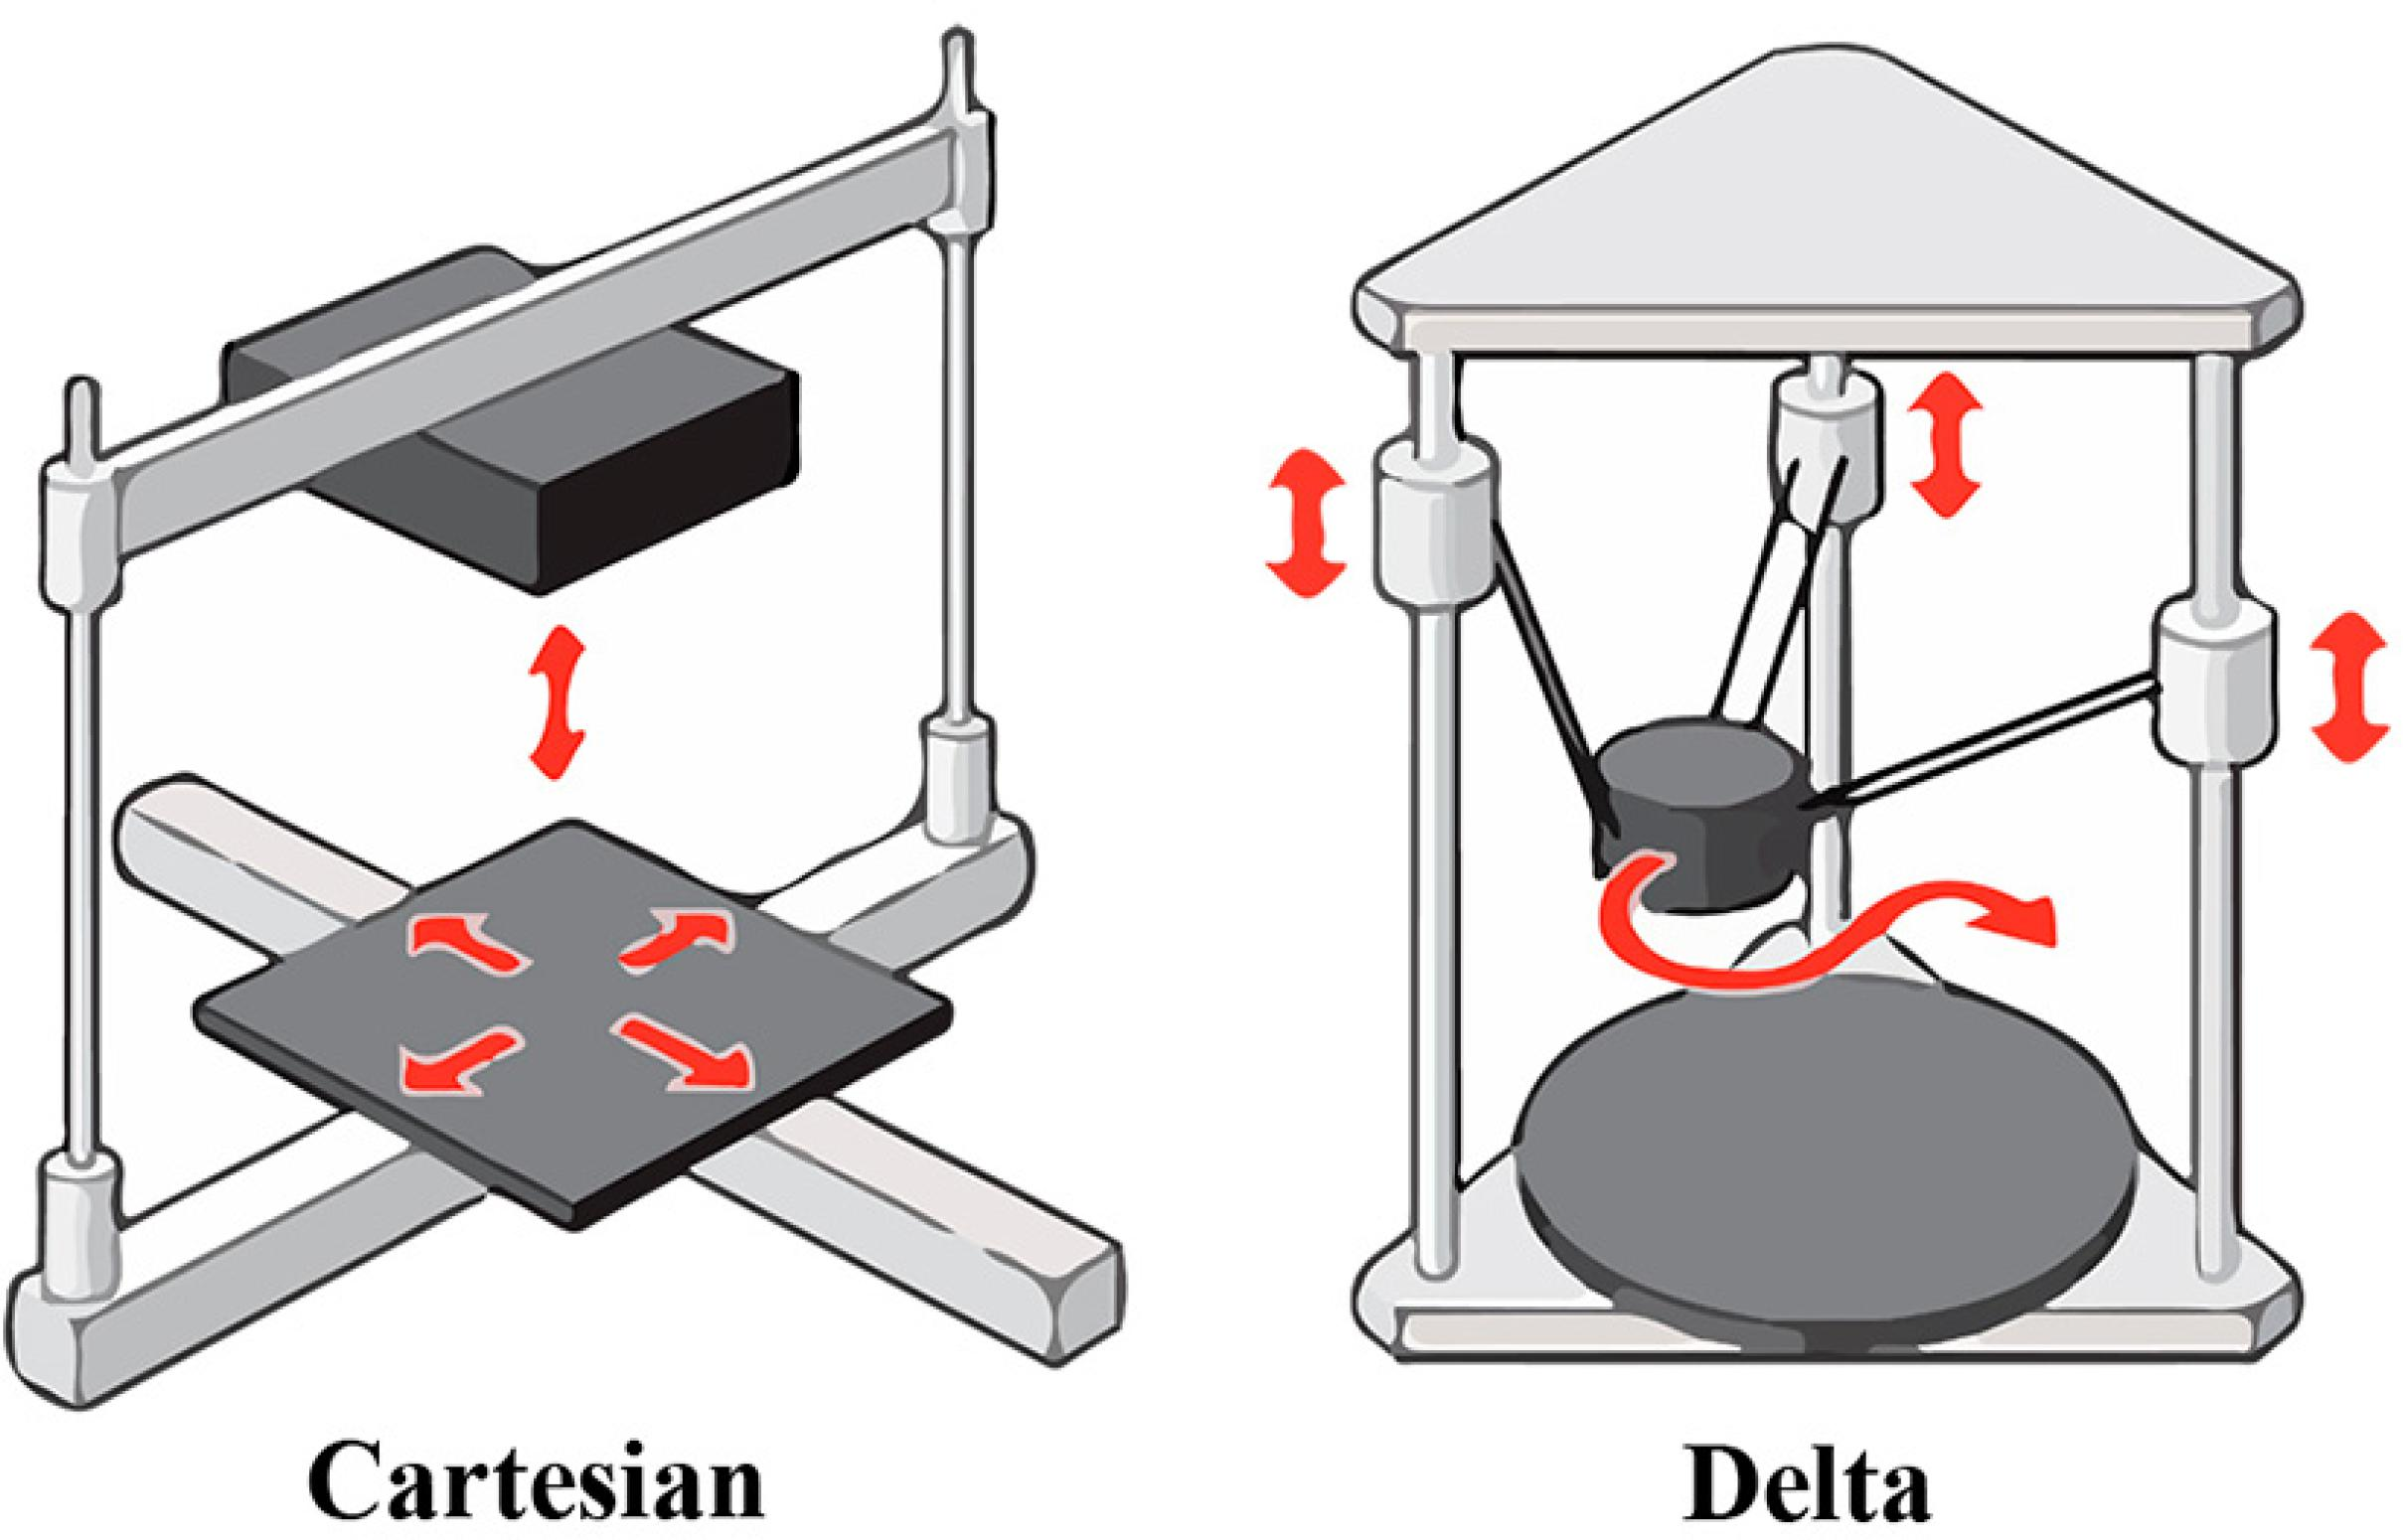
\includegraphics[width=0.40\textwidth]{chapter_2/figures/cartesiandelta.jpg}
    \caption{Comparison cartesian and delta system [scielo]}
    \label{fig:cartesiandelta}
\end{figure}

In this thesis, the focus will be on cartesian style printers, the specific system that will be used for investigation is the Ultimaker S5 system \cite{Ultimaker2019UltimakerSheet} shown in figure \ref{fig:Ultimaker}. The exturder is positioned through a machine code named g-code above the so called "printbed", "builplate" or "buildplatform" and deposits molten filament in a particular path along the x-y plane. After finishing the programmed path of a supposed "layer" the extruder moves up in the z direction to start depositing a new layer on top of the previous one. The part can be removed with little to no effort from the buildplate. The buildplate has often an implemented heating element to prevent large temperature gradients in the first layers, which can result in so called warping (due to difference in shrinkage in layers the corners of the part can start to curl, resulting in de-lamination from the buildplate), this is often an issue with materials with a high glass transition temperature and thermal expansion coefficients \cite{Turner2014AModeling}. 

\begin{figure}[H]
    \centering
    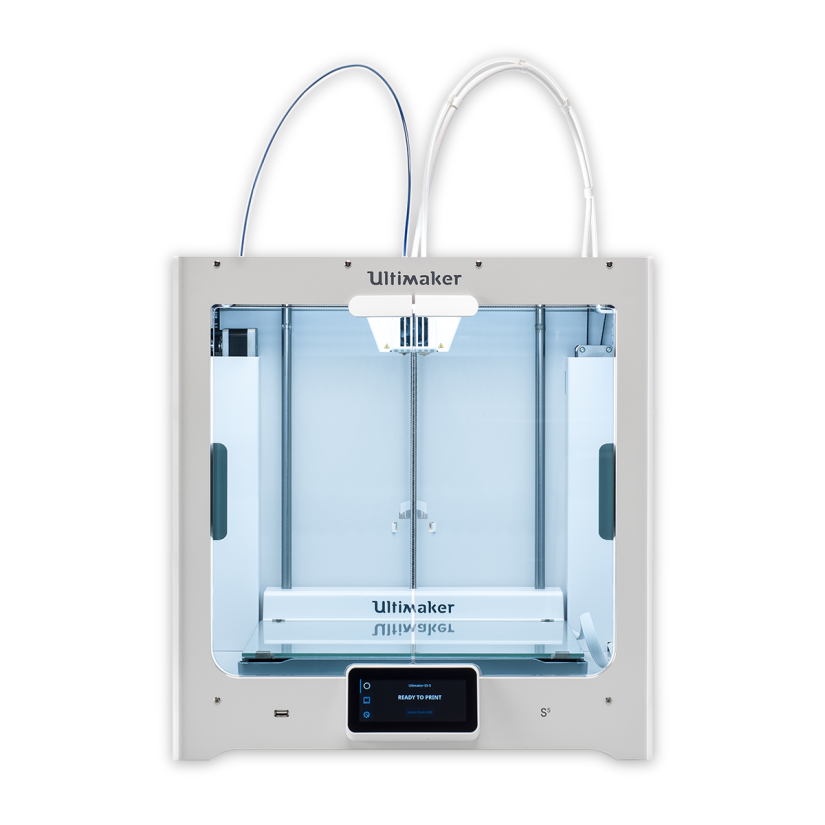
\includegraphics[width=0.40\textwidth]{chapter_2/figures/UltimakerS5.png}
    \caption{Ultimaker S5 \cite{Ultimaker2019UltimakerSheet}}
    \label{fig:Ultimaker}
\end{figure}

 Turner et al.\cite{Turner2014AModeling} have done a great job at clarifying the process and the effect it has on the product, the relevant concepts will be presented here. Note that this system is typical for consumer based FFF systems and is (generally) the basis for more advanced systems. It might happen that particular systems use different processes, for this thesis the process of the Ultimaker S5 is assumed. 

\begin{figure}[H]
    \centering
    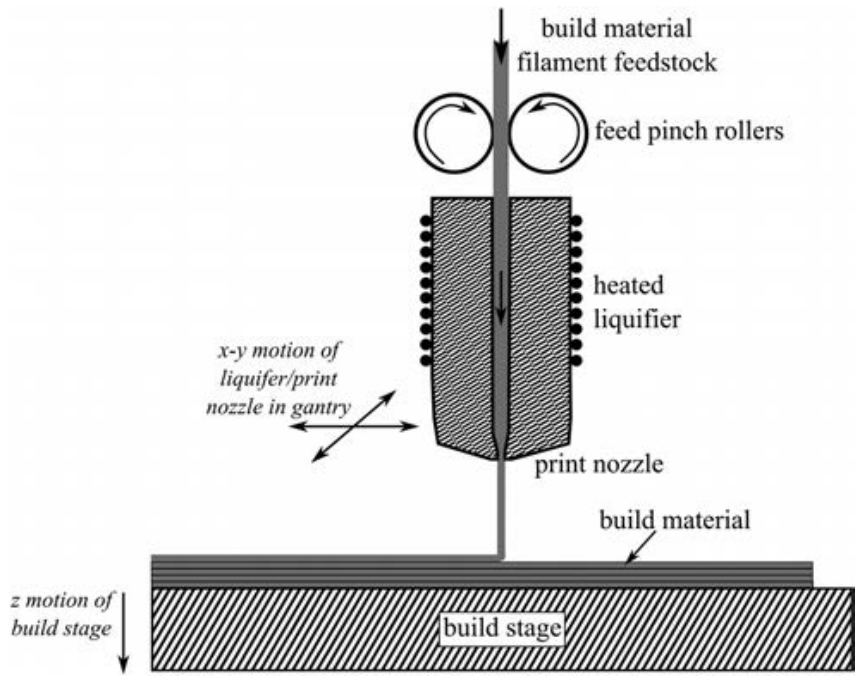
\includegraphics[width=0.50\textwidth]{chapter_2/figures/Wirefeedmechanism.PNG}
    \caption{Wire feed mechanism \cite{Turner2014AModeling}.}
    \label{fig:Wirefeed}
\end{figure}

\subsubsection{Feed mechanism}
    \label{Feed mechanism}
The feed mechanism is the root of the material supply, between two feed pitch rollers a filament of material is being pushed through a nozzle as can be seen in figure \ref{fig:Wirefeed}. The filament can be stored in a sealed container to prevent water absorption. Some materials are more prone to hygroscopy (like Nylon 66 and PLA), which during the extrusion results in the evaporation of the water and consequently in morphological changes in the material, blockages of the nozzle and formation of bubbles and porosity. This can be one of the issues of decreased mechanical properties, and should therefore be avoided. 

\subsubsection{Liquifier}
    \label{Liquifier}
The liquifier (figure \ref{fig:Wirefeed}) has a critical function: the softening of the polymer feed stock. This metal block has integrated heating elements to maintain a uniform temperature for liquefying the material.  A range of amorphous and semi-crystalline thermoplastic polymers (including fibers) with different melting and glass transition temperatures can be used in filament form as feedstock material. The liquifier temperature does normally not exceed 280$^{\circ}$C for consumer based systems, which excludes engineering polymers from use. It should be noted that due to the pressure and the shear force involved in the extrusion of filament through the nozzle, the polymer chains are being aligned in the direction of deposition (figure \ref{fig:polymerallignment}, which can have a significant impact on the mechanical properties of the part \cite{Mcilroy2017DisentanglementManufacturing}.

\begin{figure}[H]
    \centering
    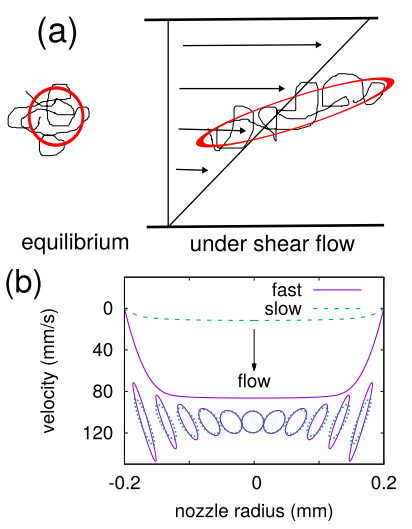
\includegraphics[width=0.4\textwidth]{chapter_2/figures/polymerallignment.PNG}
    \caption{a)Allignment of Polymer chains b)Velocity profile of polymer chains exiting the nozzle\cite{Mcilroy2017DisentanglementManufacturing}}
    \label{fig:polymerallignment}
\end{figure}

\subsubsection{Road deposition}
    \label{Road deposition}
The nozzle pushes hot filament onto the buildplate. During the extrusion the polymer melt is under stress, which reduces its volume due to deformation of energy being stored elastically. The nozzle hovers above the substrate at the prescribed layer height (often between 0.1 and 0.4mm), as can be seen in figure \ref{fig:Roaddepostion}. Consequently, the polymer melt is pushed outside and expands due to the absence of pressure. This phenomenon is called "dye swelling" and can be seen in figure \ref{fig:dieswelling}. Dye swelling plays a large role in the determination of the tolerance and surface roughness of a part. A ratio $(s)$ can be assigned to the swelling of the material with respect to the diameter of the die opening (nozzle). This value depends on the geometry of the nozzle, material properties (such as thermal expansion coefficient) and is generally in the range of 1.05 to 1.3. Shofner et al\cite{Turner2014AModeling} have found that the implementation of inelastic particles, such as short carbon fibers, have a positive effect of reducing the dye swelling, resulting in smoother surfaces (which is confirmed in empirical test with onyx, a carbon fibre filled nylon polymer \cite{TNO2017ProcesbegeleidingLearned}). 


\begin{figure}
\centering
\begin{minipage}{.5\textwidth}
  \centering
    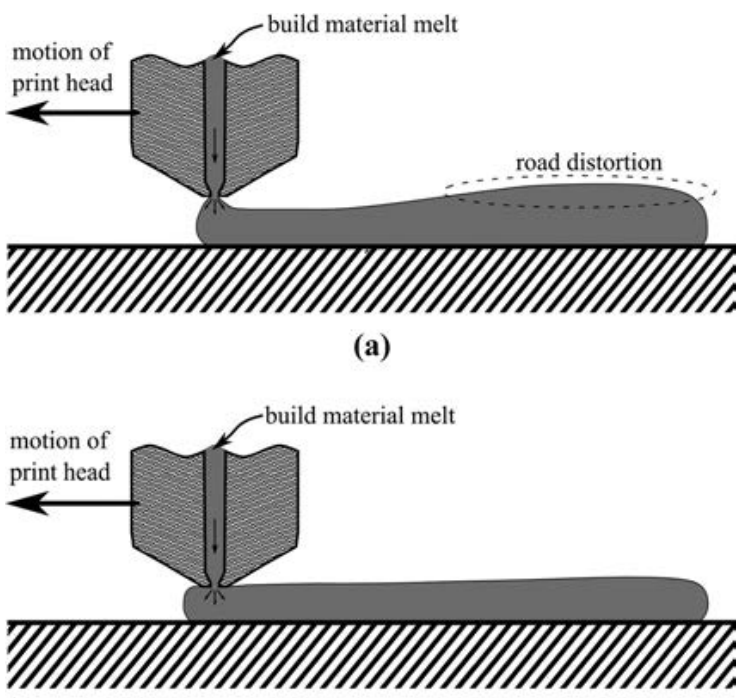
\includegraphics[width=.6\textwidth]{chapter_2/figures/Extrusion.PNG}
   \caption{Road deposition \cite{Turner2014AModeling}}
    \label{fig:Roaddepostion}
\end{minipage}%
\begin{minipage}{.5\textwidth}
  \centering
  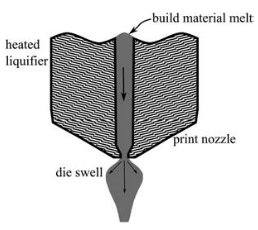
\includegraphics[width=.6\textwidth]{chapter_2/figures/dieswelling.PNG}
    \caption{Die swelling \cite{Turner2014AModeling}}
    \label{fig:dieswelling}
\end{minipage}
\end{figure}

The so called "bead" or "road" is deposited in an oblong shape (similar to a stadium shaped oval), and starts to cool due to convective cooling once it comes in contact with air and conductive cooling once it comes in contact with neighbouring roads. Bellini et al. \cite{Bellini2003MechanicalModeling} modeled this convective cooling assuming a heat transfer coefficient of $h =20 W/m^2$. In chapter 4 further investigation will be conducted on the shape of the road. Interestingly enough, the thermal conductivity of the feedstock material has a positive effect on the temperature of the bead after deposition. Instead of losing heat due to high thermal conduction, materials with high conductivity can more easily extract heat from the hot end at a larger distance, therefore creating better bonding between layers. 

\begin{figure}[H]
    \centering
    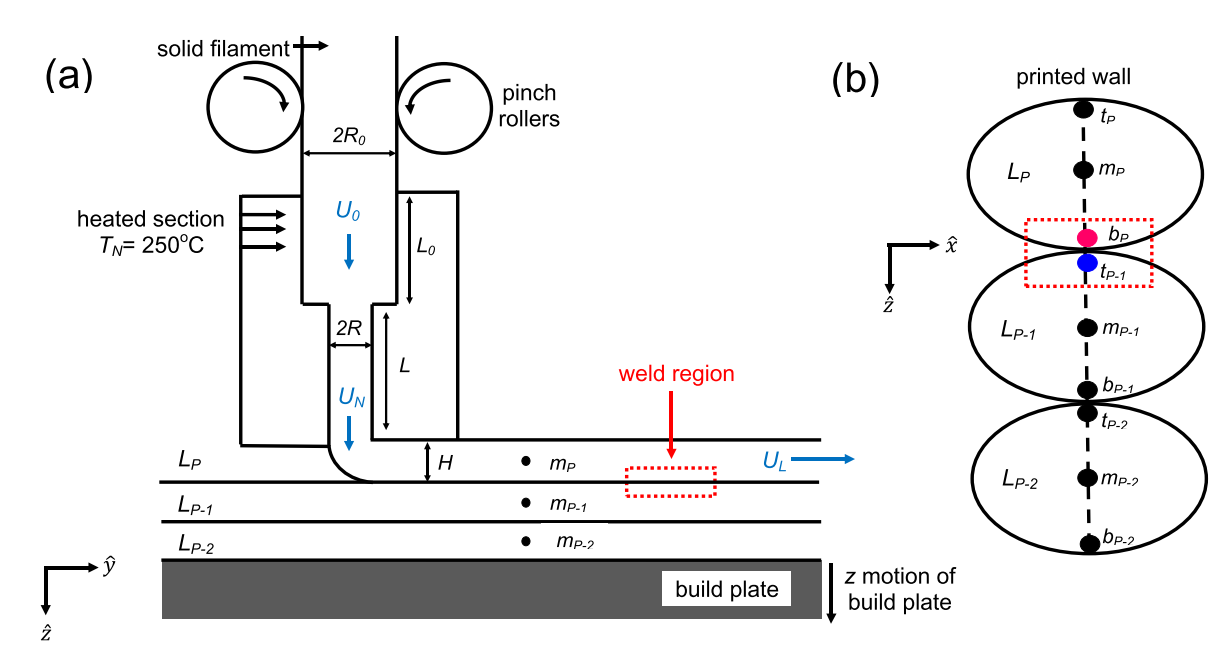
\includegraphics[width=0.7\textwidth]{chapter_2/figures/welding.png}
    \caption{a)Welding of subsequent roads. b)Heated top layer contacts with cooled lower layer \cite{McIlroy2017DeformationManufacturing}
    \label{fig:welding}}
\end{figure}

The touching surfaces of the roads are "welded" together if the temperature of both roads is high enough (figure \ref{fig:welding}). The deposited filament is practically uniformly melted, since the liquifier temperature is set at a higher temperature than the melting temperature ($T_m$) or glass transisition temperature for thermoplastics ($T_g$). For perfect bonding the surface of the lower road should also reach this temperature and maintain this for enough time. However, the temperature of the lower road has cooled since it was deposited. The strength of the bond is therefore a function of time and temperature of both roads and can be expressed in two different mechanisms: wetting and healing (figure \ref{fig:polymerwelding}). This is an anisothermal process of heating and cooling different layers at high rates as can be seen in figure \ref{fig:temperaturehistory}. One of the first researchers that began investigating this process where Thomas and Rodriguez \cite{Thomas2000ModelingRoads} followed by Bellehumeur et al.\cite{Bellehumeur2004ModelingProcess}and  Sun et al. \cite{Sun2008}. Seppala et al. \cite{Seppala2017WeldManufacturing} did an extensive study on the temperature profile of extruded roads and the bond forming after different layers are being deposited on top of it. The temperature history can either empirically be observed with an infrared camera, or can numerically be approximated when the toolpath of the extruder is known.There are currently software tools available which will generate a predicted temperature profile for specific layers in a particular FFF produced geometry\cite{Digimat-AM}. 

\begin{figure}[H]
    \centering
    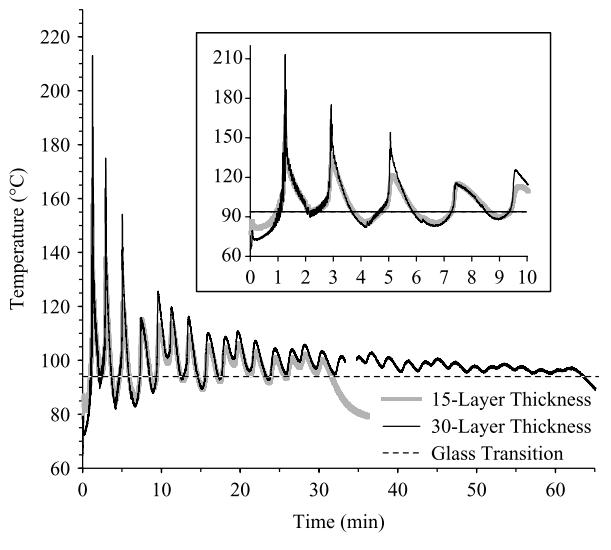
\includegraphics[width=0.4\textwidth]{chapter_2/figures/temperaturehistory.PNG}
    \caption{Temperature profile of the bottom filament \cite{Sun2008}
    \label{fig:temperaturehistory}}
\end{figure}

Wetting is defined by Wool \cite{WoolStrenghtInterfaces} as close molecular contact (van der Waals bonds) when two pieces of molten polymers are brought into contact followed by inter diffusion of chain segments back and forth across the wetted interface. The diffusion of polymer chains is called healing, which is investigated by Sun et al \cite{Sun2008}. After wetting of the roads, neck growth occurs which widens the area between adjunct roads. These three processes can be seen in figure \ref{fig:polymerwelding}. 

\begin{figure}[H]
    \centering
    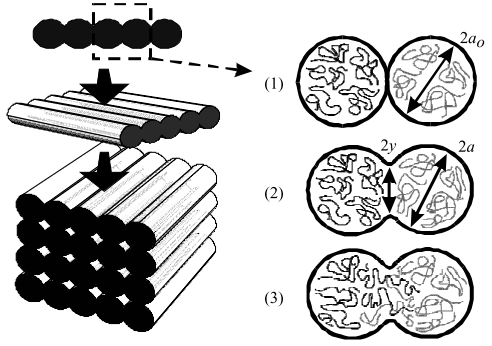
\includegraphics[width=0.4\textwidth]{chapter_2/figures/polymerwelding.PNG}
    \caption{Bond formation between roads: (1) contact, (2) wetting and necking (3) healing  \cite{Sun2008}}
    \label{fig:polymerwelding}
\end{figure}

After subsequent roads are deposited in layers on top of each other, a particular "mesostructure" of welded beads, with an elliptical shape, will appear. These mesostructures (shown in figure \ref{fig:mesostructure}) are analyzed in different articles \cite{Somireddy2017MechanicalMesostructure}
\cite{Somireddy2018DevelopmentFDM}
\cite{Li2002CompositeProperties} \cite{Rodriguez2001MechanicalInvestigation}
\cite{Rodriguez2003MechanicalModeling}
\cite{Blok2018AnComposites} 
\cite{Sun2008}, all conclude that the mesostructre has significant impact on the mechanical properties.
Most of the researchers used microtoming and optical microscopy to produce clear images (in the range of tenths of millimeters) of the mesostructure. These voids form a significant amount of porosity which has an adverse effect on the mechanical properties, resulting in stress concentrations and leading to premature brittle failure  near the porous region.  What is not observable in the mesostructure is the degree of healing between the roads. 
The majority of above mentioned the researchers do not provide satisfactory information regarding their process settings or hardware used. Early experiments often incorporated Stratasys systems with their own produced ABS P400, due to their early market share. 

The final shape of the road depends on the surface tension, feed rate, viscosity, rate of cooling and interaction with the print head. There have been attempts of modelling the shape and spreading of the roads without being successful. A model proposed in the work of Turner \cite{Turner2014AModeling} assumes full wetting but does not account for the change of viscosity. The result significantly differs from empirical observations. 

\begin{figure}[H]
    \centering
    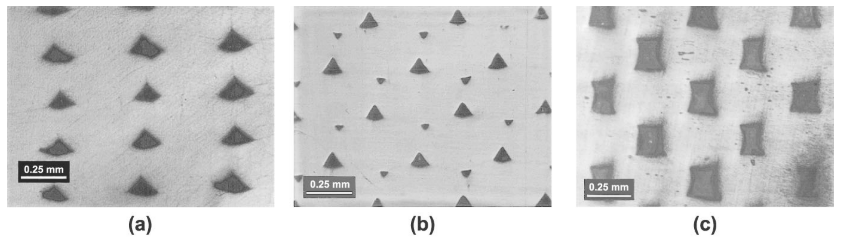
\includegraphics[width=1\textwidth]{chapter_2/figures/Mesostructure.PNG}
    \caption{Different types of mesostructures \cite{Rodriguez2001MechanicalInvestigation}}
    \label{fig:mesostructure}
\end{figure}

According to Sun, the amount of wetting and healing determines largely  the mechanical properties of the part \cite{Sun2008}. The healing of the polymer are related to the polymer material property called reptation time, which is the time a polymer needs, at a certain temperature, to "reptate" out of the other chains of the melt to acquire a new random position. Reptation is closely related to the glass transition temperature ($T_g$), the temperature where polymers start to diffuse and lose viscosity. After reaching this temperature polymer chains start to reptate exponentially faster. Different authors \cite{Mcilroy2017DisentanglementManufacturing}  \cite{Hart2018IncreasedAnnealing} \cite{Bartolai2016PredictingManufacturing} assume perfect bonding (full reptation) to be comparable to the mechanical properties of the middle of the road. With the help of WLF (Williams-Landel-Ferry graphs) a model can be made where reptation time is plotted as a function of temperature (figure \ref{fig:WLFreptation}). By producing a set of empirical data-points the WLF curve can be extrapolated \cite{Peterson2019ReviewPerspective}. With a higher temperature the amount of time needed for perfect healing is reduced, this can e.g. be achieved with a heated chamber or "envelope". According to Bartolai et al. \cite{Bartolai2016PredictingManufacturing} the strength of a road weld can be predicted using the following equation:

\begin{equation} \label{eq:weld}
\frac{\sigma_{weld}}{\sigma_{UTS}}=\left(\frac{t_{weld}}{t_{rep}}\right)^{1/4}
\end{equation}

In this equation $\sigma_{weld}$ is the weld strength in (MPa), $\sigma_{UTS}$ is the bulk ultimate tensile strength (in MPa), $t_{weld}$ is the time of molecular activity at a defined temperature (accodring to the WLF graph) at the interface (in seconds), and $t_{rep}$ is the time average reptation time of the polymer (in seconds). As $t_{weld}$ approaches $t_{rep}$ the polymer becomes fully healed and best strength is achieved. In the (limited) validation and verification of Bartolai, the conclusion was the of $\sigma_{weld}$ weld can be quite difficult for an accurate prediction.

\begin{figure}[H]
    \centering
    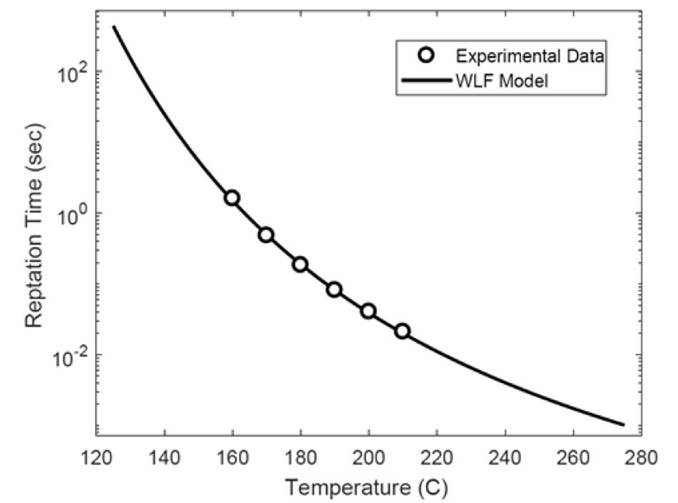
\includegraphics[width=0.4\textwidth]{chapter_2/figures/WLFreptation.PNG}
    \caption{WLF model, reptation time is a function of temperature \cite{Seppala2017WeldManufacturing}}
    \label{fig:WLFreptation}
\end{figure}

\subsubsection{Build plate and chamber}
    \label{Build plate and chamber}
The liquefied filament is deposited on the build plate (also called printbed) and is consequently deposited on top of the previous layers. The buildplate can be as simple as a piece of metal or glass. However, there are some crucial aspects concerning the properties of the bed. The adhesion of the first deposited layer with the bed is very important to prevent de-lamination during the process. Therefore, heat elements are used to decrease steep heat gradients in the part, which result in warping. To prevent the bed itself from deforming (as little as a few hundredth of a mm can have negative impact on the first layer) a material with a low thermal expansion coefficient is chosen (e.g. glass). The bed temperature has a positive effect on the layer bonding in the lower region of the part. However, this is only "felt" in roughly the first centimeters of the part trough conduction. It has been concluded that a higher overall temperature of the chamber has a beneficial impact on the road healing and subsequently on the mechanical properties\cite{VeenEnhancingTemperature}. More advanced systems therefore implement a heated envelope.

\subsection{Process parameters}
    \label{Process parameters}
Since the process parameters of the FFF process have major influence on the resulting parts, it is essential to analyze the parameters and identify their influence on the mechanical properties. In this section the important parameters are highlighted.

%part about slicers
Most of these setting are defined by the so called "slicer" software, which is used to edit setting before generating a machine code that can be read by the printer. Certain machines have unique compatibility with a certain slicer (e.g. Eiger software from Markforged), or are produced by a manufacturer which also allows compatibility with other FFF systems (e.g. Cura from Ultimaker) or are produced  by a third party software developer (e.g. Simplify 3D, Slic3r). These softwares have similar settings that can be adjusted which will result in a  trade-off between speed and weight versus resolution, precision and mechanical performance. Since this thesis is mostly based on an Ultimaker S5 system \cite{UltimakerUltimakerS5}, and Cura is used as its slicer by the manufacturers, the terminology and parameters of Cura will be used as a benchmark. 

The most significant parameters that have effect on the product are:
- Layer height (mm)\\
- line width (mm)\\
- Feed rate (mm$^3$/s)\\
- Extrusion temperature ($^{\circ}$C)\\
- Envelope temperature ($^{\circ}$C)\\
- Build plate temperature ($^{\circ}$C)\\
- Travel speed (mm/s)\\
- Infill density (\%)\\
- Infill orientation and shape ([a b c])\\
- (negative) Airgap (mm)\\


Regular slicers use different type of settings for  different elements in a part. Let's consider the cross section of a cube (as can be seen in figure \ref{fig:Shell}) for FFF printing. Once a CAD (computer aided design) file (often in the form of a STL "stereolithography" file) or other geometrical digital drawing supported by the slicer is uploaded, the slicer will define different settings for different elements. Most important being: Bottom layers, Outer shell (walls), top layers, infill. The effects of the  elements will be outside the scope of this thesis and can be easily found online (3Dhubs \cite{3Dhubs3DHubs}, All3D \cite{all3dpAll3dp}, Ultimaker \cite{UltimakerUltimakerSheet}, Simplify 3D\cite{Simplefy3DPrintGuide}). For this project the focus is on a part with only bottom-layers, mimicking fully "dense" parts. Applying only bottom layers will generate parts with best mechanical properties per volume.   \cite{Li2017TheProperties}

\begin{figure}[H]
    \centering
    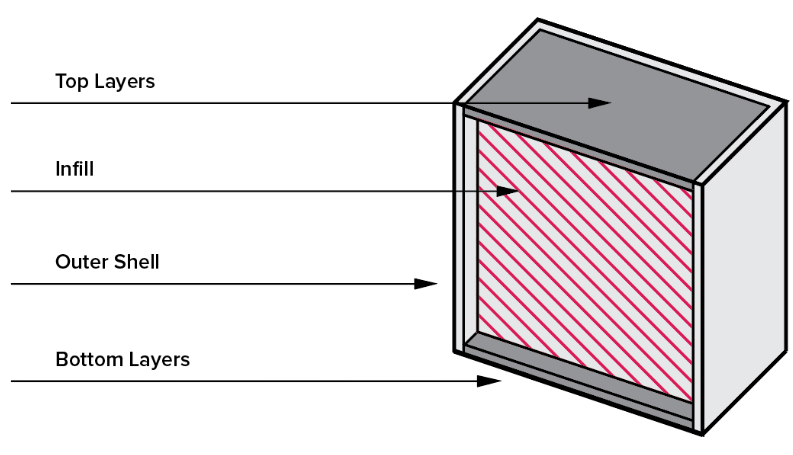
\includegraphics[width=0.5\textwidth]{chapter_2/figures/Shell.PNG}
    \caption{Elements of a 3D printed part \cite{3DHubsIntroductionPrinting}}
    \label{fig:Shell}
\end{figure}
Effort that needs to be highlighted is the work of  Li et al. \cite{Li2017TheProperties} who generated empirical data and derived numerical models displaying the relation of temperature related parameters with the tensile strength of PLA, while maintaining other parameters constant.

According to parameters studied by Ahn et al. \cite{Ahn2002AnisotropicABS} the air gap and raster orientation are the parameters most significantly affecting the mechanical properties. This is explained by the fact that the air gap is directly linked with the porosity and the raster orientation is directly linked with the stress applied at the road interfaces.
A similar but more extensive research has been conducted by Mohamed et al. \cite{Mohamed2016EffectExperiment}, resulting in the same conclusion.

\subsubsection{Layer height}
The layer height is the height of one layer, subsequently also the height of one road. Increasing this parameter will decrease the print time proportionally, the drawback is higher surface roughness, larger porosity, larger stress concentration points and worse layer bonding. In Cura the layer height is limited between 0.04 and 0.32 mm. Since the polymer is welded by applying pressure and heat, different researchers assume that the roads have a horizontal and vertical overlap. This is about 10\% according to Somireddy \cite{Somireddy2017MechanicalMesostructure}.  The emperical results of Li et al. \cite{Li2017TheProperties} regarding the layer height parameter are shown in figure \ref{fig:Layerheigth}.

\begin{figure}[H]
    \centering
    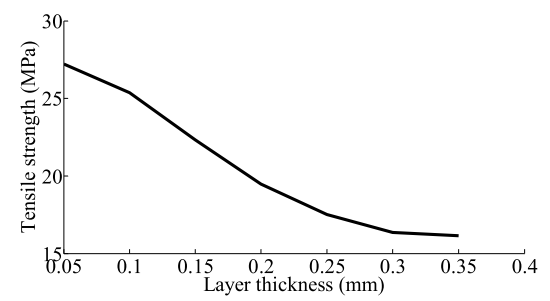
\includegraphics[width=0.5\textwidth]{chapter_2/figures/Layerheight.PNG}
    \caption{Layer height against tensile strength for XY[45/-45] samples \cite{Li2017TheProperties}}
    \label{fig:Layerheigth}
\end{figure}

Li \cite{Li2017TheProperties} explains that a smaller layer height will actually increase bonding between roads. High conductivity combined with the small volume that needs to be heated will positively affect the temperature history of the interface, compared to thicker layer heights where the heat flux is not able to heat the material as much as for the thinner counterparts. This is also confirmed by Kuznetsov \cite{Kuznetsov2018StrengthProcess}, who additionally claims that a reduced layer height also limits porosity in a part.

\subsubsection{Line width}
This process parameter can be misleading. According to Somireddy \cite{Somireddy2017MechanicalMesostructure} FFF systems produce roads that are set to have a 10\% overlap with its neighbouring roads in the xy plane. The line width defines the distance between adjacent roads, which could be assumed as nominal line width or the distance between roads. According to him the extruded line width is therefor about 10\% wider, if one would extrude a single road with a line width of 0.4 mm and a layer height of 0.2 mm it would be observed that a 10\% larger ellipse is produced. 
%By personal observation it was observed that multiple single roads deposited on top of each other produce a width that is 5-10\% larger than the nominal line width. 
This is in line with the observed increase in dimension for the production of fitted parts. A similar theory is proposed by Hodgson \cite{GaryHodgsonSlic3rMath}, "Extrusion Width is the thickness of a single filament extruded either in free air or above a surface. It's not the distance of two adjacent paths since some overlap will be generally applied in order to get better bonding."
When printing only bottom layers the roads are constrained by the substrate on the bottom, by the nozzle on the top, and possibly by a road on one side.  In figure \ref{fig:roadconnecting} the sintering of roads can be observed. The problem with this model is the fact that the overlapped material is not accounted for. In the chapter 4 a new model will be presented. There is currently not a consensus on the form of the mesostructure, this is partly due to large development and  variety of printers and available printer settings.

\begin{figure}[H]
    \centering
    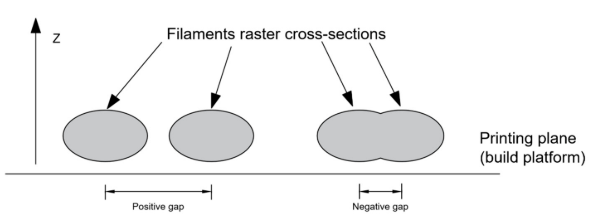
\includegraphics[width=0.7\textwidth]{chapter_2/figures/roadconnecting.PNG}
    \caption{A schematic representation of filament cross-sectional areas, showing the difference between positive and negative gaps \cite{Cuan-Urquizo2019CharacterizationApproaches}}
    \label{fig:roadconnecting}
\end{figure}

The range of the line width process parameter is limited by the nozzle diameter. For a nozzle of 0.4mm Cura allows for a line width ranging between 0.25 to 0.8. According to Montero \cite{Montero2001MaterialExperiments} a variation in line width has no significant effect on the mechanical properties of the part. Thomas \cite{Thomas2000ModelingRoads} and  Kuznetsov\cite{Kuznetsov2018StrengthProcess} notice a positive effect in inter-road bonding with increased line width.
%due to the larger  volume which cause prolongation of high temperature in the contact points and a reduction in porosity.  
%[for revision] The slicer always calculates the roads to be tangent, meaning that a 4mm wide beam will generate 10 0.4mm wide roads. Increasing this will have similar effects as increasing the layer height. This generates often just enough polymer to sinter the surfaces together, in comparison with the layer height, the different roads are not aided by gravity for better bonding. Be aware that the line width can also be influenced by inconsistencies of the filament. Filaments for the ultimaker have a nominal diameter of 2.85 +- 0.05, which mean that the road line width might have a fluctuation of 2\%.

\subsubsection{Airgap}
The airgap is defined as the gap in between different roads in the xy plane (intra-laminar) figure \ref{fig:roadconnecting}. Generating an airgap that is the same size of your road width will half your infill density, creating an negative airgap will produce an overlap between roads. It is not possible to select a negative value in Cura (implying an overlap of roads). This was possible in the Stratasys slicer settings, and has been thoroughly studied in different experiments \cite{Somireddy2017MechanicalMesostructure}  \cite{Rodriguez2001MechanicalInvestigation}   \cite{Ahn2002AnisotropicABS}  \cite{Dawoud2016MechanicalTechniques} \cite{Gebisa2018InvestigatingExperiment}
\cite{HossainImprovingParameters}
and resulted in higher density and mechanical properties (increase of about 5-10\% in $E_{11}$, $E_{22}$ and a 10\% increase in $G_{12}$) at the cost of speed and higher surface roughness and distortion. Additionally, the excess material can be accumulated on the nozzle and the part itself. Gebisa et al. \cite{Gebisa2018InvestigatingExperiment} claim that a negative airgap has also a negative influence on the heat transfer since the roads are deposited very close to each other and that more room facilitates the spread of semi-molten material between the gaps, resulting in structurally stronger parts. The conclusion of most experiments is that for ABS a negative airgap of not more than 10\% can lead to improvements in mechanical properties without significant influence on the dimensional accuracy and surface quality. It appears that  slicers have optimized this phenomena in the past years to achieve minimal porosity \cite{GaryHodgsonSlic3rMath}. Simplify 3D has the option to enhance the infill extrustion width for only the infill (Cura can only modify it for the whole part).
If we consider Somireddy's \cite{Somireddy2017MechanicalMesostructure} mesostructure images for regular settings a 10\% overlap is observed,  if the line width is reduced with 10\% while the extruded width remains equal,  approximately 20\%overlap is observed figure \ref{fig:Meso10&20}. The section \ref{mesostructure} will address this subject in more detail.
We can conclude from this analysis that negative airgap has an optimum where the mechanical properties are optimized without significantly distorting the surface of the product, it seems that this is already applied in some slicers. 

\begin{figure}[H]
    \centering
    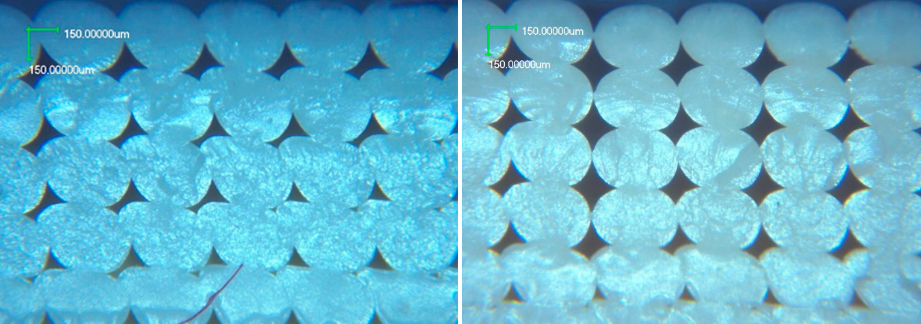
\includegraphics[width=0.5\textwidth]{chapter_2/figures/Meso10and20.jpg}
    \caption{20\% overlap (left) 10\% overlap (right)\cite{Somireddy2017MechanicalMesostructure}}
    \label{fig:Meso10&20}
\end{figure}

\subsubsection{Feed rate}
The feed rate is the volume of filament that is extruded per timescale. Since this is automatically calculated by Cura as a function of the layer height, line width and speed, it is difficult to precisely enhance, therefore it is defined as a multiplier of the default setting. Adjusting this will multiply the original calculated feed rate with a defined factor. This can for example fix under-extrusion (figure \ref{fig:underextrusion} when the feed rate is too low, resulting in bad bonding and large gaps) which is detrimental for the mechanical properties of the part. It can also compensate for over-extrusion \ref{fig:overextrusion}, which is detrimental for tolerance and accuracy. However, this could also be used to increase the extrusion to generate the so called "negative air gap". By increasing the flow multiplier, a wider road can be deposited without an increase in distance between roads as would happen with increase line width. This could be a detour to achieve the same increase in mechanical properties as a negative air gap would have.
We can conclude that the feed rate is closely related to the negative airgap parameter. The theory presented above and at the subsection of "line width" is supported by Patanwala et al. \cite{Patanwala2018TheComposites}, who wrote an detailed report on the characterization of the flow rate and bonding of carbon nanotubes-PLA composites.  
\begin{figure}
\centering
\begin{minipage}{.5\textwidth}
  \centering
    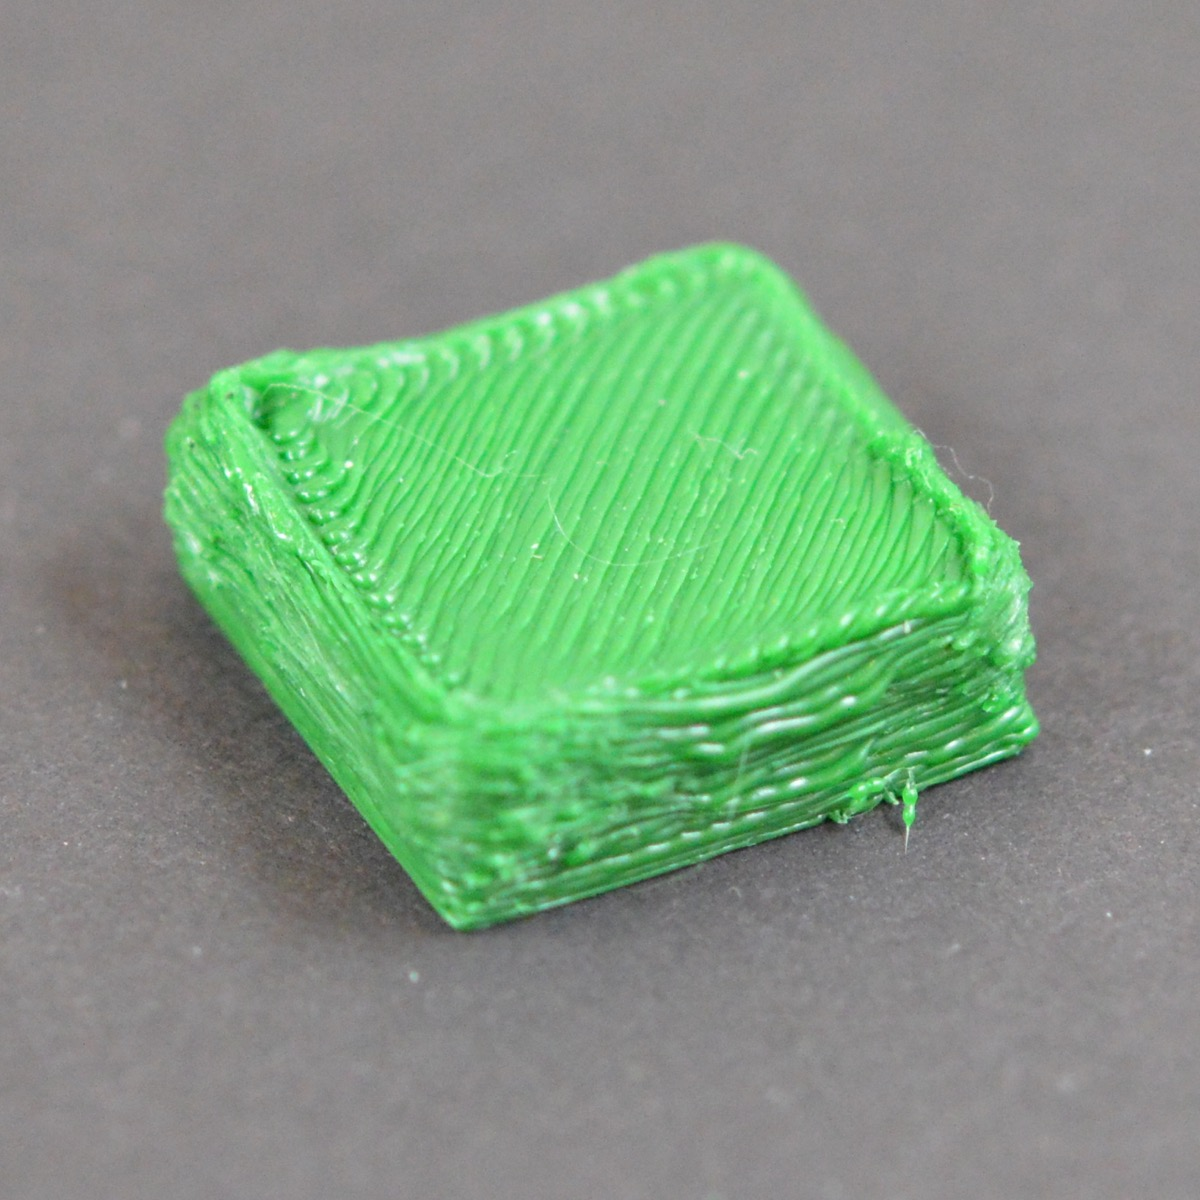
\includegraphics[width=0.6\textwidth]{chapter_2/figures/overextrusion.jpg}
    \caption{Overextrusion generating distortion of the part \cite{Simplefy3DPrintGuide}}
    \label{fig:overextrusion}
\end{minipage}%
\begin{minipage}{.5\textwidth}
  \centering
    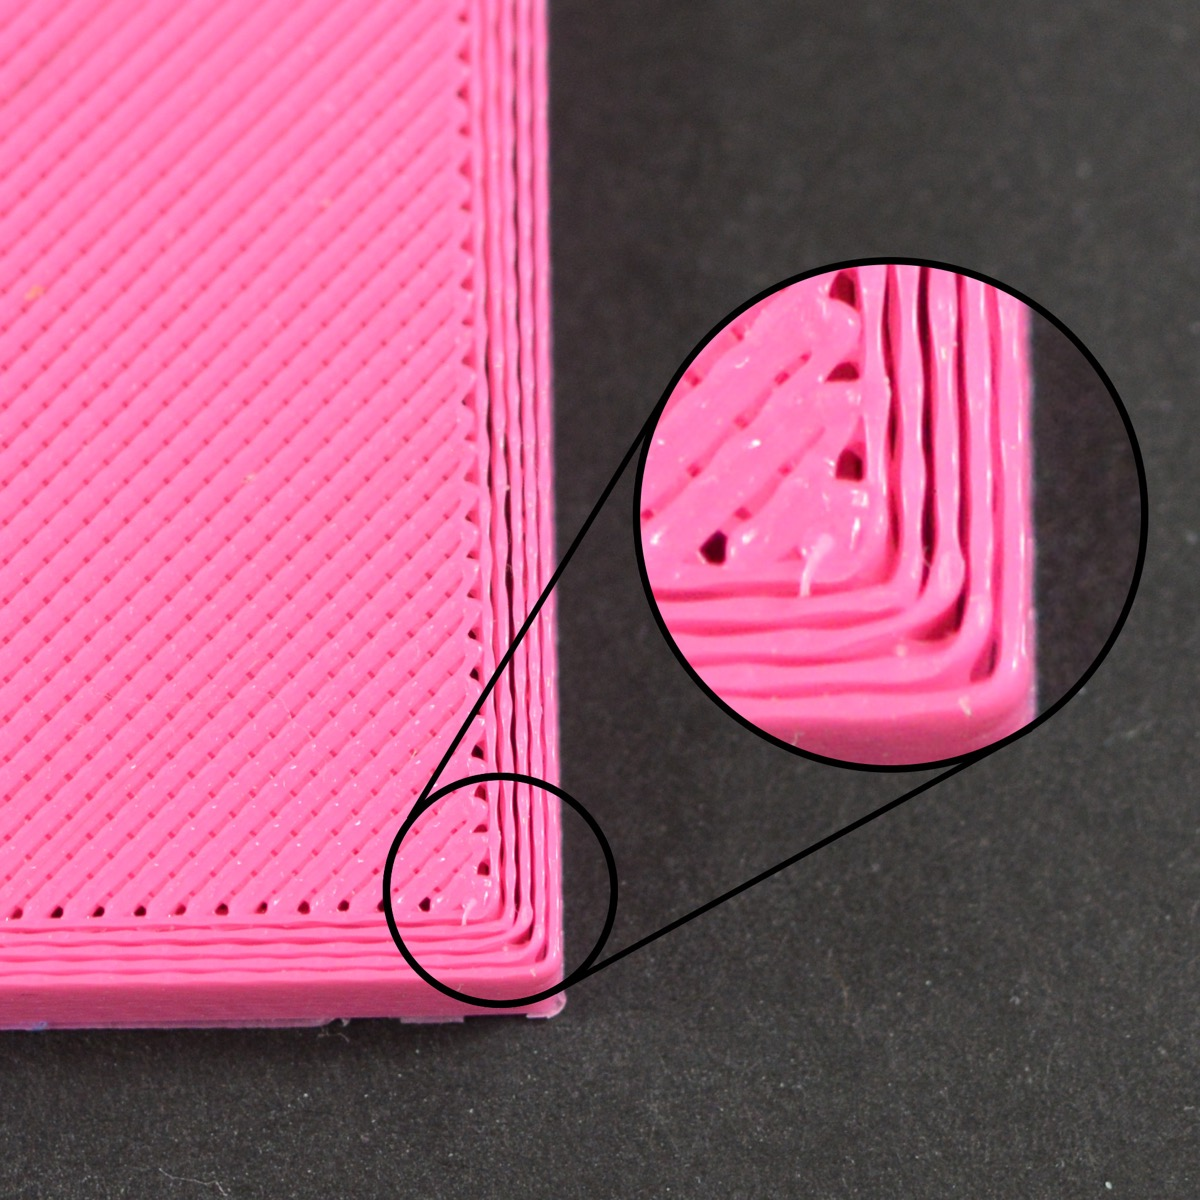
\includegraphics[width=0.6\textwidth]{chapter_2/figures/underextrusion.jpg}
    \caption{Underextrusion generating limited contact areas between roads \cite{Simplefy3DPrintGuide}}
    \label{fig:underextrusion}
\end{minipage}
\end{figure}

\subsubsection {Extrusion temperature }
The extrusion temperature is defined as the constant temperature of the extruder. This setting is different for every material. To make a material flow more the temperature can be increased, this can help for very fast prints, or in the case of underextrusion. The dangers of printing too hot are, especially for small sections, a distortion of geometry due to a drop in viscosity. If the temperature is too low, the filament is too viscous to be extruded out of the nozzle, resulting in under extrusion or extrusion issues.  
There is an optimal range for the extrusion temperature which has been studied by Montero \cite{Montero2001MaterialExperiments} and others.
%as can be seen in figure \ref{fig:Montero}

\subsubsection {Envelope temperature }
Advanced FFF systems include a heated chamber or envelope. This is applied to increase the bonding of the roads, different studies \cite{Sun2008} \cite{Bellehumeur2004ModelingProcess} have shown that the bonding properties (healing and wetting) are affected by temperature and time. The downside is the possibility of small segments being heated too much, which results in distortion. The optimal envelope temperature for semi-crystalline materials is between $T_g$ and $T_m$. For amorphous polymers this is more problematic, since they do not have a specific melting temperature, instead they have a plateau after $T_g$ as can be seen in figure \ref{fig:EvsT}, the first observation would be to not exceed the temperature of this plateau.
According to van Veen \cite{Veen2019EnhancingTemperature} a clear relation was found between the envelope temperature and the bonding between layers, this is supported by the healing theory. 

\begin{figure}[H]
    \centering
    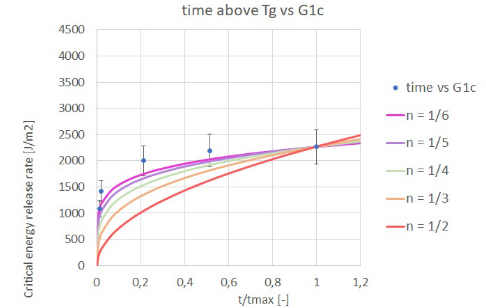
\includegraphics[width=0.5\textwidth]{chapter_2/figures/Dennisgraph.png}
    \caption{Critical release energy rate vs. the time parts spend above Tg\cite{VeenEnhancingTemperature}}
    \label{fig:Dennisgraph}
\end{figure}

\subsubsection {Build plate temperature }
 The buildplate temperature is generally near the $T_g$ to limit thermal stresses and warping. As a beneficial side effect, it constantly heats up a set of layers touching the buildplate.
The quantitative effects of the build plate temperature on the mechanical properties of the part have not been studied yet. 
%possible conduction laws, predicting temperature??

\subsubsection {Print speed }
Print speed proportionally alters the process times,  but comes at a cost of larger in-homogeneity. Due to a large amount of accelerations the feed rate can differ trough-out the part. Often over-extrusion is observed near the walls of a layer.

A low speed (approximately 35 mm/s) should be used to avoid large speed differences \cite{Li2017TheProperties}.  In figure \ref{fig:speedgraph} the dependency of the speed related to the position is shown.

\begin{figure}[H]
    \centering
    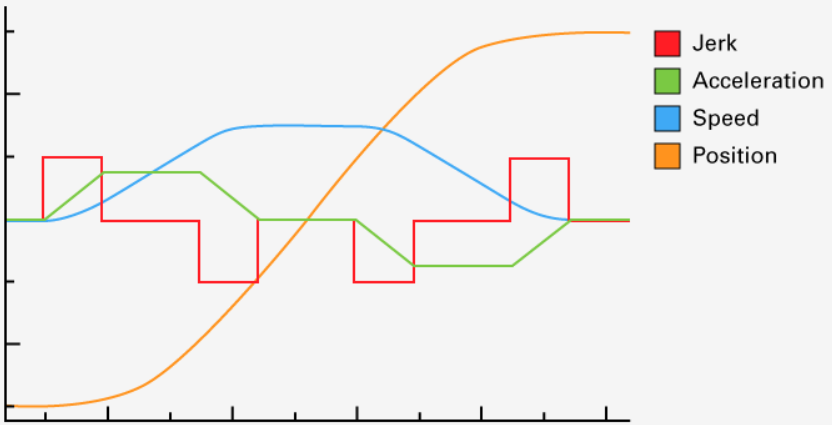
\includegraphics[width=0.4\textwidth]{chapter_2/figures/Speedgraph.PNG}
    \caption{Speed graph of the toolhead while printing \cite{UltimakerSpeed}}
    \label{fig:speedgraph}
\end{figure}

Li \cite{Li2017TheProperties} also investigated the effect of the deposition velocity on the tensile strength as can be seen in figure \ref{fig:depositionspeed}

\begin{figure}[H]
    \centering
    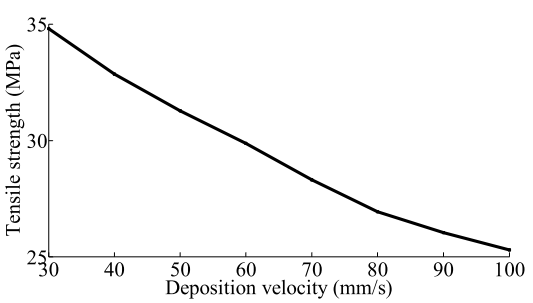
\includegraphics[width=0.3\textwidth]{chapter_2/figures/depostionspeed.PNG}
    \caption{Deposition velocity against tensile strength for XY[45/-45] samples \cite{Li2017TheProperties}}
    \label{fig:depositionspeed}
\end{figure}

Print speed directly influences the feed rate, which is most likely the cause of a decrease in mechanical properties with an increasing speed. Li also explains that for slower speeds the bottom layers remain at a temperature higher than $T_g$ for a longer period of time, which suggest that the adjacent filaments have more time to bond.

\subsubsection{Infill density}
The infill percentage determines the percentage of material with respect to air used in the infill structure. The infill is generally enclosed by so called wall layers (also called perimeters) and top and bottom layers. These roads form a solid shell on the surface. This volume of the infill can have different geometries, ranging from simple rectangles, to intricate 3D patterns as can be seen in figure \ref{fig:Infill}. The density can be changed in a variety of forms, creating thicker lines, more lines, direction etc. For this thesis the focus will be on structurally optimized parts, which includes 100\% infill (which won't result in a related relative density since there is a high amount of porosity).

\begin{figure}[H]
    \centering
    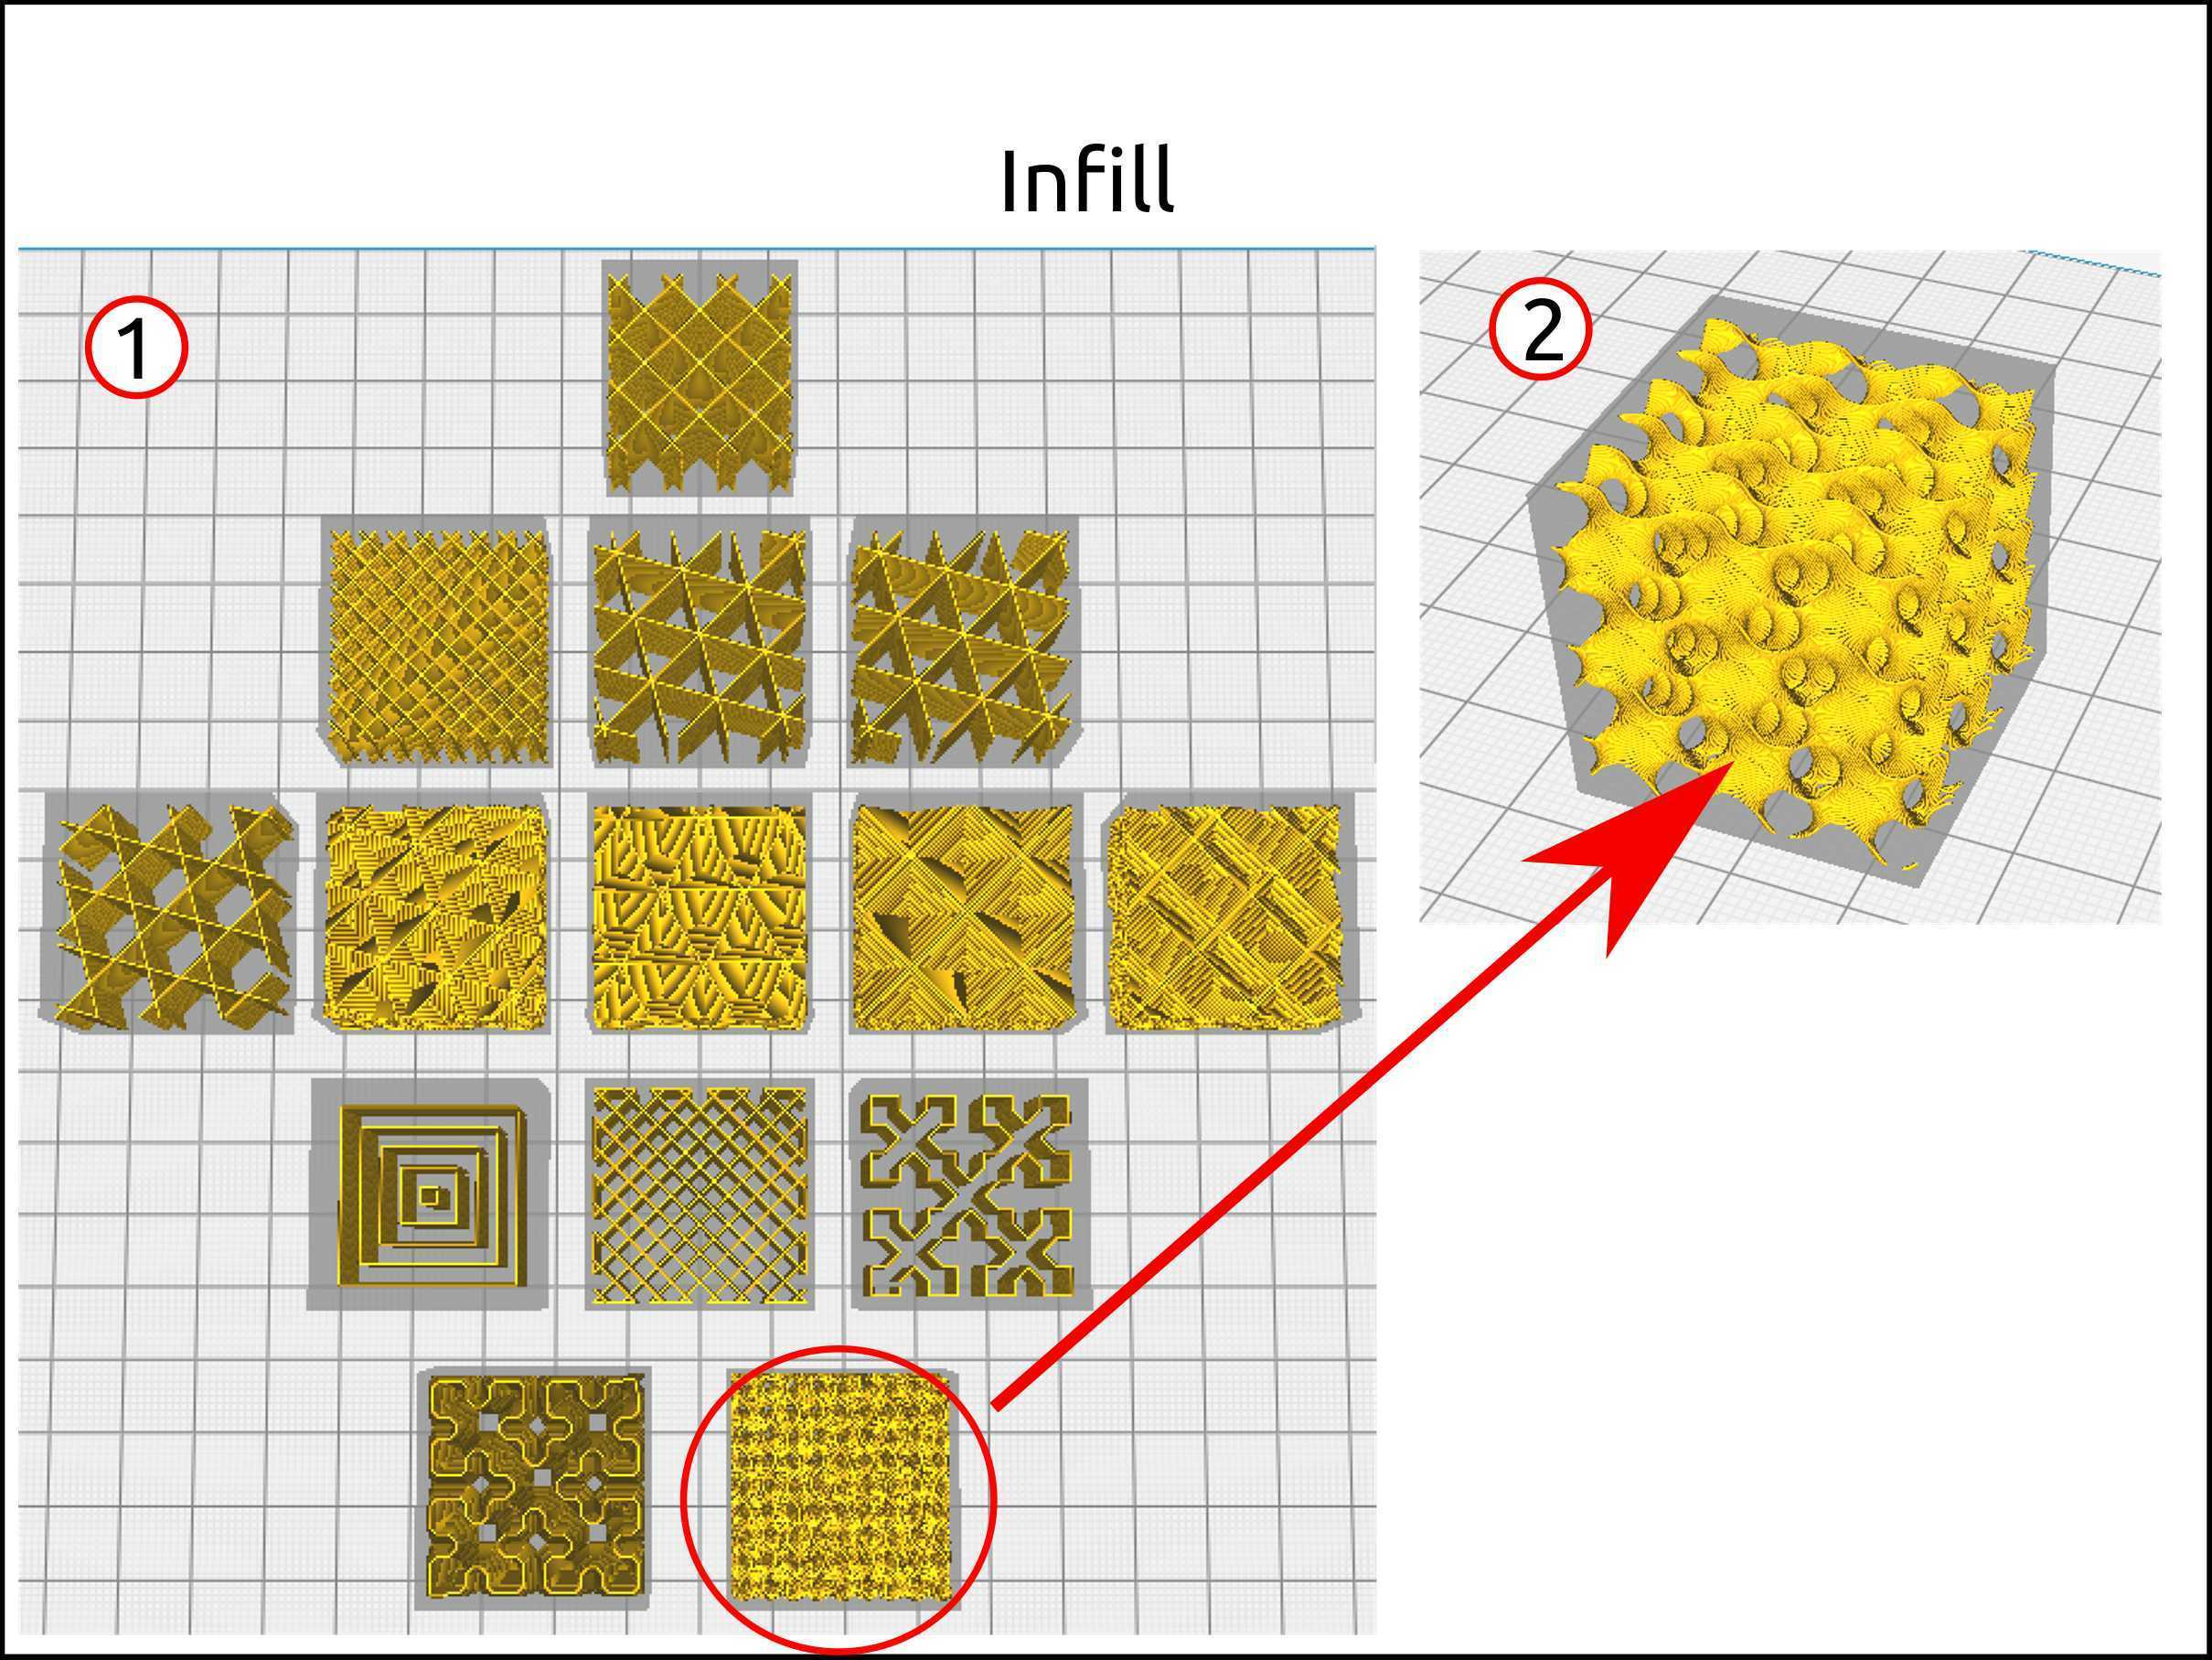
\includegraphics[width=0.5\textwidth]{chapter_2/figures/Infillbetter.jpg}
    \caption{Different types of infill \cite{UltimakerSpeed}}
    \label{fig:Infill}
\end{figure}

\subsubsection{Road orientation}
If considering roads as fibres, one would notice that the structure starts to look like a composite laminate, where one layer of unidirectional roads can be considered as a lamina. In the field of composites, lamina's and the resulting mechanical behaviour of laminates has been studied thoroughly in the book by Daniel \cite{Daniel2006EngineeringMaterials}.
Relating FFF products to composites was done as one of the first by Rodriguez et al. \cite{Rodriguez2003MechanicalModeling}, who used composite theory \ref{Modelling of FFF parts} and validated this with empirical results, as is depicted in figure \ref{fig:Orientation}.

\begin{figure}[H]
    \centering
    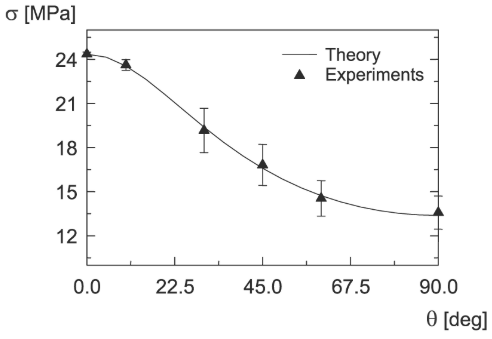
\includegraphics[width=0.4\textwidth]{chapter_2/figures/Orientation.PNG}
    \caption{Orientations of roads with respect to load applied \cite{Rodriguez2003MechanicalModeling}}
    \label{fig:Orientation}
\end{figure}

The part will have the best mechanical behaviour if it is loaded along the axis direction of the deposited roads. Subsequently, stacking the layers in  $[45/-45]_n$ configuration will result in quasi isotropic properties.

Additionally, not only the raster orientation, but the part orientation significantly influence the part properties. The printbed is in general oriented according to Cartesian coordinates, y being the longitudinal horizontal direction , y the transverse horizontal direction, and z the vertical direction (as can be seen in figure \ref{fig:coordinates}. When defining the angle of the roads, the slicers use the y direction as principle direction, meaning a [0] road will be directed along the y axis, while [90] will be directed along the x direction. 

%%% replace with ASTM F2971

\begin{figure}[H]
    \centering
    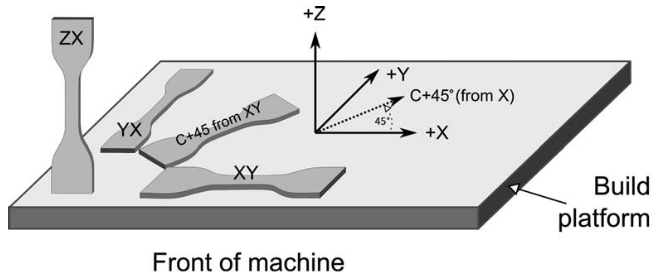
\includegraphics[width=0.4\textwidth]{chapter_2/figures/Coordinates.png}
    \caption{FFF coördinates for test specimen production}
    \label{fig:coordinates}
\end{figure}


\section{Materials}
There is currently a wide range of polymer blends available for FFF, these can also include reinforced particles. The nature of the process, liquefying the polymer, only allows for thermoplastics. Thermosets have cross-links connecting the polymer chains, causing the material to degrade rather than to flow when heated. Parameters and properties such as crystallinity, $T_m$, $T_g$ and the thermal expansion coefficient make certain polymers more applicable for FFF.  A deep comparison of different polymers and their properties will not be part of this thesis. A concise analysis and substantiation for the material that will be used in this thesis will be presented in this chapter.

\subsection{Materials for FFF}
In figure \ref{fig:pyramidpolymer} the different thermoplastic polymers can be seen. The y-axis represents the performance of the material, often related to the cost and ease of use. Be aware that the material properties of bulk or conventional produced polymer differ from the material properties found in the produced part. 

\begin{figure}[H]
    \centering
    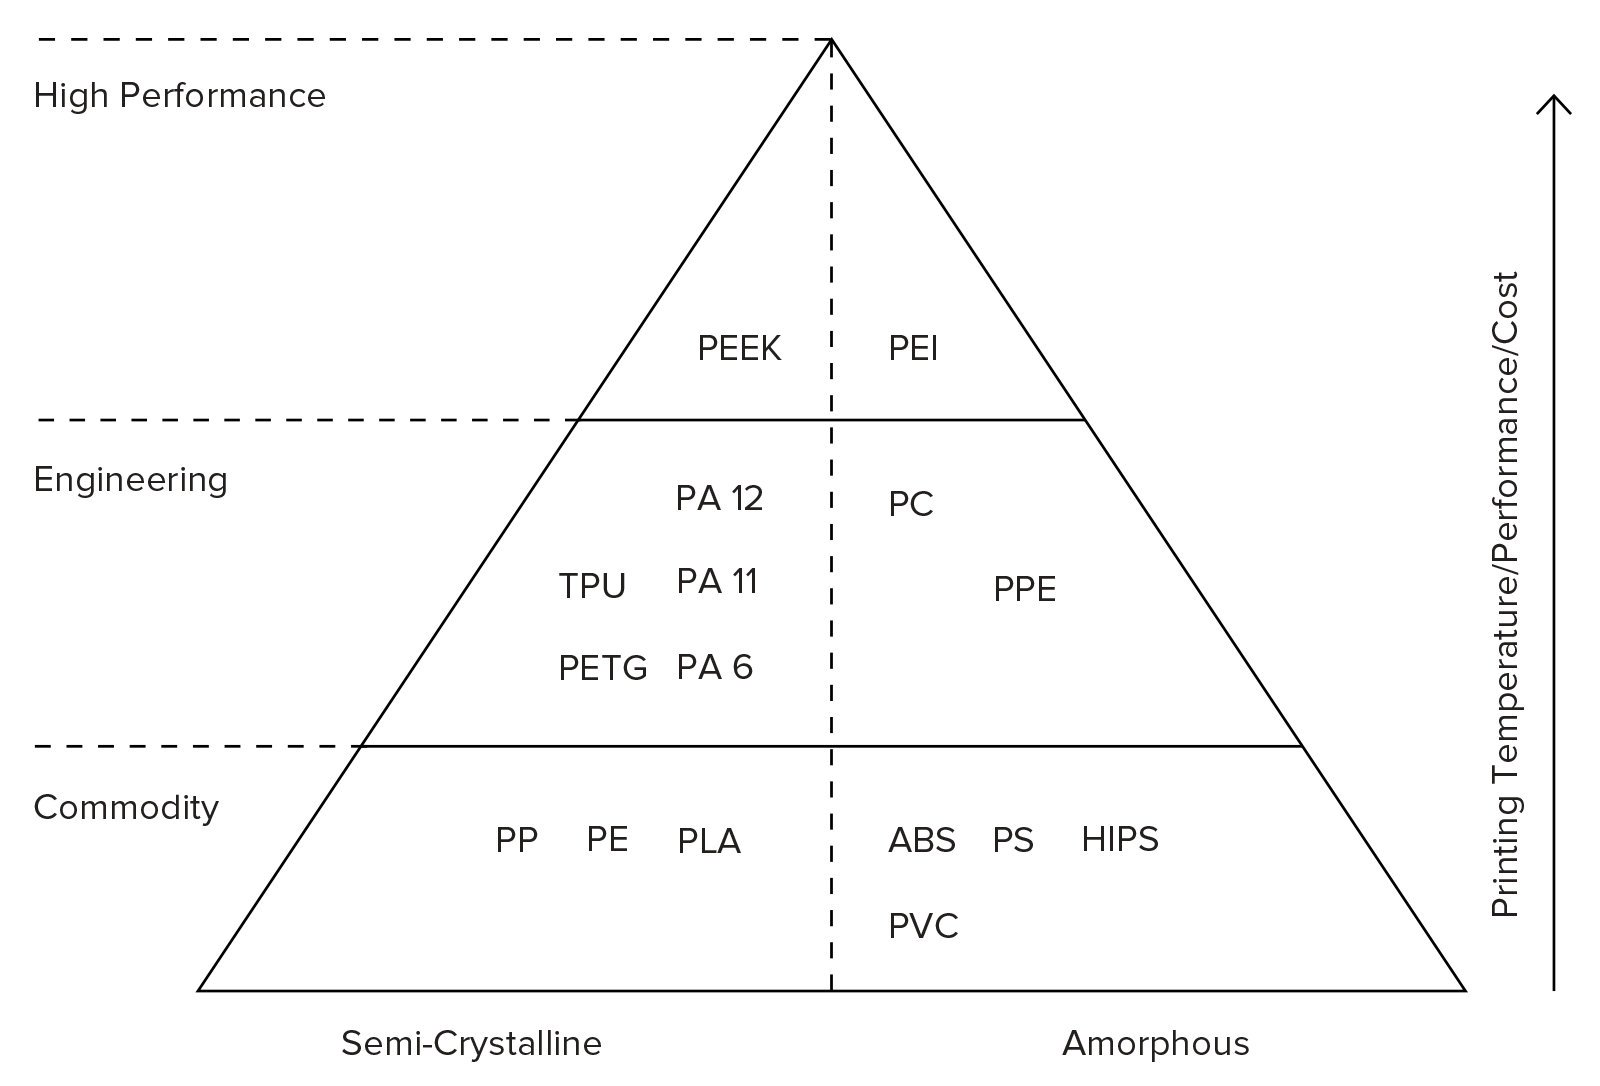
\includegraphics[width=0.6\textwidth]{chapter_2/figures/Pyramidpolymer.png}
    \caption{Polymer pyramid with FFF polymers \cite{3DHubsIntroductionPrinting}}
    \label{fig:pyramidpolymer}
\end{figure}

To create a focus for this thesis, a particular material must be chosen to apply a scope on the research. To identify the mechanical properties of FFF produced parts, and the parameters affecting this, a polymer that has been used and researched extensively should be selected. This leads us to the lower tier of the pyramid, where PLA en ABS are by far the most implemented polymers. This is mostly due to the fact that FFF printers had only the possibility to print PLA and ABS until late 2012 \cite{WohlersAssociates2017WohlersIndustry}, therefore it is not surprising that most systems are optimized for these materials. Since the academic research is limited on the topic of FFF (compared to e.g. injection moulding, which is a technology that has matured for decades), PLA and ABS are the best candidates.

PLA and ABS are most distinguishable by their polymer structure,  PLA is semi-crystalline and ABS is amorphous. This difference is mostly noticable in the thermal/viscous properties \cite{Rodriguez-Panes2018TheAnalysis}. PLA has a clear melting temperature $T_m$ (the moment where the semi-crystalline isotactic chains break its van der Waals forces), while ABS has only a glass transition temperature $T_g$, (where the polymer chains have enough thermal energy to start diffusing and consequently drop its Youngs modulus). This phenomenon is pictured in \ref{fig:EvsT}. The amount of crystallization can differ through a polymer based on the thermal history. High rates cooling can prevent chains from crystallizing, resulting in a smaller crystalline phase, this is typical for the FFF process. High degree of crystallinity is coupled with harder and thermally stable materials\cite{Balani2015PhysicalPolymers}. The amorphous regions provide elasticity and impact resistance. These properties are also reflected in the properties of PLA and ABS. The temperature history is dependant on the process parameters and geomtery, resulting in an even larger fluctuation in mechanical properties when comparing different studies. This also means that it will be harder to generate constant samples and products with semi-crystalline polymers. Additionally, Peterson \cite{Peterson2019ReviewPerspective} confirms this with the following statements; "due to the high cooling rates (in the order of 10K/s) polymers experience: 1) trapping polymers in non-equilibrium conformations; 2) limited time for polymer diffusion at road interfaces; 3) complex (in-unifromaly) crystallization profiles for semi-crysalline polymers". Crystallinity of polymers is extensively discussed in the books on polymer science by Vegt \cite{Van_der_Vegt2001FromPlastics} and Halary \cite{Halary2011PolymerMaterials}.

\begin{figure}[H]
    \centering
    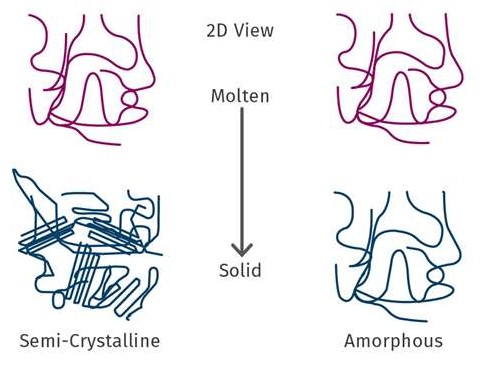
\includegraphics[width=0.3\textwidth]{chapter_2/figures/structurepolymers.PNG}
    \caption{Molecule structure in molten and solid state \cite{PtolinePolymersCrystalline}}
    \label{fig:structurepolymers}
\end{figure}

\begin{figure}[H]
    \centering
    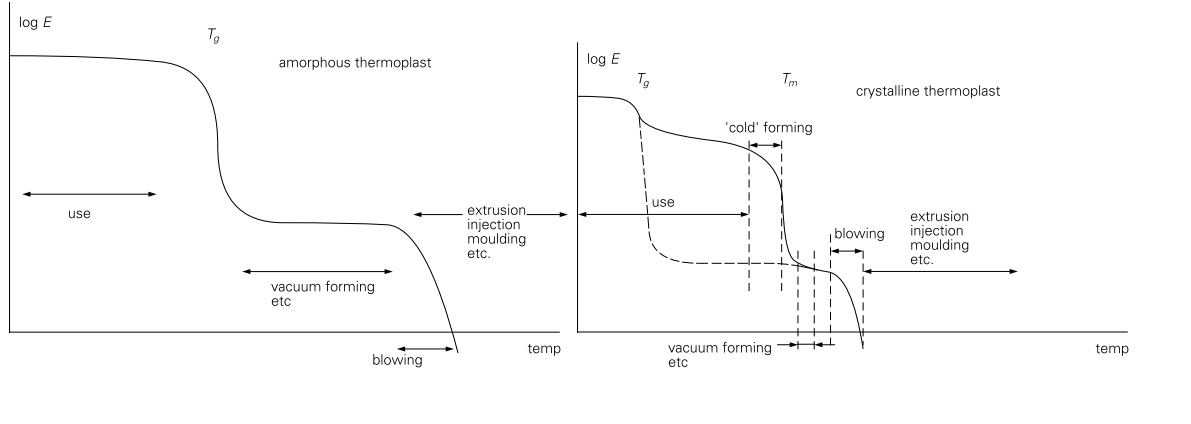
\includegraphics[width=1\textwidth]{chapter_2/figures/EvsT.PNG}
    \caption{E modulus against temperature for amorphous and semi-crystalline polymers \cite{Vegt2001FromPlastics}}
    \label{fig:EvsT}
\end{figure}

Despite that PLA is gaining popularity, due to its ease of use, low cost and biodegradability, it has limited scientific backed research compared to ABS. ABS has been used more extensively in different production methods (e.g. injection moulding). Especially with the systems of Stratasys (which were optimized for ABS P400) a lot of research was done. Popescu et al. \cite{Popescu2018FDMReview} reviewed a large amount of articles related to the mechanical properties of FFF printed parts, additionally Mohamed et al. \cite{Mohamed2015OptimizationProspects} and Peterson \cite{Peterson2019ReviewPerspective} did a similar review on the empirical research that has been done, all results are in line with previous statements.  

Taking into account the physical issues with semi-crystalline polymers and the abundance of research presented on ABS, the choice to focus this thesis on ABS is substantiated.

\subsection{ABS properties}
    \label{ABS properties}
 \subsubsection{Chemical composition}
As stated before, ABS (Acrylonitrile Butadiene Styrene $(C_8H_8)x (C_4H_6)y (C_3H_3N)z)$ is a amorphous thermoplastic with a glass transition temperature of approximately 105$^{\circ}$C \cite{Peterson2019ReviewPerspective}. Due to it's amorphous nature it has no true melting point, therefore there is no sudden viscosity drop. It is a terpolymer (build from three monomers), and is created by polymerizing styrene and acrylonitrile in the presence of polybutadiene, figure \ref{fig:ABSforumla}.

\begin{figure}[H]
    \centering
    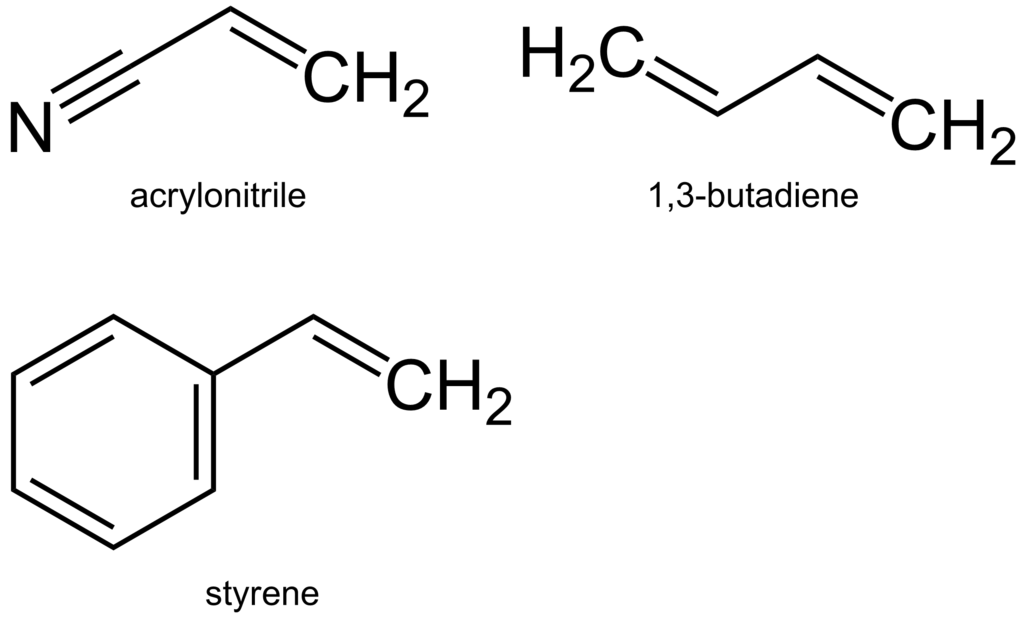
\includegraphics[width=0.\textwidth]{chapter_2/figures/ABSformula.PNG}
    \caption{Monomers in ABS polymer}
    \label{fig:ABSforumla}
\end{figure}
The proportions of the different monomers vary for Acrylonitrile from 15-35\%, which gives thermal and chemical resistance,  butadiene from 5-30\%, which gives toughness and performance over a broad temperature range and styrene 40-60\%, which is cheap, eases process-ability, machine-ability and produces high gloss \cite{GrantaDesignLimited2018CESEdupack}. This results in a long chain of polybutadiene criss-crossed with shorter chains of poly(styrene-co-acrylonitrile). ABS has a general service temperature between -30 and 70 degrees, which means that the mechanical properties in use should not differ significantly in this range. An extensive study is presented by Peterson on the ABS blends and their properties for FFF \cite{Peterson2019ReviewPerspective}.

\subsubsection{General properties}
ABS is often used due to its low cost, high impact resistance (also at low temperatures) and decent mechanical properties. It is also easy to color, is scratch and scuff resistant, and is easily processed and bonded \cite{GrantaDesignLimited2018CESEdupack}. According to CES edupack \cite{GrantaDesignLimited2018CESEdupack} general purpose extrusion ABS has low shrinkage and warpage. However, for FFF applications, ABS is difficult to use due to it's high warpage (in comparison to PLA). ABS has furthermore good resistance against chemicals and  solvents and is a decent electrical insulator. The thermal process parameters (regardless of FFF) have  effect on other properties of the ABS polymer, high temperature processes improve the gloss and heat resistance, while low temperatures increase impact resistance and strength. 
The limiting factors of ABS are its poor resistance to UV light and it's low operating temperature. The concentration of polybutadiene can increases the aging characteristics while other additives increase UV-protection. ABS is also suitable for additives such as glass and carbon fibers. 

\subsubsection{Molecular structure}
	%Reptation (healing etc)
    Thermoplastic amorphous ABS looks on a molecular scale like a spaghetti of unchained polymers, as can be seen in figure  \ref{fig:structurepolymers}. The polymers belonging to this class of materials are characterized by the temperature dependence of the Young modulus shown in figure \ref{fig:EvsT}. Each polymer chain adopts a coil conformation that strongly overlaps with its neighbors leading to chain entanglements. The entanglement density, $\nu_e$, is an important characteristic that affects the toughness of the polymer significantly, and is defined as the number of entanglements per unit volume of the material:

\begin{equation} \label{eqn:Me}
\nu_e=\frac{N_A\rho}{M_e}
\end{equation}

where $\rho$ is the polymer density, $M_e$ the molecular weight of the chain between two entanglements, $N_a$ the Avogadro number\cite{Halary2011PolymerMaterials}. 

Amorphous polymers show a significant drop in stiffness after the glass transition temperature. According to Appelsved \cite{Appelsved2012InvestigationModels}, this is the moment where the inter molecular bonds (van der Waals) break, after this moment the chains are able to diffuse through the polymer blend. 
For samples with a molecular weight higher than the molecular weight between entanglements, $M_e$, the Young modulus decreases through the glass transition and reaches a plateau value of about 1 MPa. This is called the rubberey plateau and its extent increases with molecular weight. At higher temperatures these high molecular weight polymers go trough a fluidification zone before becoming highly viscous liquids. This is consequently the phase of material where the material is extruded. If  $M$ is smaller than $M_e$, the polymer skips the rubbery plateau, and almost immediately forms a viscous liquid. A relation between the temperature molecular weight and phase is shown in figure \ref{fig:polymerphase} \cite{Halary2011PolymerMaterials}.

\begin{figure}[H]
    \centering
    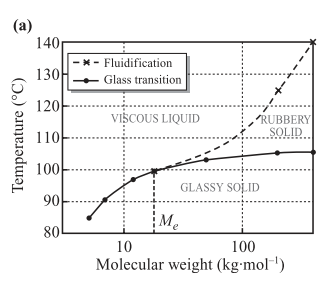
\includegraphics[width=0.4\textwidth]{chapter_2/figures/polymerphases.PNG}
    \caption{State diagram of un-cross-linked amorphous cis-1,4-polyisoprene \cite{Halary2011PolymerMaterials}}
    \label{fig:polymerphase}
\end{figure}
Reptation is possible when $M_e$ is smaller than $M$, and occurs after the glass transition temperature. The simplest form of the model assumes the polymer being "trapped" by entanglements, which is analogous to a chain trapped in a tube. The effective distance to free itself from the original entanglements is equivalent to the chain length. The speed at which the chain can reptate out of its entanglements is related to the temperature of the polymer blend\cite{Halary2011PolymerMaterials}.  
Thermoplastics inhibit inherent viscoelasticity, also called creep, which describes the phenomenon of molecule diffusion under an applied load. This mechanism is quite difficult to predict, and will not have a focus in this thesis. Most important to notice is the significant effect of the strain rate on the mechanical response of thermoplastics, as is shown in figure \ref{fig:Strainrate}
When extruding or processing thermoplastics, chains are being broken and reduced in length, this decrease in molecular weight leads to alteration of the response under different temperatures as is shown in \ref{fig:polymerphase}.

% Mechanical behaviour
\subsection{Elasticity}
Polymers exhibit an elastic response to a loading that is defined as instantaneous and reversible and may have either an energetic or an entropic physical origin. These constitutive mechanism are designated as true elasticity and hyper elasticity respectively. True elasticity, which for polymers only occurs at low strains, is linked to a poisson ratio that varies between 0.3 at low temperature and 0.5 at temperatures equal to or higher than the glass transition temperature. 
The entropic effect describes the increase in entropic energy (heat) of the polymer chain as a larger force due to the dynamic movement of the molecule. 
Random coils can be considered as a spring, multiple springs are connected to each other through entanglements. Thermosets, which contain crosslinks, have more predictable elastic behaviour than thermoplastics, which inhibit a large amount of viscoelasticity. However, these entanglements have similarities to cross links in the glassy state at a low strain, these enthanglements will dissapear as a result of sliding motion of the chain. Different models exists to predict the elastic behaviour of polymers, especially for thermosets, these are defined in detailed in the book of Halary \cite{Halary2011PolymerMaterials}. If we consider the stress strain curve of a typical thermoplast from figure\ref{fig:SSpolymers}, we observe a quasi-linear region up to the top of the curve where $d\sigma/d\epsilon=0$. This top is defined as the yield point for thermoplastics \cite{Afd2016NEN-EN-ISO527-2}, which differs from the definition for e.g. metals. According to Appelsved \cite{Appelsved2012InvestigationModels} the true yield point of polymers is the stress at which van der Waals bonds are all broken, and chains can diffuse freely.  

\begin{figure}[H]
    \centering
    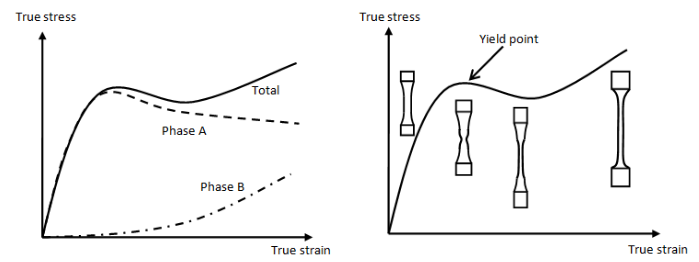
\includegraphics[width=0.6\textwidth]{chapter_2/figures/SSpolymers.PNG}
    \caption{Typical stress-strain curves for thermoplastics \cite{Appelsved2012InvestigationModels}}
    \label{fig:SSpolymers}
\end{figure}
Additionally, Appelsved differentiates two different phases (figure \ref{fig:SSpolymers}); phase A which dominates up to the stress maxima and deformation is mainly generated from movement of the molecular chains relatively to each other. Eventually the bonds break and the slope decreases. Since a polymer blend is a distribution of chains with different lengths, this is expected to occur over a strain range instead of a sudden drop. After the bonds are broken strain softening occurs. In phase B, the molecule chain itself is straightened, resulting in re-hardening at larger strains. The alignment at large strains cause transverse isotropy. The straightening of the molecular chains makes the material stronger, resulting in a different necking behaviour in contrast to metals. 

\begin{figure}[H]
    \centering
    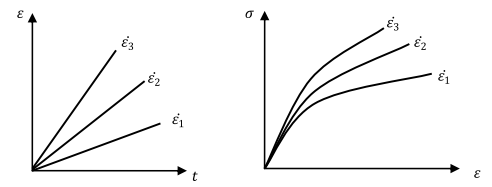
\includegraphics[width=0.5\textwidth]{chapter_2/figures/Strainrate.PNG}
    \caption{Effect of strain rate dependency on polymers \cite{Appelsved2012InvestigationModels}}
    \label{fig:Strainrate}
\end{figure}
\subsection{Plasticity, damage and failure}
Due to the molecular structure of polymers, it is difficult to determine the start of plasticity. Loading/unloading experiments can be carried out to determine irreversible strains.  The effect of loading and un-loading is depicted in figure \ref{fig:Irr}. The unloading is followed by recovery, until the residual strain have stabilized and can be concluded as permanent.
\begin{figure}[H]
    \centering
    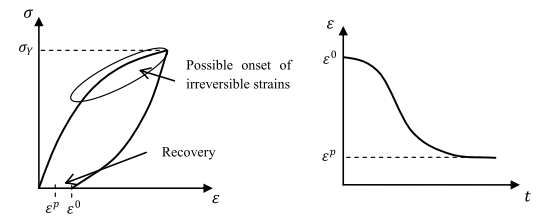
\includegraphics[width=0.5\textwidth]{chapter_2/figures/Irr.PNG}
    \caption{Loading/unloading behaviour with recovery \cite{Appelsved2012InvestigationModels}}
    \label{fig:Irr}
\end{figure}
Halary \cite{Halary2011PolymerMaterials} claims that conducting compressive tests have the advantage of avoiding the effect of micro-voids always present in samples, since these voids increase sample brittleness on straining. In figure \ref{fig:SSPMMA} empirically generated uniaxial compression stress strain curve of an amorphous thermoplastic polymer (PMMA) can be seen. The slope of the straight line corresponds to the material Young modulus. Between A and B the stress-strain relation is no longer linear and the material exhibits an anelastic behaviour. In figure \ref{fig:SSresidual} a schematic drawing of different loading regions is shown to support the explanation. In this region strain is still reversible. After the stress maximum at the yield point, a clear viscoplastic behaviour occurs. Additional strain is irreversible, and will lead to residual strain after unloading. It is worth pointing out that these residual strains can be removed by heating the polymer sample above its glass transition temperature. In general, it can be assumed that the Youngs modulus remains relatively similar up to the plastic range. 

\begin{figure}[H]
    \centering
    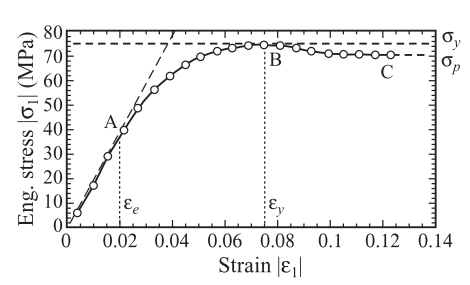
\includegraphics[width=0.5\textwidth]{chapter_2/figures/SSPMMA.png}
    \caption{Compression stress-strain curve of a PMMA (A, elastic limit; B,yield point; C, plastic flow)\cite{Halary2011PolymerMaterials}}
    \label{fig:SSPMMA}
   \end{figure}
\begin{figure}[H]
    \centering
    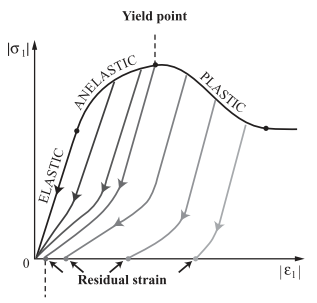
\includegraphics[width=0.4\textwidth]{chapter_2/figures/SSresidual.png}
    \caption{Schematic drawings of unloading profiles for a sample compressed at various strain values.)\cite{Halary2011PolymerMaterials}}
    \label{fig:SSresidual}
   \end{figure}
%\subsubsection{Yielding}
\subsubsection{Yielding}
%\subsubsection{Dependency on Hydrostatic stress (models)}
Most common yield and failure criteria, like von Mises and Tresca \cite{Christensen2013TheFailure}, are dependent on the stress state of the material. This stress state is a function of the von Mises ($\sigma_v$) or equivalent stress:

\begin{equation}\label{von mises}
\sigma_v=\sqrt{\frac{(\sigma_{11}-\sigma_{22})^2+(\sigma_{22}-\sigma_{33})^2+(\sigma_{33}-\sigma_{11})^2 +6(\sigma_{23}^2+\sigma_{13}^2+\sigma_{12}^2)}{2}} 
\end{equation}


However, these do not include dependency on the hydro-static stress, which is most common for metals. Yield and failure criterion for polymers are generally dependant on the the hydrostatic stress ($\sigma_h$):
\begin{equation} \label{eqn:Me}
  \sigma_h=P=\frac{\sigma_x+\sigma_y+\sigma_z}{3}
\end{equation}
Additionally the yield and failure are criterion are a function of the the stress triaxiality ($\sigma_t$):
\begin{equation}\label{AzziTsai}
\sigma_t=\frac{\sigma_h}{\sigma_v}
\end{equation}
The difference in yield and failure loci can be observed in figure \ref{fig:yieldloci}
\begin{figure}[H]
    \centering
    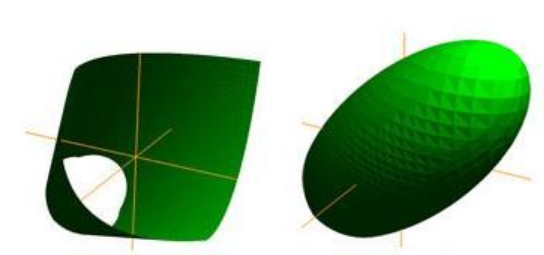
\includegraphics[width=0.5\textwidth]{chapter_2/figures/yieldloci.png}
    \caption{Failure locus for metals (left), and for ductile polymers (right), with the axis corresponding to the principle directions \cite{Christensen2013TheFailure}}.
    \label{fig:yieldloci}
\end{figure}
The axis in this figure represent the principle stress directions. The left surface is defined by a stress state of the von Mises stress. If a pure hydrostatic pressure is applied, the surface will not be crossed. For polymers there is also a dependency on the hydro static pressure, since it  will cross the surface at some point.  
It should me mentioned that the yield and failure surface for polymers is in reality not symmetric for tension and compression, as can be seen in figure \ref{fig:SStensioncompression}. It has been concluded by several book on fracture mechanics \cite{Janssen2014Co-magmeasurewD.pdf} that polymers have a higher compressive yield strength than in tension. 
For ductile polymers also failure criteria are used based on the equivalent strain. This strain is calculated in a similar way as the equivalent stress. The failure surface might differ from the conventional von Mises or Tresca surfaces. 
\begin{figure}[H]
    \centering
    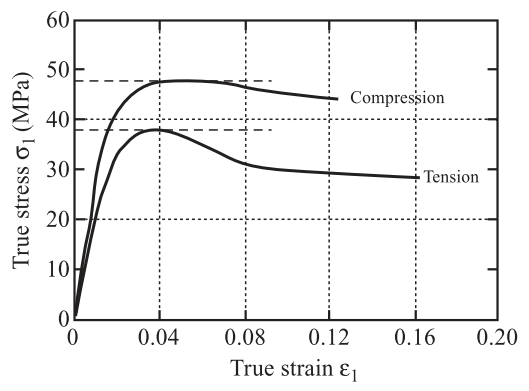
\includegraphics[width=0.3\textwidth]{chapter_2/figures/SStensioncompression.png}
    \caption{Comparison of stress-strain curves for PMMA for compression and tension \cite{Halary2011PolymerMaterials}}
    \label{fig:SStensioncompression}
\end{figure}

Assuming a isotropic polymer blend of ABS, we need to define a yield function based on the principal stress state of the material, $f(\sigma_1,\sigma_2,\sigma_3)$ that is also dependant on the on the hydrostatic pressure. 
Claiming that a material has hydrostatic pressure sensitivity permits us to write the stress tensor as the sum of its deviatoric $\sigma_p$, and volumetric stress (the identity matrix multiplied with the hydrostatic stress) components, as expressed in equation \ref{eqn:deviatoric}:
\begin{equation}\label{eqn:deviatoric}
\begin{vmatrix}
\sigma_{1}&0&0\\
0&\sigma_{2}&0\\
0&0&\sigma_{3}\\
\end{vmatrix}
=
\begin{vmatrix}
\sigma_{1}-P&0&0\\
0&\sigma_{2}-P&0\\
0&0&\sigma_{3}-P\\
\end{vmatrix}
+
\begin{vmatrix}
P&0&0\\
0&P&0\\
0&0&P\\
\end{vmatrix}
= \sigma_d+\sigma_h*I
\end{equation}Where $I$ is the identity matrix.  
An enhanced form of the von Mises criterion can then be applied to polymers in the following way:
\begin{equation} \label{eqn:yieldpolymers}
  (\sigma_{11}-\sigma_{22})^2+(\sigma_{22}-\sigma_{33})^2+(\sigma_{33}-\sigma_{11})^2=(2\sigma_y+\mu_{vM}*\sigma_h)^2
\end{equation}
Where $\mu_{vM}$ is an internal friction coefficient. The corresponding plasticity envelope is a cone whose axis is the hydrostatic pressure axis, and whose axis increases with hyrdrostatic pressure, similar to the yield locus for polymers in figure \ref{fig:yieldloci}. A similar procedure can be applied to the tresca criterion. 

\begin{figure}[H]
    \centering
    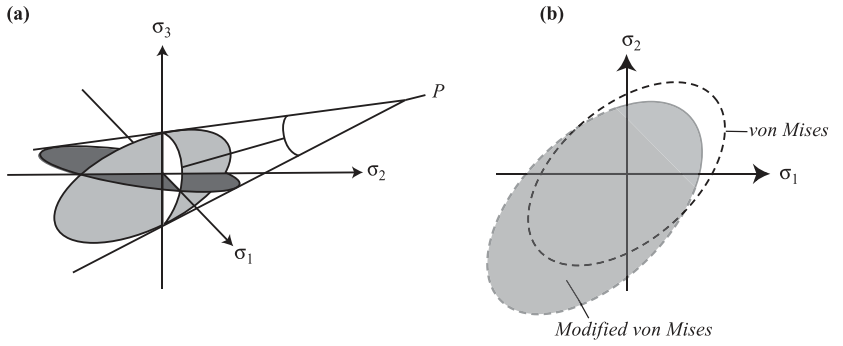
\includegraphics[width=0.75\textwidth]{chapter_2/figures/yieldpolymers.png}
    \caption{Yield surface for polymers a) three-dimensional b) two-dimensional compared with von Mises \cite{Halary2011PolymerMaterials} }
    \label{fig:Midplane}
\end{figure}

%Ree-Eyring
The Ree-Eyring model explains the yield behaviour on a molecular scale, according to this model, the sliding of molecules with respect to each other is achieved by passing through a transition state, called activated state, overcoming an energy barrier depending on both temperature and applied stress. This models assumes plastic deformation of amorphous polymers is occurs as the displacement of chain segments from a site A to a site B due to an activation state, related to energy $\Delta G$, both located in a sliding plane resulting from the presence of a shear component. The principle of the model can be seen in figure \ref{fig:Ree-Eyring}. In the anelastic range the chains are merely "stretched" and will not permanently displaced with respect to the other chains in the blend. In comparison with the theory presented by Apselveld, one could argue that the "activation energy" for permanent displacement is analogous to the breaking of the van der Waals bonds.

\begin{figure}[H]
    \centering
    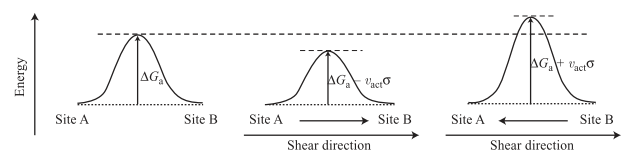
\includegraphics[width=0.8\textwidth]{chapter_2/figures/Ree-Eyring.png}
    \caption{Energy diagram showing the principle of the Ree-Eyring model \cite{Halary2011PolymerMaterials}}
    \label{fig:Ree-Eyring}
\end{figure}
%plastic instability
During tensile tests beyond the yield point many polymers, including amorphous polymers, undergo a plastic instability, the necking phenomenon. In this plastic region, chains have reached their extensibility limit, further neck propagation occurs trough neighboring regions. After development of the whole neck propagation a uniform strain occurs again, until the sample breaks as can be seen in figure \ref{fig:Necking}. In figure stable necking is observed, while in figure b unstable necking leads to quick fracture. This behaviour depends on the considered polymer, possible defects, temperature and strain rate conditions. 
\begin{figure}[H]
    \centering
    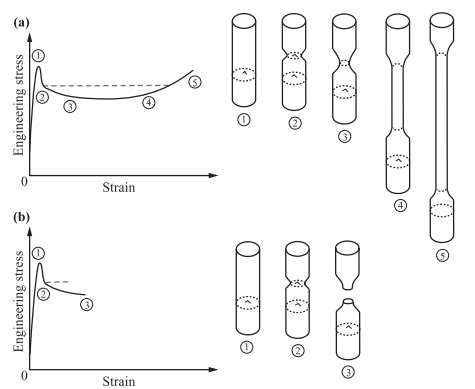
\includegraphics[width=0.4\textwidth]{chapter_2/figures/Necking.png}
    \caption{Schematic drawing of the necking phenomenon \cite{Halary2011PolymerMaterials}}
    \label{fig:Necking}
\end{figure}
There exists several yield and failure criteria for thermosets and composites. Since thermpolastics have a more complex behaviour due to their viscoeleasticity in this section the different models will be discussed. 
Lin\cite{Lin2013StressLoading} confirms the lack of accurate yielding and failure criteria for thermoplastics. Additionally, the PhD. thesis of Melick \cite{Melick2002DeformationGlasses} on the deformation and fracture of polymer glasses also mention the lack of failure criterion, and does not produce a satisfying solution for tis issue. Different  models (brittle or ductile) are implemented in commercial software sucha as the equivalent strain criterion, von Mises, Johnson-Cook, Hill and Drucker-Prager. The main drawback in these fracture models is that accurate predictions of failure can only be achieved for limited stress state and strain rate, which cannot be applied for thermoplastics. One of the currently popular material models for polymer plasticity  in LS-DYNA is SAMP-1 (semi analytical model for polymers)

Melro \cite{Melro2013MicromechanicalModelling} proposes a paraboloidal yield criterion for epoxies defined by Tschoegl, which can be defined as:
\begin{equation}\label{eqn:Tschoegl}
\Phi=6J_2+2I_1(\sigma_c-\sigma_t)-2\sigma_c\sigma_t
\end{equation}Where $J_2$ is the second invariant of the deviatoric stress tensor, and $I_1$ = tr(\textbf{$\sigma$}). This is a variation of the general yield criterion shown in equation \ref{eqn:yieldpolymers}

Du Bois \cite{DuBois2006APolymers} implemented a seminanalytical model for the simulation of polymers (SAMP-1) in LS-DYNA under MAT187. 
\begin{equation}\label{AzziTsai}
f=\sigma_v^2-A_0-A_1*\sigma_h-A_2*p^2<0
\end{equation}For further details the reader is referred to the mentioned article. 

Another popular yield criterion that is used by the SAMP-1 material model in LS-DYNA is that Drucker-Prager yield criterion. 

\subsubsection{Damage and failure}
Damage and fracture are important to investigate to identify the failure mechanism of the polymer, both concepts cannot be dealt with separately, since fracture, which results in the sample breakdown, usually comes after damage. Depending on the deformation conditions (stress field, temperature, strain rate) and characteristics of the polymer chains (chemical structure, molecular weight), two types of deformations may occur: shear bands and crazes. Shear bands are deformations in shear direction (45 degrees for uniaxial compression tension), important to note is that they do not create any voids inside the material, and therefore will not induce and volume change. Shear band growth is controlled by plastic sliding only, therefore, stress associated with shear band formation is assumed to be equal to the yield stress. 

%crazes
Crazes are small microvoids containing fibrils bridging the two craze faces. Such fibrils play a major role in the ability of the craze to sustain loading in the direction perpendicular to its faces. These microvoids are ellipsoidal heterogeneities with a size ranging from 10 $\mu$m to 10 mm along the major axis and from 1 to 10 $\mu$m in along the minor axis. In figure \ref{fig:Craze} a schematically image is shown of crazes. The ratio between crazes an fibrils are approximately equal.  

\begin{figure}[H]
    \centering
    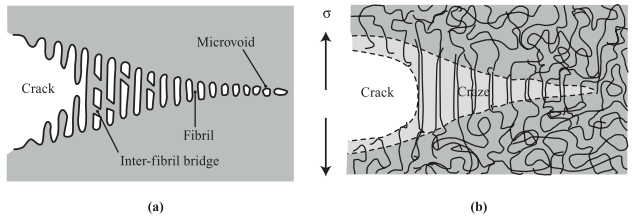
\includegraphics[width=0.8\textwidth]{chapter_2/figures/Craze.png}
    \caption{Schematic drawing of a craze a) Microvoids b) conformations of chains within a craze \cite{Halary2011PolymerMaterials}}
    \label{fig:Craze}
\end{figure}
A crack systematically initiates from a sample "defect". Despite a crack being inherently different from a craze, a craze initiates from microvoids. These defect lead to stress concentrations allowing the craze to grow, but only at temperatures under the glass transition temperature. These stress concentrations can be predicted by conventional fracture mechanics, but are outside the scope of this thesis. Fibrils in the crazes may either break, which requires to break high energy covalent bonds, or when undergoing higher mobility, may slide with respect to each other. The first results when high strain rate is applied at low temperature, and the latter occurs at a  temperature near $T_g$. These mechanisms occur under tension at a stress lower than yield stress, and grow perpendicularly to the direction of the highest principle stress.
A craze criterion is proposed based on two arguments:
- Crazes are formed when strain reaches a critical value, $\epsilon_c$, along one direction.
- This strain craze value, which varies with temperature and strain rate, depends on the hydrostatic component of the stress tensor according to:
\begin{equation} \label{eqn:crazecriterion}
 \epsilon_c=Y+\frac{X}{\sigma_1+\sigma_2+\sigma_3}
\end{equation}
%adding strain surface??
Where X an Y are experimental parameters. From this criterion a envelope can be made to compare it with the von Mises yield criterion as can be seen in figure \ref{fig:crazecrit}. 

\begin{figure}[H]
    \centering
    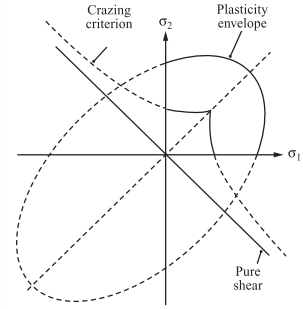
\includegraphics[width=0.3\textwidth]{chapter_2/figures/crazecrit.png}
    \caption{Plasticity envelope and craze criterion for PMMA \cite{Halary2011PolymerMaterials}}
    \label{fig:crazecrit}
\end{figure}

The craze strain criterion can occur before yielding and plasticity, whereas shear bands only occur beyond the plasticity threshold. This result implies that any combination of two tensile stresses generates crazes instead of shear bands. A combination of a tenisle and compressive stress might lead to both, pure compression always generates shear bands.
To discriminate between shear bands and crazes, one could perform optical microscopy. Extensive research was conducted on this topic, the general conclusions are that the type of damage (crazing or shear bands) are dependant on the polymer, stress state, and temperature. In amorphous thermoplastics, both can be identified by the whitish color due to the scattering of light trough polymer alignment. This effect is more intense for crazing, as a result of the higher density, and is more localized for shear banding.
Additionally interactions may exist between these two types of damage. Initiation of shear deformation zones at the craze tip can occur when the craze propagation rate and widening are small. 

Halary et al. concluded that despite the issues with microvoids, the uniaxial tensile test and uniaxial compressive tensile have a generally identical shape and domains. Fracture occurs in the viscoplastic domain, it is a ductile fracture with a specific angle of about 45 degrees between the fracture line and stretching direction. At lower temperatures, fracture generally takes place in the anelastic domain, there might be overlap with theory concerning brittle fracture of metals at low temperatures.  

In FEM modelling software different damage and failure models are implemented. The damage initiation point defines start of degradation of stiffness, it only leads to effective damage if damage evolution is specified \cite{ABAQUS2006MaterialFailure}. In case of ductile damage, D is a function of plastic straining and affect the yield stress rather than the elastic modulus. This is equivalent to plastic softening. The material point is assumed to fail when the overall damage variable D reaches a critical value $D_{max}$.
A general form of the strain based fracture loci for thermoplastics can be written as follows
\begin{equation}\label{AzziTsai}
\bar{\epsilon_f}=f(\eta)=f(\frac{\sigma_h}{\sigma_v})
\end{equation}
%In the SAMP-1 a simple damage model was added where the damage parameter D is a function of plastic strain only. In this model a load cuve must be provided by the user giving D as a function of the plastic strain under uniaxial tension. The value of the critical damage $D_c$ leading to rupture is then the only other required additional input, this model behaves istropically. Furthermore the model uses the notion of the effective cross section, which is the true cross section of the material minus the cracks that have happened. 
%This models assumes the start of damage from the yield point, and fails when the damage parameter D drops to 0.   

Where $\bar\epsilon_f$ is the equivalent strain at failure. 
%maybe implement equivalent strain here
One of the most popular fracture and damage models for polymers is the Johnson Cook model, widely implemented in ABAQUS and LS-DYNA softaware:

\begin{equation}\label{AzziTsai}
\bar\epsilon_f=(D_1+D_2*exp{(D_3*\frac{\sigma_h}{\sigma_v})}*(1+D_4*\frac{\dot{\epsilon}}{\dot{\epsilon}})
\end{equation}
Where $d_i$ are material parameters\cite{BoisA:}, the Hancock-McKenzie approach defines the following parameters: $d_1=0, d_2=3/2, d_3=\epsilon_{1f}*exp(-1/2)$. Additionally, a paper by Gao \cite{Gao2013CriticalPipelines} proposes a different variant of the Johnson Cook criterion:

\begin{equation}\label{eqn:JC}
\bar\epsilon_{f}=1.65\epsilon_{1f}{(-\frac{3}{2}*\frac{\sigma_h}{\sigma_v})}
\end{equation}Where $\epsilon_{1f}$ is the critical strain for ductile materials at which crack are initiated under tension in one direction. Different strain based failure criteria are proposed in LS-DYNA and abaqus. Most implement a simple plastic strain at failure ($\epsilon_p<\epsilon_{pf}$) or a major strain failure ($\epsilon_1<\epsilon_{1f}$), and others use the Johnson-Cook criterion as is described.  

Damage in combination with the Johnson Cook model is defined in material model SAMP-1 in LS-DYNA as:

\begin{equation}\label{AzziTsai}
D=\epsilon_p/\epsilon_f\Rightarrow D<D_c\Rightarrow\epsilon_p<\epsilon_{pf}=D_c*\epsilon_f
\end{equation}The influence of stress triaxiality in a strain based failure criterion is important because different states of stress would result in a different equivalent strain at failure\cite{BoisA:}. 
%damage in polymers
A damage variable, denoted as D, quantifies the part of the material cross section that no longer transmits forces (cracks or voids). In the following, only isotropic damage is considered. Elastic damage affects material stiffness, ductile damage affects material strenght or both material strength and stiffness. This depends on the chosen formulation where two different approaches may be postulated: strain equivalence or energy equivalence. We will be discussing strain equivalence in this section. 

Damage in polymers is relatively hard to model, since different mechanisms play a large role in the determination of damage. A study on the damage behaviour of polymers \cite{Gu2013ExperimentalThermoplastics}, Gu et al. presents different damage functions based on literature and proposes damage functions based on experimental data. 
The general stiffness damage as function of plastic strain is defined as

\begin{equation}\label{stiffnessdamage}
E_{eff}=E_0*(1-D)
\end{equation}Where Nutini and Vitali proposed a simple definition of the damage parameter calculated from the volume strain, since an important characteristic of thermoplastics is the generation of damage (voids and crazes) during plastic volumetric deformation $\epsilon_v$, which is defined as the sum of the principle strains.

\begin{equation}\label{AzziTsai}
D=1-exp(-\epsilon_v)
\end{equation}

In figure \ref{fig:damagepolymer} the results from a loading/unloading experiment was carried out on a polypropylene sample to get more insight on the damage behaviour. 

\begin{figure}[H]
    \centering
    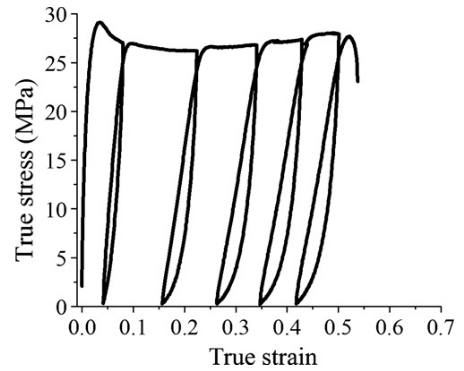
\includegraphics[width=0.4\textwidth]{chapter_2/figures/damagepolymer.png}
    \caption{Sample of trues stress-strain curve of polypropylene\cite{Gu2013ExperimentalThermoplastics} }
    \label{fig:damagepolymer}
\end{figure}
As can be seen, the Youngs modulus slightly decreases with plastic strain. However, after the first cycle (just after the softening region) the change in stiffness seems minimal.  Unfortunately, no absolute values of the Youngs moduli are presented in this study. 
Following the results, this study proposed a damage function that follows the equation \ref{eqn:stiffnessdamage} fitting the experimental results. Since the damage only occurs in the plastic region for polymers, the result is a function of plastic strain ($\epsilon_p$), and is fitted with a double term exponential function:

\begin{equation}\label{AzziTsai}
D=A*(exp(B*\epsilon_p)-exp(D*\epsilon_p))
\end{equation}The study concludes that the damage parameter calcultated with the volumetric deformation underpredicts the damage occurring. A possible reason is that besides voids and crack that might be captured with the volumetric strain, microscracks that do not lead to macroscopic volume change also contribute to damage. 

Christensen \cite{Christensen2013TheFailure}  published a detailed book on failure criteria, but did not take into account materials that exhibit strain softening, therefore his extensive work can unfortunately not be used. 

Rodriguez \cite{Rodriguez2003MechanicalModeling} investigated yield modelling for composite materials under multi-axial loading. He implemented a theory proposed by Tsai-Hill for composites, which is an extension of the von-mises yield criterion, which defines failure for composites. Originally the Hill theory was developed for anisotropic ductile and brittle materials. Different variations are used for either failure or yield criteria. The  surface is assumed to be quadratic in the stress components. Details on these yield criteria can be found in books on composite mechanical behaviour \cite{Daniel2006EngineeringMaterials}, \cite{Mallick2007Fiber-Composites}.

\subsubsection{Fracture}
Another failure approach is the study of fracture in cracked surfaces. Among the three opening modes, I requires the smallest stress to propagate the notch, therefore, it is considered as the most destructive mode and is often used to estimate the material toughness. A sample weakened by a notch and or crazes will exhibit a lower Youngs modulus, therefore, the stress at break, $\sigma_b$ is lowered. On the opposite $\sigma_y$ is only slightly modified. Classical fracture theories can be implemented for crack growth and fracture, these assume a thick plate with a crack of length $2a$. An approach that combines Irwin Criterion and  the approach of Griffith is that a sharp crack can propagate within an finite sample under a critical stress:

\begin{equation} \label{eqn:criticalstress}
 \sigma_{cc}=\frac{K_{Ic}}{\sqrt{(\pi*a)}}
\end{equation}
Where $K_{Ic}$ is the critical stress intensity for mode 1 loading. This relates the value of the local stress intensity in the surroundings of the crack tip to the applied loading and is dependant on the material and geometry of the crack. 

The  $K_{Ic}$ has a correlation with the material energy release rate, $G_{Ic}$ under plane strain state, involving the Young modulus and the poisson ratio according to: 

\begin{equation} \label{eqn:crazecriterion}
K_{Ic}=\frac{E*G_{Ic}}{\sqrt{1-v^2_p}}
\end{equation}
Irwin was the first to take into account that stress concentrations at the crack tip may be large enough to move from a local elastic to a plastic response. 

\begin{figure}[H]
    \centering
    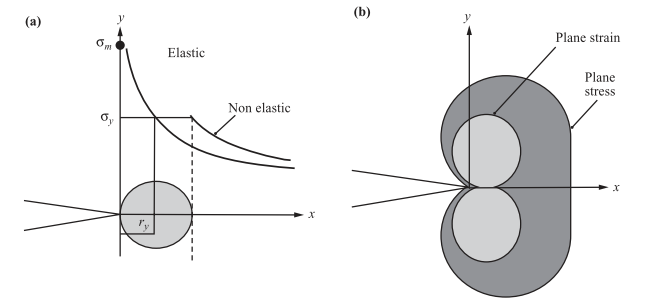
\includegraphics[width=0.4\textwidth]{chapter_2/figures/Crackstress.png}
    \caption{Geometry of the plastic zone a crack tip a) Irwin model b) analysis using von Mises stress\cite{Halary2011PolymerMaterials}}
    \label{fig:stresscrack}
\end{figure}
The radius of the plastic region, $r_y$, as is shown in figure \ref{fig:stresscrack} has been modeled by Irwin under plane strain with the following dependency:

\begin{equation} \label{eqn:cracktip}
r_y=\frac{1}{6\pi}*\left(\frac{K_I}{\sigma_y}\right)^2
\end{equation}There are different ways to calculate $K_{Ic}$ and  $G_{Ic}$, this thesis will not go into detail to determining these values. These values are dependant on numerous polymer characteristics, such as chemical structure, molecular weight, glass transition temperature, etc. It should be noted that the values shift with the thickness of the specimen and is significantly higher for plane stress than for plane strain. Therefore, this method is less appropriate for parts not consisting of plates. 
%Molecular approach of fracture behviour.
Chain entanglements play a fundamental role in fracture properties. Correlations between the fracture properties of polymers and their entanglement density, $v_e$ where found by Halaray et al., as can be seen in figure \ref{ref:KIc}.  

\begin{figure}[H]
    \centering
    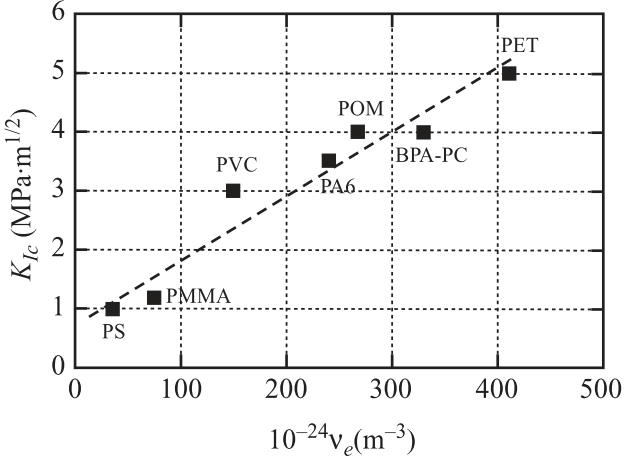
\includegraphics[width=0.4\textwidth]{chapter_2/figures/KIc.png}
    \caption{Correlation between toughness, $K_{Ic}$, and entanglement density, $v_e$  \cite{Halary2011PolymerMaterials}}
    \label{fig:stresscrack}
\end{figure}
These empirical results shows that there is a linear dependence  between the two factors as would be predicted by theory. 

Unfortunately, the work of Halary et al. does not include investigations on ABS polymers. 
%Hergenhahn \cite{Hergenhahn2002FractureABS} has investigated the fracture toughness of ABS for different thicknesses. Following the Izod procedure, the fracture toughness of ABS was found to be 2.8 $MPa*m^{-3/2}$ and for a thickness of 15 mm 2.77. 
Oskui \cite{Oskui2014ExperimentalDevice} determined a fracture toughness of 4.32 $MPa m^{-3/2}$ for a 10 mm thick specimen. %others also had 4. 

%these analytical models might be appropriate for our problem, but the goal of this thesis is to implement and validate a numerical model, therefore they will not be researched further. 

\subsection{Application of ABS for FFF}
\label{Application of ABS for FFF}
Due to its low glass transition temperature, it's ease of processability, low cost and decent mechanical properties, ABS is a popular polymer to be used for FFF printing of functional parts. Since PLA is even cheaper and easier to use, this polymer is generally used for prototyping and aehstetical parts. Polymers such as PETG, PC and PA are generally used for functional parts. When printing without a heated chamber, polymers with high $T_g$ (for PC 147$^\circ C$) will loose a significant part of their properties due to bad bonding. ABS has a relatively high glass transition temperature ($T_g$ 105), PETG ($T_g$ 80$^\circ C$) and PA ($T_g$ 60$^\circ C$) will have less issues with this. What causes difficulty for the use of ABS with FFF is warping. Coating the build surface with an adhesive will significantly reduce warping.


%the curling of the part (which especially happens for large areas touching the buildplate). This is due to the shrinkage of the first layers that are attached to the bottom layer, this causes the bottom layer to be pulled from the buildplate. To ensure that the part adheres well to buildplate it is essential to have a calibrated "leveled" bed (which determines the distance between the extruder and the buildplate). Also a heated build plate can be incorporated, which drastically limits the thermal gradient between the first layers, reducing thermal stresses. Over cooling the parts with the fans or convection will make your part more prone to warping. A brim (a small entourage of extra roads around the part) is also helpful to stop the part from warping. 
%The extent of warpage is mostly related to the thermal expansion coefficient, $\alpha$, which is around 120 $\mu m/(m C^{\circ}$) according to CES edupack. Even though warpage is an essential part of producing functionally viable parts, it will not be part of this thesis. In future work in this thesis, warpage will not be taken into account. 
It is important to note that the parts produced with FFF are weakest at the inter-laminar interface, and that in different loading conditions the parts most certainly will fail at the laminar interface \cite{Hart2018IncreasedAnnealing} \cite{Popescu2018FDMReview}

\subsection{Standard parameters for ABS}
    \label{standard parameters for ABS}
The technical data sheet of ABS produced by Ultimaker \cite{Ultimaker2018TechnicalABS} assumes the "fine" settings in Cura. These include a 0.4mm nozzle printed at 240-250 C and has a build plate temperature of 85 C, additionally it has a printing speed of 55 mm/s. These settings are recommended for an optimal print, the amount of infill orientation and shell architecture is up to the judgment of the producer. Automatically the slicer produces a shell of about 3 roads thick and applies an infill of 20-50\% filled with a triangle structure. Due to differences in parameters, difference in material and system, lack of standardization, qualification and characterization of results, the produced parts by different researchers will differ widely. Therefor it is difficult to compare the different empirical results from different researchers and datasheets. E.g., the UM datatsheet only states that the printed test specimen are printed in 90\% infill, but the orientation, geometry of the infill and additional parameters have a crucial influence on the mechanical properties of the part. 

\subsection{Standardization}
    \label{Standarization}
In the prior sections it has been made clear that there are a wide range of parameters that can be adjusted. However, there is limited guidance in the standardization of the production process to produce a procedure that can be reproduced. Different researchers have tried to create standardization for their work, generating a multitude of different parameters that are being used, this is well portrayed by review studies such as \cite{Peterson2019ReviewPerspective} and \cite{Popescu2018FDMReview}.  Most plastic producers give relatively little to no information on the process parameters used to test their filament, as can be observed in the Ultimaker ABS datasheet \cite{Ultimaker2018TechnicalABS}. One of the most important characteristics that fluctuate in parts being produced (even if the same process parameters are used), is the healing, wetting and porosity in parts. Although the wetting and porosity can be analyzed by observing the mesostructure, it is extremely hard to characterize the extent of polymer entanglement that will result in road bonding. Employing good hardware (such as a constant envelope heater), reliable sensors and thermocouples and high quality robotics and stepper-motors will generate more consistent results. After a part is produced it can be checked trough some relatively easy steps to determine the quality as described by Tanikella et al. \cite{Tanikella2017TensilePrinting}, e.g. one can weight the produced part to create an estimation for the porosity, and to determine the fluctuation in extrusion by comparing it with the calculated weight by the slicer. Additionally, one could perform a density test by applying the Archimedes principle.

In the past years efforts have been made to use standard printing processes and test procedures.. Nist \cite{Forster2015NISTApplicability} published a standard for testing additively manufactured polymer materials, including FFF thermoplastic testing. These test methods advise using either ISO 527-2 \cite{Afd2016NEN-EN-ISO527-2} or ASTM D638 \cite{Materials2015ASTMD638-14} for tensile test, which both describe the tensile test for a thermoplastic polymers. They are similar on most points, indicating a geometry and test conditions for the experiments, including a sample size of 5 specimen per test. In general this seems like a decent test method, however, in some cases (due to the large in-isotropic behaviour and nonuniform bonding between roads) the test specimen fails in unexpected ways, often failing at the clamps or the fillets due to stress concentrations\cite{Alaimo2017InfluenceParts}, or having consecutive roads failing due to bad layer bonding and surface roughness \cite{Ahn2002AnisotropicABS} \cite{Bertoldi1998MechanicalDeposition}. 

As an alternative to the ISO 527 or ASTM D638 standard, a composite alternative is proposed by Rodriguez \cite{Rodriguez2001MechanicalInvestigation}, which applies the ASTM D3039 on his tests, which are normally used for long fiber samples. The advantage of this standard is the fact that it does not have fillets at the end of the sample, reducing the stress concentration and possibility for defects.

The document presented by NIST \cite{Forster2015NISTApplicability} still lacks standars on the production of test specimen. Additionally, ISO and ASTM published useful documents on general principles and terminology including ISO 17296  \cite{Afd2014NEN-EN-ISO179-1} ISO/ASTM 52900 \cite{ASTMInternational2017ISOParts} ISO/ASTM 52901 \cite{2019NEN-EN-ISOParts} ISO/ASTM 52910  \cite{ASTMInternational2017ISOParts} ISO /ASTM 52921 \cite{Nen-iso2019NEN-EN-ISOTestmethoden} ASTM F2971 \cite{2013ASTMManufacturing}, the last standard assumes a coordinate system (figure \ref{fig:coordinates}) which will be used for further reference. A book on standards and quality control was presented by Chua et al. \cite{ChuaStandardManufacturing}

Rodriguez \cite{Rodriguez2003MechanicalModeling} has assumed three normal material directions in line with the Chauchy stress tensor to simplify the reference to the road structure as can be seen in figure \ref{fig:Principlematerial}. This is in accordance with the notation for orthotropic materials such as long fibre composites.
\begin{figure}[H]
    \centering
    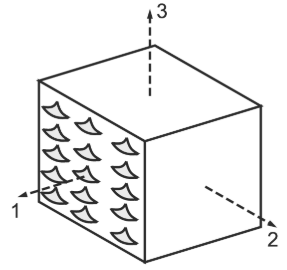
\includegraphics[width=0.25\textwidth]{chapter_2/figures/Principlematerial.PNG}
    \caption{Three principle directions in the axis of asymmetry}
    \label{fig:Principlematerial}
\end{figure}

If one were to produce test specimens, the convention states that the orientation of the test specimen has two directions which define the orientation of the test specimen, the first being the direction of the longest side of the specimen, the second being the smaller side. In figure \ref{fig:coordinates} the coordinates for sample production are defined. 
To define the direction of the roads (the raster orientation) one could look at the slicer software used (in this case Cura) which defines the deposited road orientation at the angle [0] to be in the Y direction (therefor [90] is in the X direction). Multiple papers use different orientation systems which can be quite confusing and ambiguous. To be consistent and easily comprehensible, this convention will be used throughout this thesis. This will be important when referring to orientations and tested samples in rest of the report. 

After damage or delamination of a layer or a set roads, the properties of the part change, which create a difficult situation to model. H.Li et al. \cite{Li2002CompositeProperties} have developed numerical approaches that uses composite theories including multi-state of elastic, softened and de-bonded state.  Since these are complicated and strongly dependant on the process parameters, these will not be further discussed here. 

%Tanikella, Nagendra G Interesting graph here
%TNO rapport Julius Berens

\section{FFF properties}
    \label{chp:FFF properties}
We have concluded that the process parameters largely influence the properties of FFF produced parts and are dissimilar from conventional produced counterparts. It is made clear that the products from this process create significant anistropy resulting in orthotropic parts (three mutually perpendicular planes of symmetry), porosity, weak layer/road interfaces and surface roughness and inconsistencies. The benefits from FFF produced parts are the geometrical freedom, almost negligible start-up cost due to the absence of a mall or expensive machinery, relatively fast production, integration of different parts without the need of joining and for Defence applications; the large logistic freedom to create parts in remote area's.

\subsection{Experimental mechanical characterization}
Conducting experimental tests with constant process parameters and 100\% infill in the three general directions (as is shown in figure \ref{fig:Principlematerial}) will give more insight in the mechanical behaviour of FFF products. The notation of the produced samples in the 3 directions are respectively; YX[0] direction 1, XY[0] direction 2 and ZY[0] direction 3. The properties that will govern their behaviour will be consecutively; the axial road properties (intra fiber properties), the horizontal (adjacent, inter fiber properties) road bonding, the vertical (stacked, inter fiber properties) layer bonding. This theory is supported by different papers including work done by Alaimo \cite{Alaimo2017InfluenceParts}

Intuitively, the YX[0] specimen would generate the best behaviour, since there are no bonds in the direction of the load. Montero \cite{Montero2001MaterialExperiments} concluded that the bond between layers in shear is stronger and stiffer  than between roads. They also did a tensile test including horizontal specimen with transverse and axially aligned rasters, the results of his stress strain graphs are shown in figure \ref{fig:Transverseraster}. 

\begin{figure}[H]
    \centering
    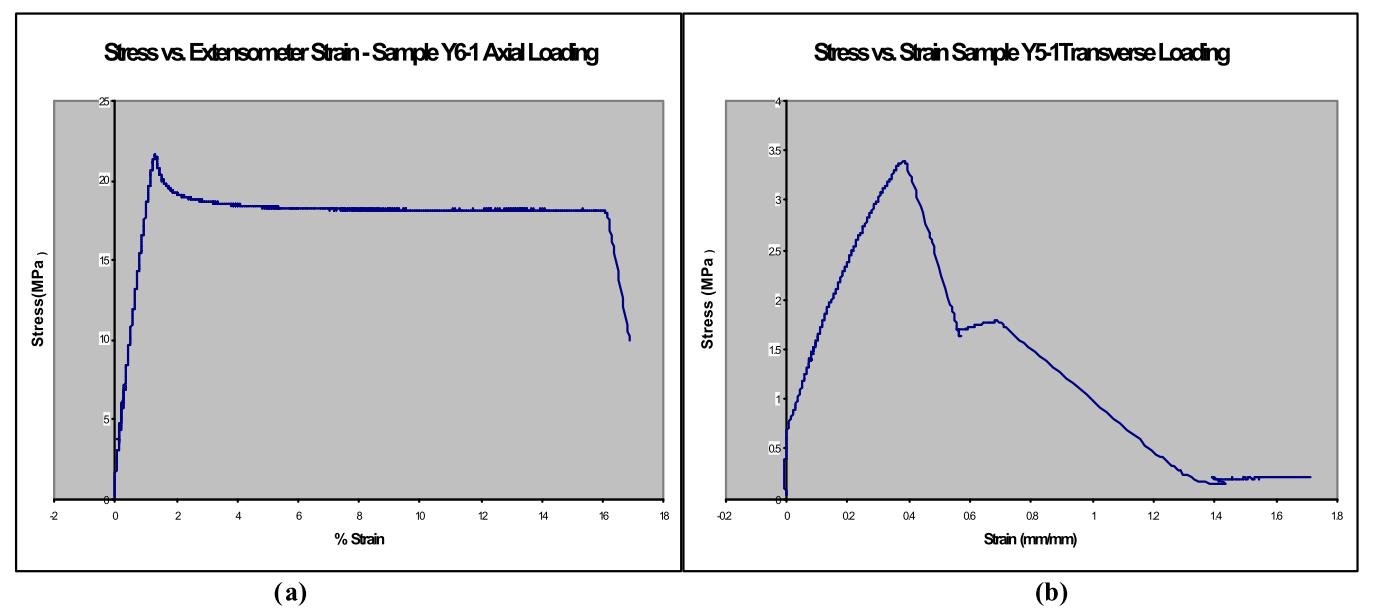
\includegraphics[width=0.7\textwidth]{chapter_2/figures/Transverseraster.PNG}
    \caption{a) (YX)[0] b) (XY)[0] \cite{Montero2001MaterialExperiments}}
    \label{fig:Transverseraster}
\end{figure}

Multiple researchers did similar research, which is limited to the research of the raster orientation in the horizontal plane. This lacks to obtain the information concerning the layer bonding ZY[0]. Roderiguez et al. were probably one of the first to analyze the mechanical behaviour of different FFF orientations, they provide a clear graph (figure \ref{fig:Rodriguezgraph}) comparing the results with bulk ABS \cite{Rodriguez2001MechanicalInvestigation}. This graph clearly suggests an almost linear elastic region with a perfect plastic response for the longitudinal direction and a linear elastic brittle behaviour for the transverse directions. 

\begin{figure}[H]
    \centering
    \includegraphics[width=0.5\textwidth]{chapter_2/figures/Rodriguezgraph.jpg}
    \caption{stress strain graph for (YX)[0] (long.dir.) and (XY)[0] \cite{Rodriguez2001MechanicalInvestigation}}
    \label{fig:Rodriguezgraph}
\end{figure}

Without knowing the exact behaviour of the ZY[0] test (3 direction), we can predict (using the properties stated in the TDS of Essentium \cite{EssentiumTechnicalPLA} that it might respond similar to XY[0] but with a lower yield (and UTS) point. However Essentium indicates that the flexural properties of a XY[0] sample are worse than ZY[0]. Montero indicates shear in XY[0] is also worse. Be advised that these experiments are made with different settings and materials, so no conclusions could be made before obtaining comparable data. Blok \cite{Blok2018AnComposites} indicates that the stiffness can be 11\% lower and tensile strength up to 50\% lower in the XY[0] and ZY[0] direction compared wity the YX[0] direction. 

Rodriguez \cite{Rodriguez2001MechanicalInvestigation} also tested the filament and additional features such as crazing and necking. Localized whitening of the specimen has been observed before the yield stress was reached. Failure occurred at whitened areas where localized fiber delamination occurred, these white areas can also be caused by shear bands. He concluded that crazes propagate much faster along the bonding regions than they do in the ABS bulk due to the low interface strength. When loading in the axial direction of the roads there is a small amount of necking observed \cite{Garg2017AnStudy}, which is in line with the stress-strain curve of figure \ref{fig:Rodriguezgraph}. Since crazes are formed due to the plastic deformation induced by polymer stretching, crazing at interroad bonds should suggest a high degree of polymer entanglement.

One of the last things to mention about the result of FFF parts is the assumption of the thermal residual stresses induced by the process. Since they show visco-elastic behaviour at room temperature, one would suggest that the chains would relax over time towards a relaxed state. It has been shown \cite{Veen2019EnhancingTemperature} that thin walled polymer samples with a low $T_g$ will relax its chains after a period of time resulting in a strain in the z direction. %%%%%%%%%%%%%%%%%%extra reference???% 

Annealing and post processing has been discussed to some extent in academic literature (e.g. by Thomas and Rodriguez \cite{Thomas2000ModelingRoads}).

%Constitutive law Domingo, H Li, Bertoldi, Montero, Alaimo, Knoop

%\subsubsection{Road bonding}
%Rodriguez

%(already discussed to some extent)

%\subsubsection{direction}

%Can add math model part of H. Li to thermal analysis and bonding strength
%(already discussed)

%Mechanical behaviour structure, H. Li (very nice paper)

\subsection{Mesostructure}
\label{mesostructure}
The mesostructure of a FFF part (the road structure on 0.1 to 1 millimeter scale) characterizes a significant amount of the mechanical properties of the FFF produced part. It was already discussed that the laminate-like nature of the FFF parts resembles composites. Multiple studies \cite{Somireddy2017MechanicalMesostructure} \cite{Somireddy2018DevelopmentFDM} \cite{Rodriguez2001MechanicalInvestigation} were conducted to characterize the mesostructure by microtoming, a process to cut micrometer thick slices of a specimen, this procedure will be further discussed in chapter 4. Afterwards the sample is inspected with optical microscopy and a digital image is produced. This procedure is used in different scientific fields and has been adopted for the inspection of the cross section of FFF samples. A few, among which Enrique Cuan-Urquizo \cite{Cuan-Urquizo2019CharacterizationApproaches} (\ref{fig:SEMmesostructure}) and Ahn \cite{Ahn2002AnisotropicABS} \ref{fig:AhnMeso}observed the mesostructure (\ref{fig:SEMmesostructure}) with SEM (scanning electron microscope) which gives a more detailed perspective on the mesostrucure, but might be too expensive and time-consuming for multiple investigations.

% extra citations \cite{Rodriguez2003MechanicalModeling} \cite{Rodrguez2003DesignStrength} \cite{Sun2008} \cite{Patanwala2018TheComposites} \cite{Li2017TheProperties} \cite{Sheth2017NumericalOrientation} \cite{Li2002CompositeProperties}


The fundamental mesostructure (cross section of XY[0] specimen) is a structured stacking of multiple roads in a rectilinear cadence. If standard extrusion settings are implemented with a well calibrated system, the FFF system should deposit a road structure similar to the one seen in figure \ref{fig:Meso10&20} b. As has been discussed in the section \ref{Process parameters}, the process parameters have a large influence on the result on the mesostructure.  The mesostructure could be optimized (meaning a decrease in porosity) by increasing the flow multiplier.

\begin{figure}[H]
    \centering
    \includegraphics[width=0.5\textwidth]{chapter_2/figures/SEMmesostructure.PNG}
    \caption{Mesostructure observed with SEM by Cuan-Urquizo} \cite{Cuan-Urquizo2019CharacterizationApproaches}
    \label{fig:SEMmesostructure}
\end{figure}

\begin{figure}[H]
    \centering
    \includegraphics[width=0.5\textwidth]{chapter_2/figures/AhnMeso.jpg}
    \caption{Mesostructure observed with SEM by Ahn} \cite{Ahn2002AnisotropicABS}
    \label{fig:AhnMeso}
\end{figure}

These micrographs give an abundant amount of information on the road structure, wetting, necking and the amount of porosity in a part. This type of characterization is essential to determine the quality of the parts and the consistency of the process. Different systems, parameters and materials have influence on the results of the mesostructure. There is also a common consensus in these studies that the degree of polymer bonding (and consequently weld strength) are a function of the temperature and time of the contact area between two roads. Although, there is not a common agreement on the form of the roads nor the connection to the process parameters and the degree of overlap. The roads are interpreted as different forms by different academici, including ellipses, ovals and oblongs. Someriddy \cite{Somireddy2018DevelopmentFDM} and Sun \cite{Sun2008} assume ellipses in their work, the disadvantage is that the overlapped material is not accounted for. 
It is difficult to make a good assumption concerning the form of the roads in the mesostructure, since the form is largely influenced by the process parameters and other non-controllable process phenomena which  result in a relatively complex form. The reason of characterizing the road form is to be able to model the geometry of the mesostructure in a FEA for the prediction of mechanical properties. This will be further discussed in chapter 5. 
%this is good

%A different approach is followed by the Slic3r manual written by Hodgson \cite{GaryHodgsonSlic3rMath} where he explains how the extruded material of the roads is calculated. In his model he assumes a stadium shaped road, which is also supported by Patanwala \cite{Patanwala2018TheComposites} Additionally to the conclusions found in the section about road width, Hodgson claims that with a higher line width the bonding in the z direction would be better due to a larger contact area and consequently a lower amount of porosity. He explains how the Slic3r software assumes stadium shapes instead of ellipses as is shown in figure \ref{fig:Slic3rshape.png}. 
%The area according to Hodgson is therefore calculated as following: 
%\begin{equation} \label{eqn:crazecriterion}
%A=(w_e-h)*h+\pi(h/2)^2
%\end{equation}
%Where $h$ is the nominal layer height and $w_e$ is the extruded line width. 
%diameter, the excess line width (which was expected to be 10\% by Somireddy) becomes 50\%(!). The micro graphs and single lines produced are in line with the 10\% theory, however the tolerance tests gave results that the parts to be fitted have a over dimension of 0.3-0.4 in 2 directions, resulting in a 75\%-100\% increase in line width, which would actually be closer in line with the Hodgson theory.


%\begin{figure}[H]
    %\centering
    %\includegraphics[width=0.5\textwidth]{chapter_2/figures/Slic3rshape.png}
    %\caption{Road shape calculated by the slic3r shoftware \cite{GaryHodgsonSlic3rMath}}
    %\label{fig:Slic3rshape.png}
%\end{figure}

%The ratio between the nominal line width and the nominal layer height is recommended to be around 2, and is not recommended to drop below 1.  
%With this shape a void area is found with this equation:
%\begin{equation}
%A_v = h ^2 - (h/2)^2 * \pi
%\end{equation}
%And the void fraction can be found with
%\begin{equation}
%f_v = \frac{A_v}{A}
%\end{equation}
%He proposes an overlap factor (from 0 to 1) to find the optimum for filling in the void area's, the overlap factor represents how much void remains between the extrusions. It's difficult to estimate this amount, since it also depends on viscosity of plastic, extrusion speed and temperature. To generate enough material to fill in these voids an overlap between two layers should be calculated that encompasses exactly the voids between roads. The equation for the overlap between roads become 
%\begin{equation}
%\delta l = h* (1 - \pi/4)
%\end{equation}
%And additionally,
%\begin{equation}
%w_e = w+\delta l
%\end{equation}

%If considering roads with nominal width of 0.4  and 0.2 heigth, the extrusion width will be 0.44, which is exactly in line with the observations of Somireddy.  

%When creating an alternating raster the mesostructure will obviously be affected. The most common laminates that generate the largest amount of istropy are (YX)[0/90]n and (YX)[45/-45]n, which create laminates that are perpendicular to each other. Hongbin \cite{LiHongbin2017TheProperties} has analysed the (YX)[45/-45]n structure thoroughly. Important to take into account for the prediction of mechanical properties is the different contact areas between layers, since there is no matrix there is a limited contact surface that bonds layers. 

%THINK ABOUT THIS PART
%For regular (YX)[0]n structure the contact area for one road reference to figure \ref{fig:Mesostructurestructure}, is 2x in y direction and 2z in z direction which is continuous in the x direction. 
%%make equation for contact points determined by width and height
%Therefor, if we extrude the road for length w, the contact area of one road would be $((2x)+(2z))*2*w=4(x+z)*w$. However, considering $YX[45/-45]_n$, the contact area of one unit cell of $w*h*w$ would be $(2z)*2*w+2x*2x=4z*w+4x^2$, but since $w>2x$ the resulting contact area will always be smaller than the contact area of $YX[0]_n$.

%A good understanding of the mesostructure can give a better understanding of the mechanical properties of a part when combined with computational models such as Finite Element Analysis (FEA) which could be used to compare the numerical simulation with empirical test to analyze the effect of the polymer orientation on the mechanical properties of a part.

\section{Composite theory}
    \label{Modelling of FFF parts}
Since it was concluded that FFF parts are an-isotropic and have particular mechanical behaviour due to it's process, it is difficult to predict the properties of such parts. Therefore, it would be beneficial if these properties were possible to model, so the parts could be implemented based on the prediction from the models. 

\subsection{Elastic modelling}
\subsubsection{Stiffness in orthotropic materials}
As has been discussed in the section \ref{chp:FFF properties} we can conclude that the layers are thin and behave as orthotropic material, and therefor, orthotropic constitutive relation for plane stress case can be considered, a similar approach has been found in multiple papers \cite{Rodrguez2003DesignStrength} \cite{Rodriguez2003MechanicalModeling} \cite{Somireddy2018DevelopmentFDM} 
%\cite{Somireddy2017FlexuralStudy} \cite{Somireddy2017MechanicalMesostructure} \cite{Li2017TheProperties} \cite{Ahn2002AnisotropicABS} \cite{Alaimo2017InfluenceParts} \cite{Sheth2017NumericalOrientation} \cite{Patanwala2018TheComposites}. 

The stress strain relation for an orthotropic body can be written in the contracted notation as

\begin{equation}\label{eqn:compliancematrix}
\begin{vmatrix}
\sigma_{11}\\
\sigma_{22}\\
\sigma_{33}\\
\sigma_{12}\\
\sigma_{23}\\
\sigma_{13}\\
\end{vmatrix}
=
\begin{vmatrix}
C_{11}&C_{12}&C_{13}&0&0&0\\
C_{21}&C_{22}&C_{23}&0&0&0\\
C_{31}&C_{32}&C_{33}&0&0&0\\
0&0&0&C_{44}&0&0\\
0&0&0&0&C_{55}&0\\
0&0&0&0&0&C_{66}\\
\end{vmatrix}
\
\begin{vmatrix}
\epsilon_{11}\\
\epsilon_{22}\\
\epsilon_{33}\\
\epsilon_{12}\\
\epsilon_{23}\\
\epsilon_{13}\\
\end{vmatrix}
\end{equation}Since this matrix is diagonally symmetric, the amount of elastic constants is reduced to 9.

Plane stress is achieved by defining $\sigma_{33}$=0 $\sigma_{23}$=0 $\sigma_{13}$=0. The compliance matrix $|C|$ written becomes:


\begin{equation}\label{eqn:compliancematrix}
\begin{vmatrix}
\epsilon_{11}\\
\epsilon_{22}\\
\epsilon_{12}\\
\end{vmatrix}
=
\begin{vmatrix}
\frac{1}{E_1} & \frac{-v_1_2}{E_1} & 0\\
\frac{-v_{12}}{E_1} & \frac{1}{E_2} & 0 \\
0 & 0 & \frac{1}{G_{12}}\\
\end{vmatrix}
\
\begin{vmatrix}
\sigma_{11}\\
\sigma_{22}\\
\sigma_{12}\\
\end{vmatrix}
\end{equation}

The stresses and the stiffness matrix $|Q|$ can be acquired by inverting equation \ref{eqn:compliancematrix} resulting in 

\begin{equation}\label{Stiffnesmatrix}
\begin{vmatrix}
\sigma_{11}\\
\sigma_{22}\\
\sigma_{12}\\
\end{vmatrix}
=
\begin{vmatrix}
\frac{E_1}{1-v_1_2v_2_1} & \frac{-v_1_2E_2}{1-v_1_2v_1_2} & 0\\
\frac{-v_1_2E_2}{1-v_1_2v_1_2} & \frac{E_1}{1-v_1_2v_2_1} & 0 \\
0 & 0 & G_1_2\\
\end{vmatrix}
\
\begin{vmatrix}
\epsilon_{11}\\
\epsilon_{22}\\
\epsilon_{12}\\
\end{vmatrix}
\end{equation}

The resulting independent material constants, $E_1, E_2, v_{12}$ and $G_{12}$ are needed to determine what the mechanical response of a thin FFF product would be.

\subsubsection{Mechanics of Materials}
The mechanics of materials approach is based on simplifying assumptions of either uniform strain or uniform stress in the constituents. These predictions are adequate for longitudinal properties such as Young's modulus $E_1$ and major poisson's ratio $v_{12}$. These properties are not sensitive to fiber shape and distribution, this approach underestimates the transverse and shear properties\cite{Daniel2006EngineeringMaterials}

\subsubsection{Rule of mixtures}
The rule of mixture (ROM) is a commonly used principle in the application of composites, when two different materials are combined in a solid, the ROM can combine the different material properties to predict the new solid characteristics. When loading a composite ply in the 1 direction (along the fibre axis), the elastic properties can be predicted with the parallel or Voigt model\cite{Daniel2006EngineeringMaterials} 

\begin{equation} \label{eqn:Voigt}
E_1=V_f*E_{1f}+(1-V_f)*E_1_m
\end{equation}

Where $E_1$ is the elastic modulus of the ply in direction 1, $V_f$ is the fibre volume and $V_m$ is the matrix volume. Following this formula, and considering the ABS roads as $V_f$ and the porosity as $V_m$, one could predict the elastic properties in the 1 direction by obtaining the void density in the 1 plane.

The different approach can be used for loads in the transverse (2) and (3) directions. The model used for composites is called series of Reuss model \cite{Daniel2006EngineeringMaterials} 

\begin{equation} \label{eqn:Reuss}
E_2=\frac{E_{2f}*E_{2m}}{(E_{2f}*V_m+E_{2m}*V_f)}
\end{equation}
However, this takes a few rough assumptions, since the cross section of the voids are not continuous in the 2 and 3 directions in contrast to the 1 direction, it will be more difficult to determine the void density in the 2 and 3 directions. 

Li et al. \cite{Li2002CompositeProperties} proposes an equation to account for transverse stiffness:

\begin{equation} \label{eqn:ROMseriesfactor}
E_2=\zeta(1-\rho_2)*E
\end{equation}
where $\zeta$ is an empirical factor that takes into account the bonding strength. $\rho_2$ is a linear void fraction along the transverse direction. $1-\rho_2$  represents the relative contact area of the neck between roads. The void area density is determined according to empirical observations. 

Rodriguez \cite{Rodriguez2003MechanicalModeling} proposed a method to obtain the the $E_1$ and $E_2$ where he calculates the cross sectional void density to be squared voids with perfect bonding. He additionally assumes the void density to be uniform in any given plane trough the solid. 
\begin{equation}\label{eqn:E_1}
E_1=(1-\rho_1)*E
\end{equation}The void area density in the 2 direction is assumed to be the square root (one side of the void) of the void area density in the 1 direction.
\begin{equation}\label{eqn:E_2}
E_2=E_3(1-\sqrt{\rho_1})*E
\end{equation}
\subsubsection{Classical Laminate Theory}
It has been made clear that the FFF produced parts have a significant overlap with long fibre composites, due to the linear structure of the road in different layers a FFF produced part can be treated as a laminate with thick fibres and no matrix. The layer can be treated as a lamina or ply, and therefore the classical laminate theory can be employed to account its material behavior in the analysis of the plate. This approach has also been followed by different researchers including Somireddy \cite{Somireddy2018DevelopmentFDM}\cite{Somireddy2017FlexuralStudy}\cite{Somireddy2017MechanicalMesostructure}, Alaimo \cite{Alaimo2017InfluenceParts}, Li \cite{Li2002CompositeProperties} and Casavola \cite{Casavola2016OrthotropicTheory} most of them used it a bases and benchmark for the development of  models to predict the mechanical properties of different ply orientations.

Once the material properties of a single ply are acquired one can predict the properties in different orientations and have them stacked as a composite and predict the properties of the laminate as is shown in figure \ref{fig:Transverseraster}

\begin{figure}[H]
    \centering
    \includegraphics[width=0.25\textwidth]{chapter_2/figures/CompositeTheory.PNG}
    \caption{Principle of the Classical Laminate Theory \cite{Daniel2006EngineeringMaterials}}
    \label{fig:Transverseraster}
\end{figure}
The analytical implementation of the Classical Laminate Theory is widely documented in composite books, and will not be discussed here in further detail. 

\subsubsection{Finite Element Method}    
\label{FiniteElementMethod}
FEM (Finite Element Method), is a popular method to make a structural analysis of a geomtery including constitutive models. The homogenization methods make use of FEM to determine the stresses in the elements in a RVE, this can be applied for composites when combining materials with different properties.

Studies from Garg \cite{Garg2017AnStudy} and Gorski \cite{Gorski2015ComputationMethod}, modeled the road structure in a whole part instead of an RVE. Both Garg \cite{Garg2017AnStudy} and Groski meshed a whole  specimen with roads and performed a FE analyis for different loading conditions. Groski is one of the few that implemented plasticity and failure in his part. He implemented a standard model used by LS-DYNA.  


\subsubsection{Homogenization approach}
%Melro's paper.
An RVE homgogenization approach in combination with the Finite Element Method (implemented with Abaqus software) was proposed by Melro et al. \cite{Melro2012InfluenceMaterials}. A composite consisting of long carbon fibres with an epoxy matrix was modeled on a micro level, with the use of periodic boundary conditions (PBC's), an RVE could be defined to be representative of the bulk properties of the composite. Periodic boundary conditions force such a deformation on the volume element that the displacement of one of the nodes belonging to one edge must be related to the displacement on the corresponding node in the opposite edge\cite{Melro2012InfluenceMaterials}. The volume average of strain in the RVE equals the apllied far-field strain.

\begin{equation}\label{Somireddy2}
\bar{\epsilon}_{ij}=\frac{1}{V_{RVE}}\int_V \epsilon_{ij}dV=\epsilon_{ij}^0
\end{equation}In order to determine the stiffness tensor, where afterwards the 9 elastic constants can be retrieved by inverting the stiffness tensor to the compliance tensor, an analysis for each column should be carried out. Therefore, trough the average volume stress from the elements in the RVE for the 6 different loading conditions the stiffness tensor can be found

\begin{equation}\label{eqn:homogenization}
C_{ijkl}=\bar{\sigma}_{ij}=\frac{1}{V_{RVE}}\int_V \sigma_{ij}dV  \\ & &
\bar{\epsilon}_{kl}^0=1
\end{equation}Rodriguez \cite{Rodriguez2003MechanicalModeling} implements a method known as the the asymptotic theory of homogenization. He assumed in his FEM model a mesostructure based on empirically obtained micrographs. This method allowed hem to predict the Youngs moduli in the 1 and 2 direction with a overestimation of approximately 5 percent.  The reader is referred to his paper for further details.

Apart from Rodriguez, Sheth \cite{Sheth2017NumericalOrientation} has investigated the homogenization method implemented in a damage prediction software, BSAM to predict the elastic properties of the RVE.

Lui and Shapiro \cite{Liu2016HomogenizationStructures} proposed a new approach to find the elastic moduli for the part fabricated by FFF, using Green's function. 

In the homogenization method used in Somireddy's work \cite{Somireddy2018DevelopmentFDM} a RVE is treated as a macroscopically homogeneous orthotropic material. He used a similar method to Melro to homogenize the RVE. Somireddy however, took different sizes of RVE's based on  elliptical road geometry in different directions.

\section{Summary}
From the literature review we can conclude that the process parameters largely influences the properties of FFF products. The three main contributors to the mechanical quality of the part are; the healing and wetting between the roads which is governed by the temperature history in the process; the mesostructure of the cross section which dictates the amount and geometry of porosity, this is mostly influenced by the quality of the process and the printing strategy; and finally the properties of the plastic blend that is used. 

Some plastics have the tendency for better healing and increased entanglements between roads, this is respectively a matter of the material property called glass transition temperature $T_g$ and the entanglement density $v_e$. Due to the large amount of porosity in samples, the fracture toughness largely dominates the mechanical properties, which in turn is dominated by the entanglement density.

Thermoplastics have complex mechanical behaviour. Since the polymer chains act like in-dependant molecules, the mechanical properties are highly dependant on the temperature and strain rate of the load. There are some constitutive models derived from thermosets that predict the yielding, damage and failure of polymers to a certain accuracy. There is some work done on predicting elasticity of FFF products, but very limited results are achieved on non-linear modelling. 

The standardization for production and testing of FFF products is very limited to this day, however, the experimental work done in this field is quite large. The lack of standardization makes it difficult to compare research. 

FFF products exhibit large orthotropy, behaving like a laminate of multiple layers. Three principle directions can be distinguished when producing test coupons. The 3 directions decrease consecutively in mechanical properties. There is no solution yet to increase the isotropy in all directions. 

Micrographs from different studies show some significant differences in mesostructure, researchers assume different shapes and models and there is not yet a consensus on the geometry of the mesostructure. 

Since FFF products have large similarities with composites, different analytical and numerical composite theories have been applied successfully to predict the elastic behaviour of FFF products, these include the rule of mixture and the Classical Laminate Theory. There was no successful prediction on non-linear behaviour yet. 


%Homogenization old
\chapter{Hypothesis and research questions}
\label{chp:innovative_chapter}

\graphicspath{chapter_3_hypothesis/figures/} % path to the figures folder of this chapter

\section{Knowledge gap in the current state of the art}
\label{Knowledge gap in the current state of the art}
The current use and experimentation in the field of FFF tries to bridge the gap between simple consumer parts towards functional and mechanically reliable parts. For this a significant amount of effort has been put in the characterization of mechanical properties through loading tests, including the effect that process parameters have on the samples. It has been concluded that the properties are dramatically different from bulk material due to porosity and weak bonding areas. To be able to predict these anisotropic properties, different approaches have been proposed by multiple researchers, with considerable effort from  Rodriguez et al \cite{Rodriguez2003MechanicalModeling}. 

To determine the effect of porosity on an FFF product the mesostructure is first analysed using microtoming. The results from different systems can significantly alter in mesostructure, where the quality and accuracy of the mechatronics are most likely the cause of this discrepancy. Due to the different observations no clear agreement was concluded between the researchers on the formation of this porosity. The Ultimaker S5 is a current FFF systems that shows promise to achieve reproducible quality.

The empirical loading tests conducted by different researchers often used testing standards for isotropic polymers. The geometry of the samples used resulted in stress concentrations and crack initiation points, causing the samples to fail prematurely. Additionally, the production procedure is not yet standardized, meaning that the produced samples show significant difference between research methodologies.

There have been several attempts to analyze and predict the degree of bonding of the road interface. Since this is a complex time dependent parameter, no exact prediction was made to this date on the bonding between roads. Most researchers assumed perfect healing (bulk properties) of the interface. 

Multiple researchers found overlap between FFF products and composites, therefore they applied elasticity models such as the mechanics of materials approach and the Classical Laminate Theory to FFF products. Additionally, a few Finite Element Analysis where performed to determine the elastic properties of FFF products. The results of the elastic models are in accordance with the experimental results.

Since the non-linear behaviour of polymers is complex and difficult to predict, due to their molecular structure and strain rate dependency, the FEM knowledge on this topic is limited. For composites that incorporate an epoxy and long fibres, some validated models have been proposed on a micro-mechanical scale. Epoxies have a more predictive non-linear behaviour due to their cross-links. If the understanding of polymer molecular behaviour is sufficient, one could try to adjust the composite model to simulate the micro mechanical properties of FFF products. 

%The issue is that different FFF systems exhibit significant difference in produced quality.
\section{Hypothesis}
Based upon the knowledge gap defined in previous section the following hypothesis has been formulated:

\todo{I updated the hypothesis}

\begin{itemize}
	\item High-fidelity FFF RVEs can be developed to predict non only the elastic beahviour, but also the complete non-linear elasto-plastic, damage and fracture behavior based on mesostructure characterization and elementary experimental tests of the base filament.
\end{itemize}


%"The characteristics involving the degree of bonding and the porosity are the main contributors to the decrease of mechanical properties with respect to the bulk material, these characteristics are strongly influenced by the process parameters and hardware used. By characterizing these properties for a particular combination of material, hardware and software, models could be made that makes a valid prediction of the mechanical properties of produced parts."

\section{Research questions}
    \label{Research questions}
    %NALEZEN!!
Verification of the above mentioned hypothesis involves addressing different research questions:

\todo{I simplified the questions and made them more specific. Please check.}

\begin{enumerate}
	\item What are the processes parameters that influence the mechanical properties the most?
	\item How does the mesostructure obtained from the system in use (Ultimaker S5) differ from the literature, and can a geometric model for this porosity be defined?
	\item What are the elementary tests of the base filament that allow to predict the mechanical behavior of the FFF RVE via FEA?
	\item What experimental tests of the FFF specimens appropriately validate the FEA of the RVE? 
\end{enumerate}

%"What composite or mechanical behaviour theory can be applied to predict the behaviour of FFF products?

%--------------------------------------------------------------
%"What are the process parameters influencing the characteristics,?"

%"What are the optimal process parameters for the Ultimaker S5 system and what are the related mechanical properties?"

%"Is there a clear geometry for the mesotructure of these FFF products, and can the formation of this structure be derived?"

%"What is the optimal test and production procedure for the testing of FFF samples, and what are the related mechanical properties of the FFF samples and filament?

%"Can the elastic and non-linear properties be predicted with a composite RVE micro-mechanical mode and how does this relate to other composite models?"

%"What is the influence of the negative airgap on the porosity?"

%"What is the minimum amount of porosity that is obtainable, without significantly distorting and overdimensioning the product?"

%"What model would give most realistic results predicting the mechanical properties (considering the influence of degree of bonding and porosity)?"

%"Can this model be implemented to predict the properties of complex parts with different layer orientations, different infill, material, process parameters and systems?".

%"How does this model compare to the models from literature and Digimat?

\section{Research methodology}
To answer the research questions stated in the previous section a research methodology needs to be defined. This section will describe the steps necessary to answer the research questions. 

First the system under analysis, Ultimaker S5 (UMS5), is compared with results available in the literature to identify the process parameters that are influencing the mechanical properties. 

Subsequently, the mesostructure is analyzed with micrographs to identify the form and amount of porosity in the UMS5 products. Then, the mesostructure is reproduced digitally and an RVE is defined for further analysis via the FEM. Ideally, this analysis is dependent of the process parameters. 

The ABS filament is then tested to determine the bulk properties of the material. Hence, the FEA of the RVE can be conducted considering the mesostructure and the elasto-plastic and damage models. These models need to be adequate for polymers used in FFF, so it is important to implement the correct constitutive equations in the RVE model. Besides the RVE model, other analytical models can be compared to determine it's effectiveness.  

Finally, it is important to validate the developed RVE model with experimental tests of the FFF specimens and, perhaps include a comparison with other analytical models. The RVE model can afterwards be validated for different process parameters when additional process parameters are empirically tested. Note that different experimental tests may need to be considered for the FFF specimens because boundary effects that cause premature failure should not occur (otherwise, the RVE cannot be used to predict the mechanical behaviour).


%The research methodology is based on the enhancement model that is based on a composite RVE model. To obtain data that can be implemented in the model and data that is needed to verify and validate the model and create iterations, empirical tests are done alongside the development of the model. 

%The research mehtodology is based on the research questions stated in section \ref{Research questions}, the methodology presented aims to define the steps necessary to answer the research questions and subsequently verify or reject the proposed hypothesis. 
%First the results of the Ultimaker S5 systems should be analyzed to compare them with the results of the literature, and determine if the focus of the model should be configured. This includes an analysis on the porosity and mechanical properties. If time allows, an analysis on the thermal history should also be done to get a better view on the degree of bonding of the layers.
%Subsequently, the best parameters should be defined for producing FFF parts with the Ultimaker S5. The effect of most parameters are known, except for the increase in flow of the parts to decrease the prososity of the part. Literature has proven that it can significantly reduce the porosity for other systems, it would be important to know if this would also stand for the Ultimaker S5 system.
%Simultaneously, the dimension of the part should be examined to determine if no unacceptable distortion takes place due to overextrustion.
%When the best parameters are defined, the information generated on the porosity can be used to enhance the model, the model can then be verified and validated according to the mechanical properties. The implementation of cohesive elements/zones might be needed to simulate the best results.
%Furthermore, the model can be used to simulate different scenarios, e.g. $yx[-45/45]_n$, to validate the different cases mechanical testing should be done.
%Additionally, the software used in Digimat should be compared to the findings from the produced model. The software in Digimat applies a plasticity model that could also be introduced in the produced model, however, the benefits from this might be insignificant due to the small plastic response from FFF produced parts. Better would be to generate an additional strength model to determine the UTS and yield strength.
%Finally, the models from the literature, Digimat and mechanical experiments should be compared to the produced model to validate and verify it. Additionally, different cases could be investigated to analyze if these also hold for the model.





\chapter{RVE Definition}
\label{chp:4meso}



\section{Introduction}
In chapter 2 it was concluded that the FFF produced parts have inherent porosity due to the principle of the production process. In the literature, experimental analyses where performed to determine the amount of porosity in FFF parts. The results varied with system and process settings, which results in the hypothesis that the settings and the system has a large impact on the mesostructure of the FFF parts. To verify this hypothesis and to analyze the porosity of FFF parts it has been decided to perform a series of test to identify the degree of porosity and the road structure for FFF parts produced on the Ultimaker S5. 

This chapter includes cross sectional microscopy analysis and comparison with the micrographs from the literature. Based on this information a road geometry will be chosen for the RVE.  %an experimental test based on the archimedes principle to determine the volume of porosity

\section{Methods and procedures}
Cross sectional Analysis}
The literature uses a method of cross-sectional analysis to determine the porosity and mesostructre of FFF parts called microtoming. This method uses a machine that constrains a plastic or organic specimen and cuts fine pieces using a razor sharp blade, this process is illustrated in figure \ref{fig:Microtomeprinciple}.

\begin{figure}[H]
    \centering
    \includegraphics[width=0.40\textwidth]{chapter_4_RVE_Definition/figures/Microtomeprinciple.png}
    \caption{Microtome principle for producing cross sectional slices to investigate the mesostructre}
    \label{fig:Microtomeprinciple}
\end{figure}
% https://en.wikipedia.org/wiki/Microtome

These pieces have a thickness that is thin enough to have light transmitted trough them, images of these samples can be observed in figure \ref{fig:mesostructure} and figure \ref{fig:Meso10&20}. Since there is no microtome available at the TU Delft or TNO an alternative method was developed. The samples where printed out of a ABS grade provided by Ultimaker \cite{Ultimaker2018TechnicalABS}. 

The goal of cutting the sample was to obtain a cross-section of the part that is flat enough to perform optical microscopy (OM) without altering the material of the part. The first approach was to create a notch with a razor blade attached to a Universal Testing Machine before freezing the part in liquid nitrogen and break it with an impact test machine. This resulted unsuccessful, since the part shattered in multiple shards and only created ruptures in between the roads (the desired cross section surface is an perpendicular intra-road cut). After examining the resulting shards, the surface of the notch seemed relatively clean and smooth. After analyzing this surface with an optical microscope, the micrographs showed significant overlap with the microtomed samples. 

To validate this method, results of a sample analyzed with Computer Tomograhpy (CT) were compared with a FFF produced part by the DDDrop \cite{Veen2019EnhancingTemperature} in PETG which was cut with a Universal Tensile testing Machine with a razor blade. The rate of cutting was kept low (2 mm/min) to minimize the plastic deformation and allow the polymer to "creep" around the blade. The results are presented in figure \ref{fig:CTOM} and seemed to have a large degree of coherence with the results of the CT scan. Images from the OM results were compared with the CT scan on a point that is in relative proximity (<5 mm) in the axial direction. A particular point in the cross section of both images seemed to overlap in shape and position. Even if the location has not been fully verified, the image of the OM show a large enough overlap with the CT cross section and the micrographs of the literature (figures \ref{fig:mesostructure} and \ref{fig:Meso10&20}) to assume that this method produces relevant micrographs to determine the mesostructure and road structure.  

Therefore, it can be concluded that the method applied with the cutting of a sample through a Universal Testing Machine with a razor can generate relevant cross-sectional images that represent the mesostructure. 

\begin{figure}[H]
    \centering
    \includegraphics[width=0.4\textwidth]{chapter_4_RVE_Definition/figures/CTOM.jpg}
    \caption{Comparison between two methods for mesostructure determination, optical Microscopy (left) and CT (right) \cite{Veen2019EnhancingTemperature}}
    \label{fig:CTOM}
\end{figure}

The method that is used for the cutting of cross-sectional parts has therefore been defined as follows; a part produced according to table \ref{tab:parameters} is cut by a UTS machine (\ref{tab:hardware}) with a razor blade used for polymer notching at a compression rate of 2mm/min. The part is placed on a wooden frame base plate, and is cut with >1mm offset from the bottom.

\subsection{Production strategy}
The used production parameters and hardware are defined in table \ref{tab:parameters}. As is discussed in chapter 2,  high speed has a negative effect on the mechanical properties, therefore an appropriately low speed was used to produce the samples.

\begin{table}[h]
	\allign
	\caption{Parameters for cross sectional analysis}
	\label{tab:parameters}
	\begin{tabular}{ll}
		%	\begin{tabularx}{0.8\columnwidth}{XX}
		Parameter  &     \\
		\hline
		Line thickness & 0.2 mm \\
		Line width & 0.4 mm \\
		Speed & 35 mm/s \\
		Flow multiplier & 100\% \\
		Printing temperature & 230 C\textdegree \\
		Bed temperature & 85 C\textdegree \\
		Thickness beam & 4 mm \\
		Width beam & 10 mm \\

		\hline
	\end{tabular}
	%	\end{tabularx}
\end{table}

\begin{table}[h]
	\centering
	\caption{Hardware specification}
	\label{tab:hardware}
	\begin{tabular}{ccc}
		%	\begin{tabularx}{0.8\columnwidth}{XX}
		Type  & Hardware & Software    \\
		\hline
		FFF system & Ultimaker S5 & Cura 4.0 \\
		UTS system & Zick/Roell z010 10kN & Test Expert \\
		Optical Microscope & Leica DMLM & Leica Application Suite \\		
        Digital Microscope & plugable usb 2.0 digital microscope & plugable digital viewer \\
		Computational Tomography & Phoenix nanotom CT  & phoenix datos CT \\

	

		\hline
	\end{tabular}
	%	\end{tabularx}
\end{table}

A YX[0 specimen was analysed to determine the form and amount of porosity in the sample. Additionally a dichromatic YX[0] sample was analysed to observe the bonding between roads. The print strategy for the dichromatic sample is shown in \ref{fig:colorroads}. The slicer software is not able to define different types of filament for a resolution smaller than 4 roads. 

\begin{figure}[H]
    \centering
    \includegraphics[width=0.4\textwidth]{chapter_4_RVE_Definition/figures/colorroads.PNG}
    \caption{CURA slicing visualization of the road structure for dichromatic mesostructure analysis}
    \label{fig:colorroads}
\end{figure}

The dual head of the UMS5  allows to deposit alternating black and white roads. The extruding system is configured to deposit all roads of a type consecutively in a layer, this effect alternates between layers. This phenomenon alters the road structure slightly in comparison with single filament parts. Since the goal is to identify the adhesion and geometry of the deposited roads, the above mentioned phenomenon needs to be taken into account.

\section{Microscopy}
The used optical microscope  (\ref{tab:hardware}) has a default magnification of 10 and has a lens revolver with minimum magnification of 5. This would result in a magnification of 50, which gives an image of about 3 by 5 roads with the current process parameters.
Since the micrographs with a magnification of 50 do not include the whole cross-sectional surface area, a set of points across the specimen where observed. This is also done to observe the effect of the razor blade on the sample.
To achieve an image of the whole cross sectional area a digital microscope was used. The image produced with this microscope allows a larger view of the image.

%\subsection{Effect of flow modifier on mesostructure} maybe later
%To identify the effect of the flow modifier (which is similar to the modification of the negative airgap as is discussed in chapter \ref{chp:lit_rev}), a cross-sectional analysis was performed with parts produced with different flow modifiers. Cross sections with flow modifiers of 90\% up to 110\% with increments of 5\% where analyzed under a optical microscope. Most micrographs are produced with the lowest magnification (50), since this gives a good overview of multiple connected roads. Some micrograhps implement a larger magnification, these will be pointed out in the results. 

%Additionally, the surfaces (top, sides and bottom) are relevant to determine the degree of distortion related to the increase of the flow multiplier, this is especially relevant for the top surface, since the accumulated material will mostly stack in the z-direction. Also, the bottom will currently show a deformed stated of the material, since it is teared up manually. Not being that relevant for the current subject, it is still interesting to observe the behaviour of the material and mesostructure under plastic deformation.

%\subsection{Volume fraction based on archimedes principle}
%LATER archimedes principle, part should be large enough to determine well. 

\section{Results}
The results of the optical microscopy are presented in figure \ref{fig:Mesoresults} and \ref{fig:ABS100yxmiddle}. 

\subsection{Optical micrographs mesostructure regular analysis}

\begin{figure}
\centering
  \begin{subfigure}[b]{0.4\textwidth}
  \centering
    \includegraphics[width=\textwidth]{chapter_4_RVE_Definition/figures/ABS100middle.png}
    \caption{Middle of the sample}
    \label{fig:1.0}
  \end{subfigure}
  %
  \begin{subfigure}[b]{0.4\textwidth}
    \includegraphics[width=\textwidth]{chapter_4_RVE_Definition/figures/ABS100bottomcorner.png}
    \caption{Left bottom of the sample}
    \label{fig:2}
  \end{subfigure}
  \\
    \begin{subfigure}[b]{0.4\textwidth}
    \includegraphics[width=\textwidth]{chapter_4_RVE_Definition/figures/ABS100top.png}
    \caption{Top of the sample}
    \label{fig:3}
  \end{subfigure}
  %
  \begin{subfigure}[b]{0.4\textwidth}
    \includegraphics[width=\textwidth]{chapter_4_RVE_Definition/figures/ABS100topcorner.png}
    \caption{Left top}
    \label{fig:4}
  \end{subfigure}
  \\
  
  \caption{Mesostructure of an ABS sample for different positions, produced according to table \ref{tab:parameters}}
    \label{fig:Mesoresults}
\end{figure}

In figure \ref{fig:Mesoresults} images of different regions of the mesostructure of are shown. Different regions of the surfaces are shown (top, sides and bottom). The dark periodic spots and triangles are the generated porosity inherent to the process. 

\begin{figure}[H]
    \centering
    \includegraphics[width=0.40\textwidth]{chapter_4_RVE_Definition/figures/ABS100yxmiddle.png}
    \caption{Fractured ABS (produced with settings found in table \ref{tab:parameters}) surface observed with optical microscopy indicating the periodic mesostructure}
    \label{fig:ABS100yxmiddle}
\end{figure}

In the figure \ref{fig:ABS100yxmiddle} a fracture cross section is showed after a specimen was subjected to a tensile test. The image is blurred due to the rough failure surface. Also here dark triangles can be identified that represents porosity.

\subsection{Optical micrographs mesostructure colored analysis}

The results of the optical microscopy of the colored analysis are shown in figure \ref{fig:coloredroads} and \ref{fig:colored500x}. As can be seen, these roads alter in color according to figure \ref{fig:colorroads}. 
\begin{figure}
\centering
  \begin{subfigure}[b]{0.4\textwidth}
    \includegraphics[width=\textwidth]{chapter_4_RVE_Definition/figures/colored/Tv35_LI.jpg}
    \caption{Middle of the sample}
    \label{fig:1}
  \end{subfigure}
  %
  \begin{subfigure}[b]{0.4\textwidth}
    \includegraphics[width=\textwidth]{chapter_4_RVE_Definition/figures/colored/Tv38_LI.jpg}
    \caption{Left of the sample}
    \label{fig:2}
  \end{subfigure}
  \\
    \begin{subfigure}[b]{0.4\textwidth}
    \includegraphics[width=\textwidth]{chapter_4_RVE_Definition/figures/colored/Tv42_LI.jpg}
    \caption{Middle of the sample}
    \label{fig:3}
  \end{subfigure}
  %
  \begin{subfigure}[b]{0.4\textwidth}
    \includegraphics[width=\textwidth]{chapter_4_RVE_Definition/figures/colored/Tv86a_LI.jpg}
    \caption{Zoomed in (100x) on a representative cavity}
    \label{fig:4}
  \end{subfigure}
  \\
  
  \caption{Cross sectional mesostructure of ABS dichromatic roads at different positions.}
    \label{fig:coloredroads}
\end{figure}
In these figures the periodic porosity is harder to observe. Looking closely, periodic triangles are observed at the intersections of roads, representing the porosity in the sample.

Figure \ref{fig:colored500x} shows a 500 magnification zoom on a road interface to observe the weld between different roads. A clear interface is observed between the white and the black road. Diffusion only seems to occur on a very small scale.
\begin{figure}[H]
    \centering
    \includegraphics[width=0.4\textwidth]{chapter_4_RVE_Definition/figures/colored/Tv89_LI.jpg}
    \caption{Road interface of ABS sample with 500x zoom, indicating the diffusion between deposited filament}
    \label{fig:colored500x}
\end{figure}

\subsection{Digital micrographs  mesostructure colored analysis}

In figure \ref{fig:digitalcolored} a larger cross section of the colored roads is shown. In this zoomed out micrograph the periodic structure of the roads is better observable.
\begin{figure}[H]
    \centering
    \includegraphics[width=0.40\textwidth]{chapter_4_RVE_Definition/figures/colored/Digitalcolored.jpg}
    \caption{Digital microscopy of the dichromatic ABS road analysis representing a larger fraction of the mesostructure}
    \label{fig:digitalcolored}
\end{figure}

\section{Discussion}
\subsubsection{Analysis of the micrographs}
%//Micrographs do not overlap with literuature
In the investigated micrographs (figure \ref{fig:Mesoresults}) it can be clearly seen that the porosity is significantly different from some mesostructures defined by the literature, e.g. figures \ref{fig:mesostructure} and \ref{fig:Meso10&20}. The porosity of Somireddy, figure\ref{fig:Meso10&20}, exhibits a diamond shape. In the porosity analyzed by Rodriguez \ref{fig:mesostructure} a more triangular cavity is observed. The SEM pictures of Ahn, figures \ref{fig:AhnMeso} and \ref{fig:SEMmesostructure}, show a different form, where the cavities are quite large and the form is shaped like a four armed star. Other micrographs, e.g. presented by Li \cite{Li2002CompositeProperties}, Kuznetsov \cite{Kuznetsov2018StrengthProcess} and \cite{TronvollTheApproach} show a mesostructure that is more in line with the reported observations. The differences in porosity suggest a strong variation in process hardware and process parameters.

%// meso is triangles instead of stars
The produced micrographs have triangular shaped cavities, which is clearly seen in figure \ref{fig:2} and figure \ref{fig:ABS100yxmiddle}. Figures \ref{fig:1}, \ref{fig:3}, \ref{fig:4} have a particular form, resembling dots. The pressure of the cutting knife could have deformed the mesostructure significantly. Another explanation might be the accumulation of material towards the top, reducing the porosity in its way. 

%//theory on porosity filling
Since the slicers are  modeled to create a certain percentage of overlap (5-10\%), pushing the roads closer together, some of the material of the extruded road is "pushed" on top of the road next to it. This eliminates the the porosity of the top corner (the side next to the adjacent road) of the road that is being extruded. This theory is in line with the observed results, which show only one triangular cavity which exactly matches the before mentioned effect. 

%//information of the sides and top
The sides of the specimen shown in figure \ref{fig:Mesoresults}, show a clear curvature of the molten roads. The spots between the curvatures are potential stress concentration points, which will be discussed in chapter 5.
On the top of the mono-chromatic sample (figure \ref{fig:Mesoresults} (c) and (d)) there seems to be a certain amount of distortion (wave like artifacts), this can be accounted to the theory of overlap between roads. Additionally, the nozzle can create nicks in the roof by passing too close to the surface.

%// colored roads
The multicolored specimen with black and white filament was produced to investigate the interfaces between road. The figures \ref{fig:coloredroads} and \ref{fig:digitalcolored} are cross sectional micrographs of these multi-colored specimen, these show a significantly less structured mesostructure in comparison to the mono-chromatic specimen. This is likely due to the sequence of deposition; a type of filament is consecutively deposited in one layer,  ensuing squeezing of the second type between roads due to the programmed road overlap. This phenomenon largely influences the density and the contact surface between roads, resulting in better mechanical properties.

\subsubsection{Geometrical formation of the deposited roads}
%// information on road structure according to slicer
The theory of a larger line width which causes overlap is supported by a slicer producer called "Slic3r" \cite{GaryHodgsonSlic3rMath}. One of the programmers of Slic3r explains how the line width is calculated based on the porosity that needs to be filled. They assume that roads are extruded in rectangular shape with  semicircular ends as can be seen in figure \ref{fig:Slic3rshape}, this shape is generally referred to as "stadium shape".

\begin{figure}[H]
   \centering
    \includegraphics[width=0.40\textwidth]{chapter_2/figures/Slic3rshape.png}
    \caption{Geometry of an extruded according to Slic3r \cite{GaryHodgsonSlic3rMath}, generating a stadium shape road}
    \label{fig:Slic3rshape}
\end{figure}

The height of these roads is defined by $l_h$, the distance between roads is defined by $l_w$. The aspect ratio between these two is presented as $R=(l_h/l_w)$, from this point on referred to as "aspect ratio".
These roads have a certain "extruded width", which is a function of line height $l_h$ and line width $l_w$ according to equation \ref{eqn:extrudedwidth} and are deposited with a certain distance relative to the center of the adjacent road which is equal to the line width. 

\begin{equation} \label{eqn:extrudedwidth}
e_w=l_w+l_h\cdot(1-\pi/4)
\end{equation}
This creates a certain "overlap" defined as $\Delta l$, earlier defined as "negative airgap", which is defined by equation \ref{eqn:overlap}. Slic3r calculates this overlap in the "line width" based on the porosity that the geometry of the roads would generate to be filled up with the overlap surface. In figure \ref{fig:Roadoverlapslic3r} the yellow area represents the void area to be filled. If the roads where to be deposited closer to each other, an overlapped surface will emerge, which ideally would generate enough overlap to fill up both voids. He proposes an overlap factor (from 0 to 1) to find the optimum for filling in the void area's, the overlap factor represents how much void remains between the extrusions. It's difficult to estimate this amount, since it also depends on viscosity of plastic, extrusion speed and temperature. In this discussion we will assume the $\Delta l$ to generate an overlap to fill both the cavities. 

\begin{figure}[H]
    \centering
    \includegraphics[width=0.40\textwidth]{chapter_4_RVE_Definition/figures/Roadoverlapslic3r.PNG}
    \caption{Tho roads deposited without overlap, the yellow area represents the porosity that needs to be filled by pushing the roads closer together\cite{GaryHodgsonSlic3rMath}}
    \label{fig:Roadoverlapslic3r}
\end{figure}

\begin{figure}[H]
    \centering
    \includegraphics[width=0.40\textwidth]{chapter_4_RVE_Definition/figures/overlapping.PNG}
    \caption{Representation of the overlapping of roads, through generating a $\Delta l$ more porosity is filled. The aspect ratio is devined as $l_h/l_w$ }
    \label{fig:Roadoverlapslic3r}
\end{figure}

If the road is deposited next to the adjacent road from the top, it is very unlikely that the bottom void is filled. To be sure that there is abundant material available to fill these voids, the line width is still defined based on a equal surface of void and overlap area. A similar process has been presented by Sun, Li and Bellehumeur \cite{Li2002CompositeProperties} but results in a reversed triangle which is not in agreement with our micrographs. Tronvoll et al. \cite{TronvollTheApproach} explains as one of the first the same phenomenon in a recently published article. This overlap phenomenon is depicted in figure \ref{fig:Roadformation} and is fully illustrated in appendix A.

\begin{figure}[H]
    \centering
    \includegraphics[width=0.40\textwidth]{chapter_4_RVE_Definition/figures/Roadformation.PNG}
    \caption{Due to close deposition to the adjacent road, the top cavity is filled with material. The extruded material is pushed into the top cavity}
    \label{fig:Roadformation}
\end{figure}

The overlap $\Delta l$ between roads is defined as the difference between extruded width $e_w$ and line width $l_w$

\begin{equation} \label{eqn:overlap}
\Delta l=e_w-l_w
\end{equation}

%A different approach is followed by the Slic3r manual written by Hodgson \cite{GaryHodgsonSlic3rMath} where he explains how the extruded material of the roads is calculated. In his model he assumes a stadium shaped road, which is also supported by Patanwala \cite{Patanwala2018TheComposites} Additionally to the conclusions found in the section about road width, Hodgson claims that with a higher line width the bonding in the z direction would be better due to a larger contact area and consequently a lower amount of porosity. 
%If we follow the defintion of Hodgson, the road structure can be defined by two parameters in the slicer, the line width $l_w$ (distance between deposited roads) and layer height $l_h$. In reality other process parameters such as speed, flow rate and temperature also alter the road structure, for this analysis we assume these to be constant and to have minor effect on the resulting layer height and line width.

%The extruded roads will have a geometric shape that reassembles mostly a stadium shape. The height of this road is the layer height $l_h$, and the width is the extruded line width $e_w$.

%The extruded line width $e_w$ is dependent on the layer height $l_h$ and layer width $l_w$ with the following relation. 

\subsubsection{New RVE definition}
For a line ratio of 0.5, the $\Delta l$ is equal to 0.043 mm, which is in line with the observations in literature, among others Somireddy, who observed a 10\% overlap. The line ratio is recommended to be around 0.5, and is not recommended to surpass 1.  In figure \ref{fig:Roadstructure2} the resulting RVE is presented.
%In this geometry two voids are generated, the upper void will be filled by the deposited material while it is still in a semi-molten state. The result is a road geometry that has a periodic triangular porosity. The resulting road structure can be observed in figure \ref{fig:Roadstructure2}

\begin{figure}[H]
    \centering
    \includegraphics[width=0.6\textwidth]{chapter_4_RVE_Definition/figures/Roadstructure2.PNG}
    \caption{New defined road structure and Representative Volume Elements, the cavity is a function of the aspect ratio $l_h/l_w$}
    \label{fig:Roadstructure2}
\end{figure}

The area of a road is subsequently as following: 
\begin{equation} \label{eqn:crazecriterion}
A_{road}=(e_w-l_h)*l_h+\pi(l_h/2)^2
\end{equation}
And the area of the RVE with the simple relation between line width and line height:
\begin{equation} \label{eqn:crazecriterion}
A_{RVE}=l_h*l_w
\end{equation}
%diameter, the excess line width (which was expected to be 10\% by Somireddy) becomes 50\%(!). The micro graphs and single lines produced are in line with the 10\% theory, however the tolerance tests gave results that the parts to be fitted have a over dimension of 0.3-0.4 in 2 directions, resulting in a 75\%-100\% increase in line width, which would actually be closer in line with the Hodgson theory.

Now that the form of the RVE is defined by the $l_h$ and $l_w$ parameters, we can define a relation of the void surface according to: 
\begin{align*}
A_v = ((l_h/2)-(e_w-l_w)/2)^2*(l_h/2)-(asin((l_h/2)-(e_w-l_w)/(l_h))/(2*\pi)*(l_h/2)^2*\pi  -\\
\sqrt{(l_h^2-((l_h/2)-(e_w-l_w)/2)^2 )}*(l_h/2)-(e_w-l_w)/2 )*2
\end{align*}
And the surface fraction of the RVE can be found with
\begin{equation}
f_v = \frac{A_v}{A_{RVE}}
\end{equation}

This theory is validated by evaluating the g-code generated by the CURA software. If the roads form according to the described process, stadium shapes with a certain overlap, one would observe that the commands of the g-code almost exactly overlap with this theory. The g-code enables the user to determine the coded material flow per second at a certain location. According to this analysis, the g-code matches the needed material flow per second within 2\%.

\subsubsection{The dependency of the RVE on the aspect ratio}
With this information, new combinations can be achieved using different line width and layer heights, subsequently, the surface fractions in different directions as a function of the aspect ratio can be defined. The surface fraction of the 1 direction is straightforward, for the 2 and 3 directions it is more tricky since the cavity is not consistent in these directions. As is assumed by Li and Rodriguez, we can identify the largest void fraction in the cross section as can be seen in figure \ref{fig:Surfacefraction}.

\begin{figure}[H]
    \centering
    \includegraphics[width=0.6\textwidth]{chapter_4_RVE_Definition/figures/Surfacefraction.png}
    \caption{Surface fraction in the 3 principal directions against aspect ratio $l_h/l_w$, assuming the largest region of the cross sectional cavity }
    \label{fig:Surfacefraction}
\end{figure}

The RVE's with ratios 1, 0.5 and 0.125 are shown in figures \ref{fig:RVE1}, \ref{fig:RVE05} and \ref{fig:RVE0125}.
\begin{figure}
    \centering
\begin{subfigure}[b]{0.3\textwidth}
    \includegraphics[width=\textwidth]{chapter_4_RVE_Definition/figures/1clean.png}
    \caption{RVE with an aspect ratio of 1}
    \label{fig:RVE1}
\end{subfigure}
%
\begin{subfigure}[b]{0.3\textwidth}
    \includegraphics[width=\textwidth]{chapter_4_RVE_Definition/figures/05clean.png}
    \caption{RVE with a ratio of 0.5}
    \label{fig:RVE05}
\end{subfigure}
%
\begin{subfigure}[b]{0.3\textwidth}
    \includegraphics[width=\textwidth]{chapter_4_RVE_Definition/figures/0125clean.png}
    \caption{RVE with a ratio of 0.125}
    \label{fig:RVE0125}
\end{subfigure}
\caption{RVE's for different aspect ratios $l_h/l_w$, cavity and surface fractions change accordingly}
\end{figure}
Finally, an RVE for cohesive element could be designed by partitioning the RVE in the geometry of the roads, as is presented in figure \ref{fig:RVEcomplex}

\begin{figure}[H]
    \centering
    \includegraphics[width=0.3\textwidth]{chapter_4_RVE_Definition/figures/RVEcomplex.png}
    \caption{Partitioned RVE  including road interfaces with aspect ratio of 0.5, possible geomtery for cohesive elements}
    \label{fig:RVEcomplex}
\end{figure}


%%%% PARTLY DISCUSSION ON COLORED ROADS


%%% RVE definition
\section{Conclusion}
With the information gathered from the literature, generated micrographs and slicer information, a geometric model can be defined that corresponds with our hardware and process parameters. The obtained micrographs show the same periodicity that can be found in the micrographs from the literature, additionally, it corresponds with the theory provided by Hodgson. In literature no good definition was given for this phenomenon, mainly due to the fact that different FFF systems produce a variety of mesostructures. 
With these definitions an RVE can be defined that is dependent on the line width and line height, the surface of the cavity can be predicted based on these parameters. Now that a model is in place that can predict the volume, shape and location of the porosity, analytical and numerical models can be implemented to determine the effect of this mesostructure. 
In appendix A a derivation of the road deposition is presented to substantiate this theory. 

%\\further research
This road structure can be used as an RVE in further analysis. In the future, it should be investigated whether the results with this mesostructure definition is in line with the experimental results for specific line width and height parameters.
We finally have answered the research question II from chapter 3, the mesostructure has overlap with particular mesostructures presented in literature and by investigating the process a geometrical definition was made of the RVE dependant on the aspect ratio, $l_h/l_w$.

%\section{Degree of bonding} LATER
%\subsection{Degree of bonding}LATER Optical bonding with differ

%\section{Results}

%\section{Analysis of road structure}

%\subsection{Analysis of road structure}

%\subsection{Analysis of Flow}


%\section{RVE analysis}
%\subsection{Determination of the RVE form}
%\subsection{Determination of the young's modulus}
%\subsection{Determination of failure criterion}

%\section{Mechanical experimentation}
%\subsetion{Different directions}







%3. Methods, Equipment and Procedures – Describes what you have done and how
%you did it, with sufficient detail to ensure that the work can be reproduced with the
%same results by someone else with a similar educational background.


\graphicspath{{chapter_4/figures/}}
\graphicspath{{chapter_2/figures/}}% path to the figures folder of this chapter




\chapter{Experimental testing}
\label{chp:5}

\graphicspath{{chapter_5_Experimentaltesting/figures}}

\section{Introduction}
To gain a better insight on the mechanical properties of FFF produced ABS parts and the bulk filament, a series of experimental tensile tests were conducted. These tests are used afterwards as validation for the constitutive elasto-plastic models with damage to predict the mechanical behaviour. First a set of tensile tests in the three principle direction are conducted according to ISO 527\cite{De2013NEN-EN-ISO527-4,Afd2016NEN-EN-ISO527-2}. Since FFF produced parts show significant anisotropy and have no accepted testing standard, the results are non-satisfactory because premature failure occurs due to the geometry of the dogbone shape of the ISO 527 standard. Therefore an additional test is conducted using the ASTM D 3039 \cite{ASTM2008Standard3039} standard, which defines a different geometrical shape, generally used for long fibre composites. Additionally, a ASTM D 3039 test with wall layers in the XY direction and a set of YX[45]n samples has been tested for shear. Finally, a set of filaments are tested to determine the bulk properties. These properties are important to implement in the RVE model, since it will determine how the plastic response of the bulk material will be. 

\section{Methods and procedures}
In this section the methods and procedures of the experiments will be presented. All samples were produced and tested with the same hardware and parameters (with some exceptions). The tests are performed with the corresponding ISO 527 and ASTM D 3039 standards.

The samples are produced on a UMS5 machine with Ultimaker black ABS \cite{Ultimaker2018TechnicalABS}, a road width of 0.4~mm and a speed of 35~mm/min. For each set five samples were tested in the 3 principle directions (YX[0] XY[0] ZX[0] of figure \ref{fig:coordinates}). The samples were tested on a Zwick/Roell 10kN universal testing machine. The test was strain driven and included an extensometer of 50 mm gauge length that immediately processes the stress strain data in the Test Expert software. Before testing the samples, the dimensions of the cross section were measured. It should be noted that the true dimension of the cross section can vary significantly from the nominal production dimensions. Additionally, the roughness of the sample makes it more difficult to exactly determine the cross section of the sample. This results in a inaccuracy of the true measured values for stress and Young's moduli. 

The strain rates differ slightly per testing standard (ISO 527 and ASTM D 3039). Both advise a strain rate of approximately 1\%/min for the calculation of the E modulus (both standards  calculate the E modulus between 0.05\% and 0.25\% strain).  ISO 527 specifies a speed of 1~mm/min while ASTM D 3039 specifies a test speed of 2~mm/min for the calculation of the $E$ modulus, both correspond to approximately 1\%/min, since both samples are in the range of 100-200 mm.

After the determination of the $E$ modulus, which is calculated by a linear regression calculation between 0.05\% strain and 0.25\% strain, the strain rate can be adjusted. Since thermoplastics show significant viscoelastic behaviour this can significantly alter the obtained stress-strain curve. Both standards give a wide range of possible testing speeds, ISO 527 ranges from 0.125 to 500 mm/min. ASTM 3039 specifies that failure should occur in between 1 and 10 minutes after starting the tensile test. The tests conducted in literature often remained on the same strain rate as was defined for the E modulus. To make a better comparison between the tests from the different standards a strain rate of 2~mm/min was chosen for the strain rate after the calculation of the $E$ modulus.
In the plastic region, the yield point is defined as the top of the slope where the derivative of the stress strain curve is zero. If this point is not reached (due to failure), the yield point is defined at the same point as the break point.

\subsection{ISO 527}
The ISO 527-2 standard \cite{Afd2016NEN-EN-ISO527-2} prescribes a tensile test standard for thermoplastics. The 1A sample \ref{fig:ISO527} was used to perform this test. The thickness of the sample is 4 mm.

\begin{figure}[htb]
    \centering
    \includegraphics[width=0.70\textwidth]{chapter_5_Experimentaltesting/figures/ISO527specimen.png}
    \caption{Dimensions of the ISO 527 dogbone used}
    \label{fig:ISO527}
\end{figure}

\subsection{ASTM D 3039}
The ASTM D 3039 standard \cite{Afd2016NEN-EN-ISO527-2} prescribes a tensile test standard for long fibre composites. This standard has been used by Rodriguez \cite{Rodriguez2001MechanicalInvestigation} to prevent  stress concentrations occurring at the fillets of the ISO 527 specimens. The geometry of the ASTM sample used was a simple rectangle with a nominal dimension of 110 x 20 x 4 mm, including an image is otiose. The ASTM standard advised to use a form of tabs at the interface of the grips and specimen to minimize the damage and stress concentration. The tabs should be slightly longer than the area where the grips are clamped. The tabs used for the ASTM 3039 sample were 20 x 30mm and made out of thick (approximatly 1mm) paper.

\subsection{Ultimaker ABS Filament}
To determine the bulk properties of the Ultimaker ABS Filament a set of single filament pieces are tested. There is currently no testing standard for testing thick (nominal diameter of 2.85mm) thermoplastic filament. For the process parameters the settings of ISO 527 specified by the Ultimaker Technical Datatsheet \cite{Ultimaker2018TechnicalABS} were largely followed. These include the E modulus testing of 1 mm/min followed by a strain rate of 50 mm/min. The hardware used is similar to the setup for the FFF produced samples. Ideally, special grips for filament would be used, since these were not available regular grips were used. 
FFF filament is inherently bent, to solve this problem the filament was straighten out and clamped before a pre-load of 5 MPa was induced to align the filament. 

\section{Results}
The results are presented in stress strain curves with the corresponding testing standard, images of the tested samples are presented when relevant. Every set includes a minimum of 5 tested samples. In the figure, the longest or most representative response is plotted together with the yield points of every sample \todo{This is not a great practice... We should have done the same as Michael Houlder's thesis... I saw this too late...}. This gives a representation of the yielding behaviour and its consistency. 

\subsection{ISO 527}
In figure \ref{fig:ISO527results} and table \ref{tab:ISO527results} the results are presented of the ISO 527 samples with two wall layers.
\begin{figure}[H]
    \centering
    \includegraphics[width=0.80\textwidth]{chapter_5_Experimentaltesting/figures/ISOTensiletests.png}
    \caption{Stress strain curves of the ISO 527 samples}
    \label{fig:ISO527results}
\end{figure}

\begin{table}[ht]
\centering
\caption{Properties of the ISO 527 tests in the 3 principle directions}
          \label{tab:ISO527results}
\begin{tabular}{ p{1.5cm}p{1cm}p{1cm}p{1cm}p{1cm}p{1cm}p{1cm}  }
\hline
direction & $E$ avg. [MPa] & $E$ std. dev. & $\sigma_y$avg. [MPa] & $\sigma_y$ std. dev. & $\epsilon_y$ avg. [\%] & $\epsilon_y$   std. dev. \\
 \hline
1 (YX[0]) & 2019 & 53 & 33.8 & 4.5 & 1.84 & 0.37 \\
2 (XY[0]) & 1974 & 77 & 30.8 & 1.3 & 1.87 & 0.16 \\
3 (ZY[0]) & 1793 & 119 & 16.3 & 2.8 & 0.95 & 0.19\\
 \hline
\end{tabular}
\end{table}



In figure \ref{fig:ISO527specimen} the tested specimen of the ISO 527 samples are shown. 
\begin{figure}[H]
    \centering
    \includegraphics[width=0.40\textwidth]{chapter_5_Experimentaltesting/figures/imageISO.jpg}
    \caption{Tested sepcimen, left: YX[0], middle: XY[0] right ZY[0]}
    \label{fig:ISO527specimen}
\end{figure}
The results of these specimen show significant brittle failure (especially in the XY[0] and ZY[0] direction). Most of the specimens fail in the region near the fillet of the specimen. The ZY[0] specimens failed at approximately the same point, at the beginning of the fillet. 

\subsection{ASTM D 3039}
\subsubsection{No wall layers }
In figure \ref{fig:ASTM3039results} and table \ref{tab:ASTM3039results} the results are presented of the ASTM 3039 samples with no wall layers. For comparison, observe figure \ref{tab:ISO527results} for the specimens tested with the ISO 527. 

\begin{figure}[htb]
    \centering
    \includegraphics[width=0.80\textwidth]{chapter_5_Experimentaltesting/figures/ASTMnoTensiletests.png}
    \caption{Stress strain curves of the ASTM 3039 samples with no wall layers}
    \label{fig:ASTM3039results}
\end{figure}


\begin{table}[b]
\centering
\caption{Properties of the ASTM D 3039 tests in the 3 principle directions}  
\label{tab:ASTM3039results}
\begin{tabular}{ p{1.5cm}p{1cm}p{1cm}p{1cm}p{1cm}p{1cm}p{1cm}  }
\hline
direction & $E$ avg. [MPa] & $E$ std. dev. & $\sigma_y$avg. [MPa] & $\sigma_y$ std. dev. & $\epsilon_y$ avg. [\%] & $\epsilon_y$   std. dev. \\
 \hline
1 (YX[0]) & 1811 & 62 & 39.1 & 0.29 & 2.84 & 0.11 \\
2 (XY[0]) & 1616 & 85 & 11.4 & 2.21 & 0.73 & 0.14 \\
3 (ZY[0]) & 1606 & 64 & 9.9 & 0.65 & 0.61 & 0.04\\
 \hline
\end{tabular}
\end{table}

In figure \ref{fig:ASTM3039WLresults} the tested specimen of the ASTM 3039 samples with no wall layers are shown. The YX[0] specimen showed much more ductile behaviour in comparison with the ISO 527 samples. However, the XY[0] and ZY[0] still showed significant brittle behaviour. The ZY[0] specimen failed again in the region near the clamps.

\begin{figure}[htb]
    \centering
    \includegraphics[width=0.40\textwidth]{chapter_5_Experimentaltesting/figures/ImageASTM.jpg}
    \caption{ASTM Tested sepcimen, left: YX[0], middle: XY[0] right ZY[0]}
    \label{fig:ASTM3039specimen}
\end{figure}

\subsubsection{Additional} 
In figure \ref{fig:ASTM3039WLresults} and table \ref{tab:additionalresults} different results are presented of ASTM 3039 XY samples. A set without wall layers, a set with wall layers and a set with XY[45] samples.

\begin{figure}[H]
    \centering
    \includegraphics[width=0.80\textwidth]{chapter_5_Experimentaltesting/figures/ASTMWLTensiletests.png}
    \caption{Stress strain curves of the ASTM 3039 XY samples, without wall layers, XY[0] with wall layers and XY[45] with wall layers.}
    \label{fig:ASTM3039WLresults}
\end{figure}

\begin{table}
\caption{Properties of the additional ASTM D 3039 tests in the 3 principle directions}
\label{tab:additionalresults}
\begin{tabular}{ p{2.5cm}p{1cm}p{1cm}p{1cm}p{1cm}p{1cm}p{1cm}  }
 \hline
direction & $E$ avg. [MPa] & $E$ std. dev. & $\sigma_y$avg. [MPa] & $\sigma_y$ std. dev. & $\epsilon_y$ avg. [\%] & $\epsilon_y$   std. dev. \\
 \hline
XY[45] & 1945 & 72 & 32.8 & 2.83 & 2.07 & 0.26 \\
XY[0] (No WL) & 1616 & 85 & 11.4 & 2.21 & 0.73 & 0.14 \\
XY[0] (WL)& 1879 & 70.5 & 22.9 & 3.36 & 1.3 & 0.21\\
 \hline
\end{tabular}
\end{table}


In figure \ref{fig:ASTM3039addspecimen} the tested specimen of the ASTM 3039 samples with no wall layers are shown. The XY[0] sample with wall layers showed less brittle behaviour, and had a significant increase in yield strength. The XY[45] sample showed  more ductile behaviour, even reaching the softening region.

\begin{figure}[htb]
    \centering
    \includegraphics[width=0.40\textwidth]{chapter_5_Experimentaltesting/figures/imageASTMadd.jpg}
    \caption{ASTM additional tested specimen, left: XY[0] (no WL), middle: XY[0] (WL) right XY[45]}
    \label{fig:ASTM3039addspecimen}
\end{figure}



\subsection{Ultimaker ABS Filament}
In figure \ref{fig:filamentresults} and table \ref{tab:additionalresults} the results of the Ultimaker ABS filament are presented. Note that the stress strain curve is moved 0.225\% to the right to determine the average representative properties. The sample was pre-loaded with 5 MPa to straighten the filament out, this corresponded to approximately 0.225\% strain. This only affects the effective strain at yield and break. \todo{We should have offset the correct value by extrapolating the linear part... Be aware of this at the defense.}

\begin{figure}[htb]
    \centering
    \includegraphics[width=0.80\textwidth]{chapter_5_Experimentaltesting/figures/filamentdata.png}
    \caption{Stress strain curves Ultimaker ABS filament}
    \label{fig:filamentresults}
\end{figure}

\todo{Check if I found the correct reference used in Table 5.4.}

\begin{table}
\caption{Properties of the tested filament}
\label{tab:filamentresults}
\begin{tabular}{ p{1.5cm}p{1cm}p{1cm}p{1cm}p{1cm}p{1cm}p{1cm}p{1cm}p{1cm}  }
 \hline
direction & $E$ avg. [MPa] & $E$ std. dev. & $\sigma_y$avg. [MPa] & $\sigma_y$ std. dev. & $\epsilon_y$ avg. [\%] & $\epsilon_y$   std. dev. & $\epsilon_b$ avg. [\%] & $\epsilon_b$   std. dev \\
 \hline
Exp. filament & 2019 & 81.3 & 42.8 & 0.57 & 4.27 & 0.26 & 6.52 & 1.44\\
Injection molded \cite{Ultimaker2018TechnicalABS} & 2030 & - & 43.6 & - & 4.8 & - & 34 & -\\
 \hline
\end{tabular}
\end{table}
% Discuss comparison with UM spec sheet.

In figure \ref{fig:filamentresults} the tested specimen of the ABS filament are shown.
\begin{figure}[htb]
    \centering
    \includegraphics[width=0.40\textwidth]{chapter_5_Experimentaltesting/figures/Imagefilament.jpg}
    \caption{Tested Ultimaker ABS filament}
    \label{fig:filamentspecimen}
\end{figure}
The set of tested filament showed a similar behaviour, but had significant difference in break point. Nonetheless the yield points are quite close to each other. The tested specimen show some whitening, which would indicate plastic deformation.  

\section{Discussion}
%why?
The conducted experimental tensile tests of FFF produced specimen were produced to create a benchmark and to validate the FEM model that was created to predict the behaviour of FFF produced part. The tests of the ABS filament is used to create hardening curves that are imported in the FEM model. Overall, these tests also verify the results in the literature and give significant insight on the behaviour of FFF produced parts. 
%external affectors, test standards
During these test it is observed that the production technique, test method and environment had significant impact on the response of the stress strain curve. As has been analysed in the literature in chapter 2, the production parameters are inherently linked to the properties of FFF produced parts. Therefore, a standard set of production parameters, which have proven to generate decent results, and that were close to the conducted experiments in literature, are chosen. This thesis will not investigate the effect of different process parameters empirically. The test method, where the most influential  parameters include the geometry of the specimen and the strain rate, proved to significantly alter the response of the test. The ISO 527 specimen (dogbone shaped) exhibited major complication during testing. Failure is predominantly brittle and initiated at the beginning of the fillets. This is probably due to stress concentrations and crack initiation points. 

Be aware that the geometry and printing strategy also affects the temperature history of a certain road interface. For example, the time a toolhead passes an interface of a adjacent road is much shorter in the xy plane than the z direction, since the printer first finishes a layer before moving in the z direction to a new layer. Therefore, considering the parameters in table \ref{tab:parameters}, the toolhead in the xy plane for the XY[0] ASTM D 3039 test samples will reach the adjacent road 10 times faster than the inter layer interfaces for the respective ZX[0] sample (1 second versus 10 seconds). According to the healing theory, this would lead to a better healed interface for the XY[0] samples perpendicular to the loading direction, compared to the ZX[0] samples, assuming they are not fully headed. The results in figure \ref{fig:ASTM3039results} support this due to the lower UTS measured for the ZX[0] samples. However, we do not yet know if this is affected by the healing or by the difference in mesostructure. This will further be investigated in chapter 7. 

%stress concentrations and crack initiation points
Stress concentration occur when a load is applied along a body with a geometrically altering cross section \cite{TronvollTheApproach}. The "dogbones" are designed to ensure failure in the mid region of the specimen and to compensate for the stress of the grips. However, for the FFF parts the stress is not transferred homogeneously, creating stress concentrations. Additionally, crack initiation points at the surface are produced during the production process, this is due to the sintering of the roads. Finally, the internal pores also act as crack initiation points. To limit the effect of the surface roughness and stress concentration, the ASTM 3039 standard was chosen to have an even cross section along the specimen. The results show that the ASTM 3039 samples provide a significant better response in the 1 direction, which implies that there is less stress concentration leading to brittle failure. Adding wall layers in the ASTM 3039 samples also significantly increases the response (factor 2) but still does not reach a softening region. The ASTM 3039 samples in 1 direction perform better than the ISO sample, but under-performs in the 2 direction. This might be caused by the stress induced by the grips, which is supported by the observation of failure at the start of the gripping area in the ASTM 3039  XY[0] and ZY[0] directions. The ZY[0] ISO 527 samples exhibit a significantly better (increase of 5MPa) compared to the ASTM 3039 samples, this can be attributed to the same phenomenon as is described for the XY[0] direction.
%45 degrees.
The XY[45] sample shows significantly higher ductile response in comparison with the YX[0]. Since the load is not fully perpendicular on the interface of the roads, the road is also loaded in tension, which explains the better response.

%filament
The results from the filament test show a response that is characteristic of thermoplastics, showing a quasi-linear elastic region followed by a yield point and softening, finishing in a perfect plastic plateau. This curve is characterized as a C curve in different standards \cite{Afd2016NEN-EN-ISO527-2,Fahrenholz2018TheZwick/Roell}. The filament inhibits less plasticity than would be expected \cite{Rodriguez2001MechanicalInvestigation}. Since this filament has been stored in an unconditioned room, there is a large possibility of moisture uptake, which decreases the ductile properties of the filament \cite{Turner2014AModeling}. This can explain the difference between the observed strain at break and the strain at break from the technical data sheet \cite{Ultimaker2018TechnicalABS}. \todo{Again, replaced TechnicalUM citation}
%strain rate
The filament has been tested on a relatively high strain rate to determine the stress strain curve, the technical datasheet provided by Ultimaker prescribed a strain rate of 50mm/min. Higher strain rates lead in general to a harder (higher UTS and lower elongation at break) response, since they limit the visco-elastic behaviour of the plastic. Following this method the results for the Young's modulus and yield point were close to the provided technical data sheet, for $E, \sigma_y, \epsilon_y$ respectively 0.5\%, 1.83\% and 11.04\% lower. The strain at break is much higher for the injection molded data, this might be due to the sample form of the injection molded sample and additionally due to the absorbed moisture by the ABS filament.  

When importing these hardening curves in a FEM model one should take into account the limited visco-elastic behaviour. 

\section{Conclusion}
Different methods were used to determine the properties of FFF parts in different directions. The results between methods differ, but can be attributed to the geometry and method of the test standard. No optimal method was found for testing the three principle directions. With the generated results, it can be concluded that there is significant anistropy  between directions. The 1 direction shows a ductile behaviour while the 2 and 3 directions a very brittle behaviour. Since it was concluded that the RVE shows large porosity, and the strength of the FFF is largely governed by the healing  between roads, the probable mechanism of failure is crack initiation at stress concentrations where roads have sub-optimal healing. These phenomena are in line with the theory on polymer physics as is discussed in chapter 2. The validation and additional knowledge on the behaviour of FFF products is important in choosing the appropriate constitutive relations in the FEM model. 
 
The RVE model discussed in the next chapters generates data assuming the roads behave as the filament material and full healing (perfect bonding between roads). This data could help identifying the best representative response from the different testing standards.
The hardening curves extracted from the filament tests are close to the data mentioned by the specification sheet. Therefore, these can be useful as input curves for the FEM model. However, since filaments in use are relatively old (multiple months) and have not been stored in a controlled environment, these will likely give a more brittle response. 

%input references to different parts
\chapter{Elastic modelling}
\label{chp:Elasticmodelling}
\graphicspath{{chapter_6_Elasticmodelling/figures/chapter_6.tex}}% path to the figures folder of this chapter

\section{Introduction}
This chapter discusses the different elastic modelling approaches and will present the results. Multiple times references will be made to equations and theory presented in literature review. The properties used in this analysis are based on the ABS blend specified in the the Ultimaker spec sheet \cite{Ultimaker2018TechnicalABS}.


%\section{%Methods and procedures}




%\section{%Introduction}
%In this chapter the procedure and the results of the RVE homogenization model will be explained. The RVE homogenization model produced by Miguel Bessa \cite{bessa2017a} was originally developed to calculate the elastic properties of a random long fiber composite model. This was modified to be applied for FFF applications. The FFF mesostructure shows periodic porosity due to the process of sintering roads to eachother. Due to this periodicity a RVE could be defined, this was done in last chapter \ref{chp:4meso}. After the RVE has been meshed and an elongation is applied in a FEA, the internal stresses are saved and used in the homogenization method. The result is a compliance matrix for orthotropic materials that can be used to determine the elastic properties in the three principle directions, the theory behind this is discussed in the literature review \ref{chp:lit_rev}.
%These elastic properties can also be determined by conducting experimental tensile tests. To verify the model, multiple tensile tests were conducted in the three principle directions. These should show similar elastic properties as obtained in the RVE model. Since it was observed that the mesostructre of the analysed parts (as is shown in \ref{fig:ABS100yxmiddle}) is significantly different from the mesostructure observed in the literature, therefore the response of both the homogenization model and empirical test should also differ. If the mesostructure in chapter \ref{chp:4meso} is observed closely, one can conclude that the upper void is filled, in contrast to the mesostructure from the literature. This implies that the elastic properties in the 2 direction (xy) is larger than the results observed from the literature. 

\section{Methods and procedures}
\subsection{RVE homogenization model}
The RVE homogenization model is a combination of a Matlab (version 2018b) code of multiple scripts and functions where certain parameters for the RVE are assigned and where the results of the FEA are processed to obtain the elastic properties. The Matlab code designs an RVE based on the line width and thickness of the road structure. Additionally,  multiple RVE's can be stacked and the orientation of  layers can be altered according to the composite notation. The resulting RVE is presented in chapter RVE definition. The design is exported to Abaqus (version 2018) , and is meshed with elements of a specific size. The finite element analysis includes an implicit model where the design is quasi-statically loaded with a 0.03 elongation. Periodic boundary conditions are applied to the opposing faces of the RVE to simulate a larger solid. The internal stresses from the FEA in Abaqus are imported to Matlab where the internal stresses are used in the homogenization step according to equation \ref{eqn:homogenization}. After this step the compliance matrix can be calculated and the elastic properties can be extracted. These properties are saved for the specific settings used to generate the RVE design. 
A convergence study was conducted to determine the appropriate mesh size of the RVE. 


%To know what element size is appropriate for the mesh a convergence study was conducted. In this convergence study different sizes of elements are analyzed with the FEA model. The goal is to obtain a size large enough that gives a similar response to results with finer elements. 
%Similarly, a convergence study is conducted with the amount of pores in the RVE. Ideally (and according to the literature) one pore for a RVE is sufficient. However, to be sure that the response will not differ significantly (and therefore the definition of an RVE, which is the smallest volume element that is representative for the macrostructure) different amounts of pores are analyzed in the homogenization model to find the smallest RVE.

\subsection{Mesh}
For this solid model a mesh of first order 3D hex-dominated elements was chosen and supplemented with wedge type triangular prisms. Hex-dominated elements are preferred for simple geometries since these are more accurate due to the degrees of freedom (8 nodes in 3 DOF). Additionally, tetrahedrons are prone to volumetric locking, generating an artificially stiff response. 
To apply periodic boundary conditions on the faces of the RVE, the seed of nodes should be identical on opposite faces. To achieve these requirements the RVE is divided in partitions as can be seen in figure \ref{fig:partition}
%partitions here
\begin{figure}[H]
    \centering
    \includegraphics[width=0.60\textwidth]{chapter_6_Elasticmodelling/figures/partition.png}
    \caption{The new designed RVE}
    \label{fig:partition}
\end{figure}
The results from the homogenization model seemed to be insensitive for mesh size, the results did not alter significantly for an element size smaller than 0.05mm (1/8 of an RVE side). The results also did not seem to alter with multiple RVE's used in the simulation. Since the homogenization simulations are not computationally intensive, a fine mesh with a global size of 0.01mm was chosen as is shown in figure \ref{fig:mesh}

%Element Mesh here
\begin{figure}[H]
    \centering
    \includegraphics[width=0.60\textwidth]{chapter_6_Elasticmodelling/figures/mesh.png}
    \caption{The meshed RVE}
    \label{fig:mesh}
\end{figure}
\subsection{Voigt model}
Additionally to the RVE homogenization model, the theory of the Voigt model is applied to determine the elastic properties of the different orientations. The Voigt model is explained in chapter 2 (equation \ref{eqn:Voigt}. The cavity in direction 2 and 3 is not constant and will therefore generate less accurate results. For this analysis, a cavity density is considered equal to the largest cavity surface in the corresponding direction. This will most likely under-predict the elastic properties due to decrease of the cavity along the cross section. Additionally, is should be noted that here also full healing (homogeneous bulk material) is considered, theoretically this shouldn't produce significantly different results, since the healing region that affect material properties is very thin and will likely only alter non-linear properties. 

\section{Results}
In figure \ref{fig:Elasticproperties}  and table \ref{tab:Elasticproperties} the results are presented of the two presented models compared with the empirical data for the elastic properties.  The models are plotted as a function of the line ratio, which is the line height divided by the line width. Empirical measurements were only made for samples with a line width of 0.4 mm and a line height of 0.2mm.

\begin{figure}[H]
    \centering
    \includegraphics[width=0.80\textwidth]{chapter_6_Elasticmodelling/figures/Elasticproperties.png}
    \caption{Elastic properties comparison}
    \label{fig:Elasticproperties}
\end{figure}
\begin{table}
\caption{Elastic properties of different methods in the 3 principle directions}
%\end{table}
\begin{tabular}{p{2.2cm}p{2.2cm}p{2.2cm}p{2.2cm}p{2.2cm}}
 \hline
direction & $E$ Voigt [MPa] & $E$ RVE [MPa]& $E$ ISO [MPa]& $E$ ASTM [MPa] \\ 
\hline
1 (YX[0]) & 1984 & 1972 & 2019 & 1811 \\
2 (XY[0]) & 1643 & 1909 & 1974 & 1616 \\
3 (ZY[0]) & 1233 & 1469 & 1793 & 1563 \\
 \hline
\end{tabular}
     \label{tab:Elasticproperties}
\end{table}

\section{Discussion}
The results in the previous section show the two models as a function of the line ratio including the from the experimental testing. In chapter 5 it is discussed what the effect is of the sample shape are on the properties. The ISO samples will probably over-estimate the elastic properties in the 2 and 3 direction due to extra wall layers that are implemented, this is in line with the observations of the models and the ASTM sample. The results from the ASTM sample should in theory give the most realistic elastic response representative for the product material. However, since the large surface roughness and inconstant sample cross section, it can be difficult to exactly measure the cross sectional area. Additionally, since there is no perfect healing, material might rupture on a microscopical level in the domain where the elastic modulus is calculated, decreasing the E modulus prematurely.  Surprisingly, the 1 and 2 emperically tested directions significantly underperform compared with the results from the models. This might be due to inaccuracies in the measurements. Since the surface is very rough, the measured surface might be larger than the actual surface, generating low eleasticity for the empirical results. Interesting enough the 3 direction in both empirical methods show a better performance compared with the models. This can probably be explained due to the large cavity area that is assumed in the 3 direction. This area would in reality be smaller, and would have blunted corners. 
The applicated Voigt model makes some drastic simplifications in the 2 and 3 direction as is described in "Methods and procedures" of this chapter. Since the largest cavity fraction is assumed, the model will significantly under-predict the elastic properties. Since the RVE model is a three-dimensional FEM model, this would suppress the simplification made in the applicated Voigt model. However, we still see a lower result compared with both the empirical tests. The RVE model is in general closest to the empirical results, for the 1 and 2 direction it is slightly lower than the ISO test, and higher than the ASTM test. For the three direction, it is lower than both tests for reasons mentioned before.

\section{Conclusion}
The models and empirical tests show subtle differences with respect to the each other. In general the ISO samples have the highest results due to the included wall layers. The Voigt and RVE model show similarities, but the RVE model has less problems with simplifications and shows more consistency with the empirical results. The ASTM samples show some complications  in the 2 directions due to the large surface roughness in the 2 direction, therefore the 2 and 3 directions show very similar result.
The varying empirical results display the demand for a good standard that produce consistent representative results. To correctly compare the models with the empirical tests, and the dependency on the line ratio, more experimental data should be gathered for different line ratio's and a good measuring standard should be created for FFF products.


%---------------------------------------------------------------------------------------------------------------------------
%\subsubsection{


\chapter{Non-linear modelling}
\label{chp:7}

\section{Introduction}
This chapter consists of  non-linear (beyond elasticity) modelling for the Finite Element Analysis with Abaqus including a user defined subroutine (VUMAT), where user defined constitutive behaviour is coded. Additionally other analytical models are proposed to make a prediction for the non-linear behaviour of FFF products. 

\section{Methods and procedures}
\subsection{Finite Element Method}
The Finite Element Analysis was conducted in Abaqus in combination with a pre-written VUMAT according to the three papers proposed by Melro \cite{Melro2012InfluenceMaterials}\cite{Melro2013}\cite{Melro2013MicromechanicalModelling}. This method was orignially based on long fibre composites, and has been adjusted to analyse FFF RVE's. The implicit FEM method has more trouble with non-linear material behaviour, therefore an explicit method was used \cite{Harish2019ImplicitMethod}.
%explicit and implicit
Explicit simulation including plasticity with yield and failure was implemented in a similar way to Melro's code. The main difference between explicit and implicit analysis is the dependency on time and increments. For static cases without plasticity the implicit method is often used, for dynamic cases including plasticity explicit method is used to determine the state of the material at every increment. Implicit simulations adopt a method called Euler integration scheme which ensures stability (unconditionally stable) and facilitates larger time steps. This method may be time consuming for dynamic loads.  Explicit analyses aims to solve for acceleration. Using simplifications, the acceleration of a body can be found for every increment, and additionally, the velocity and displacement. This method is not unconditionally stable, and thus smaller time increments are required. This must be smaller than the Courant time step, which dictates the time taken by a sound wave to travel across an element. Explicit analysis offer a faster solution in events where there is a dynamic equilibrium.  The Stable time increment of quasi-static analysis can be artificially increased by scaling the mass of the elements, allowing the stress wave to propagate faster. The downside of this is the increase of kinetic energy introduced in the system, which should be below 10\% of the total energy.  
%Explanation of the VUMAT code

A VUMAT subroutine code was used in combination with ABAQUS to adjust constitutive models. A VUMAT is used if the abaqus material model library does not represent the behaviour of the material well, or if a user wants a more accurate response in a complex situation\cite{SimuliaWritingAbaqus}. Considering the very limited commercial models available for polymers, an adjusted VUMAT was implemented to simulate this behaviour. The VUMAT is written in academic coding language FORTRAN and makes use of inputs for material properties, and outputs Solution Dependant Variables, which can be displayed by the Abaqus interface. The VUMAT requires hardening curves as an input to determine the plastic behaviour of the material, these hardening curves need to be extracted from uniaxial tension and compression data. For this study the tensile experimental data is extracted from the filament tensile tests as is presented in chapter 5. The compressive curve is of less importance, since our simulations will be focused on uniaxial tensile loading cases. However, the yield function, as is presented in equation \ref{eqn:yieldpolymers}, is strongly dependant on the yield stress in compression, therefore an approximation for the hardening curve in compression is needed. Wang et al. \cite{Wang2016ExperimentalRates} present an extensive study on the compressive behaviour of PC/ABS, one of the curves from this work is used as the compressive input curve. 

Before implementing the hardening curve, the curve needs to be converted from normal uniaxial strain to plastic strain, with the following equation:
\begin{equation} \label{eqn:toplastic}
\epsilon_{1p}=\epsilon_{1t}-\epsilon_{1e}
\end{equation}
Where $\epsilon_{1p}$ is the plastic strain, $\epsilon_{1t}$ is the total strain and $\epsilon_{1e}$ is the elastic strain, which follows the regular $\sigma/E$ relation. The corresponding hardening curves are shown in figure \ref{fig:hardening}, and are subtracted from the filament stress strain curves presented in chapter 5. This uniaxial plastic strain corresponds with the uniaxial equivalent plastic strain. The equivalent plastic strain is calculated in a similar way to the von Mises stress:

\begin{equation}\label{fig:eqstrain}
\bar\epsilon=\frac{2}{3}\sqrt{\frac{3(\epsilon_{11}^2+\epsilon_{22}^2+\epsilon_{33}^2+\epsilon_{23}^2+\epsilon_{13}^2+\epsilon_{12}^2)}{2}} 
\end{equation}
where $\bar\epsilon$ is the equivalent strain. The equivalent plastic strain against the von Mises stress can therefore be calculated, and will be used as the input hardening curve. The code will know when the "yield" point (in reality the anelastic point) is achieved, and will afterwards follow the von Mises stress related to the equivalent plastic strain curve for a particular element. 


A complex stress state 

\begin{figure}[H]
    \centering
    \includegraphics[width=0.60\textwidth]{chapter_7_non-elasticmodelling/figures/Hardening.png}
    \caption{Implemented hardening curves for Ultimaker ABS}
    \label{fig:hardening}
\end{figure}

The 0.2\% offset is used to indicate the yield point that would be defined for metals. The "anelastic" point (the point where linear elasticity practically ends and  where the hardening curve starts) is near this 0.2\% offset point. 

%explenation MATLAB code
Similar to the elastic modelling code, MATLAB is used to provide the input parameters and geometric shape. For the explicit method no periodic boundary conditions are applied, this would require too much computational power to run. In return, a convergence study is carried out for multiple stacked RVEs next to a convergence study for mesh sensitivity. 

%Load conditions. 
The mesh is loaded in the different load-cases, uniaxial tension in the 1, 2 and 3 principal direction. The RVE is constrained on one face and loaded with a velocity boundary of equal to the $(a/20)/s$ where $a$ is the length of the parallel to the loading face, the RVE and its respective faces are seen in figure \ref{fig:facesRVE}. This results in a strain rate of around 1 mm/min, which is in accordance with the test speed used for the experimental investigation in chapter 5.

%Running the code
When the appropriate ABAQUS input files are generated by the MATLAB code, and the VUMAT file is defined alongside with the corresponding harderning curves, the job is submitted through the unix shell to the kernel.

%Method of the code
For testing the constitutive model defined in the VUMAT, a one element test was performed to asses the material response. The subroutines in VUMAT determines after every increment what the stress state is in the element, and what behaviour the element is coded to display. For the first region of the load, the element will behave elastically, up to the increment where the yield function defined by Tjoegbl (equation \ref{eqn:yieldpolymers}) is surpassed. At this moment the element behaves plastically and will follow the implemented hardening curve through an integration algorithm, which is described in more detail in Melro's paper \cite{Melro2013MicromechanicalModelling}.  Additionally the subroutine checks if the strain based Johnson Cook failure model is surpassed according to the defined Johnson Cook variation presented in equation \ref{eqn:JC}. This criterion implements an uniaxial tension strain to determine an equivalent strain that needs to be met before the element starts to fail. After this moment the element is deleted and will not exhibit any stiffness. 

In a larger model consisting of multiple elements, the geometry will create stress concentration points where elements will premature yield and fail. This will cause a crack to grow and finally will lead to fracture. The goal of the simulation is to determine the effect the geometry has on the macroscopic response of the RVE, that is, the reactional force opposite from the load face.
In a model consisting of multiple elements this subroutine is repeated for every element through every increment. This RVE has more than 300,000 elements and can go up to more than 300,000 increments, resulting in running the subroutine more than $9\cdot 10^{10}$ times. This requires extensive computational power, therefore the High Performing Computing cluster of the TU Delft is used to perform this explicit analysis. Using the capabilities of one of the nodes in this computer, the simulation for each loading case took more than 4 hours in general.

The goal of the FEM simulation is to predict the stress strain response in the 3 principal directions and to compare these with the empirical tests. Additionally, different aspect ratios of the RVE (as is discussed in chapter 4) can be simulated. But first a convergence study should be conducted to determine the accuracy of the simulations.
%mesh convergeance

When the FEM simulation finished, an ODB file is generated including the requested field and history output of certain time intervals. This includes i.a. the different types of stresses and strains etc. in the nodes and elements. The reaction forces are prompted for the nodes. The nodes at the constrained face will generate enough information to determine the stress strain response of a certain load according to the following equation: 

\begin{equation} \label{eqn:RVESS}
1/A_{face}\cdot\sum_{n=1}^ {n_{face}} F_n= \sigma
\end{equation}where $A_{face}$ is the surface of the constrained face, $n_{face}$ are the nodes at the constrained face and $F_n$ is the reaction force of a single node.

\subsection{Convergence study}
To determine the mesh sensitivity a convergence study is conducted. The same meshing strategy, including the partitioning, was implemented as is presented in chapter 6. Element sizes of 0.004 0.006 0.008 and 0.01 mm are tested for the 3 directions for an aspect ratio of 0.5. The different forms of meshes are presented in figure \ref{fig:meshes}. The results of these meshes are found in figure \ref{fig:meshconv}. However, these meshes did not seem to converge. Especially since the ratio between element size and porosity for the lower aspect ratio's would only increase, resulting in a even larger difference.  Additionally, the computational resources for the 0.004 mesh were already quite expensive, needing +30 hours CPU time for 1 simulation. Therefore, a different strategy was used. First, multiple CPU's were used for the following simulations, 8 CPU's seemed the optimal amount for running Abaqus Explicit jobs. 
Secondly, mass scaling was applied to increase the Stable Time Increment. After some experimentation, mass scaling of 27.5 was applied to increase the Stable Time Increment of the smallest elements from $2\cdot10^{-7}$ to $1\cdot10^{-6}$. Higher mass scaling introduces too much kinetic energy, which in turn generated stress waves in the stress strain curves, which is highly undesirable. Finally, the mesh strategy was adjusted. The goal was to still implement hexahedrals, due to their symmetry and favourable geometry, but to decrease the density in the area's without stress concentrations. The new strategy resulted in seeding the edges of the cavity with a fine mesh, while the rest of the RVE is meshed with a coarse 0.01 mesh as can be seen in figure \ref{fig:meshopt}. This mesh will be referred to as "optimized mesh", and reduced the number of elements with a factor 10 (from $4\cdot 10^6$ to $4 \cdot 10^5$ elements). With these measures the computational time has been decreased with approximately factor  400. The current simulations are often finished in 8 hours. 

\begin{figure}
\centering
  \begin{subfigure}[b]{0.48\textwidth}
    \includegraphics[width=\textwidth]{chapter_7_non-elasticmodelling/figures/mesh0004.png}
    \caption{ mesh 0.004}
  \end{subfigure}
  %
  \begin{subfigure}[b]{0.48\textwidth}
    \includegraphics[width=\textwidth]{chapter_7_non-elasticmodelling/figures/mesh0006.png}
    \caption{ mesh 0.006}
  \end{subfigure}
  \\
    \begin{subfigure}[b]{0.48\textwidth}
    \includegraphics[width=\textwidth]{chapter_7_non-elasticmodelling/figures/mesh0008.png}
    \caption{ mesh 0.008}
  \end{subfigure}
  %
  \begin{subfigure}[b]{0.48\textwidth}
    \includegraphics[width=\textwidth]{chapter_7_non-elasticmodelling/figures/mesh001.png}
    \caption{ mesh 0.01}
  \end{subfigure}
  \\
  
  \caption{Different element sizes implemented for convergence study.}
  \label{fig:meshes}
\end{figure}
\begin{figure}[H]
    \centering
    \includegraphics[width=0.60\textwidth]{chapter_7_non-elasticmodelling/figures/meshopt.png}
    \caption{Optimized mesh with a fine node seed (0.002 indicated in purple) along the cavity and coarse (0.01) for the rest}
    \label{fig:meshopt}
\end{figure}

Additionally, a convergence study is conducted for multiple connected RVEs. Four stacked RVEs in the XY and ZX planes are analyzed and additionally a block of 2 x 2 x 2 RVEs is simulated. The RVEs are produced with an aspect ratio of 0.5 and with an element size of 0.01, similar to the generation of the RVE for the elastic analysis. The RVE combinations can be seen in figure \ref{fig:mulRVE}.

\begin{figure}
\centering
  \begin{subfigure}[b]{0.48\textwidth}
    \includegraphics[width=\textwidth]{chapter_7_non-elasticmodelling/figures/RVEXY.png}
    \caption{ RVE XY plane}
  \end{subfigure}
  %
  \begin{subfigure}[b]{0.48\textwidth}
    \includegraphics[width=\textwidth]{chapter_7_non-elasticmodelling/figures/RVEZX.png}
    \caption{ RVE ZX plane}
  \end{subfigure}
  \\
    \begin{subfigure}[b]{0.48\textwidth}
    \includegraphics[width=\textwidth]{chapter_7_non-elasticmodelling/figures/RVEZYX.png}
    \caption{ RVE ZYX direction }
  \end{subfigure}
  %
  
  \caption{Different RVE duplicates implemented for convergence study.}
  \label{fig:mulRVE}
\end{figure}

\subsection{Stress Intensity approach}
An additional approach was investigated with respect to the failure mechanism in the RVE. As is described in chapter 2, linear elastic fracture mechanics states that the critical failure stress can be predicted if the form and size of a crack is known. The equation for the stress intensity factor can be seen in equation \ref{eqn:criticalstress}. The periodic voids can be assumed as cracks for a plane strain loading condition in the 2 and 3 direction, which are dependant on the line thickness and width. With these parameters a critical stress $(\sigma_c)$ can be found which should give an approximation for the failure stress in FFF produced parts.  For the fracture toughness of ABS, a $K_{Ic}$ of  4.32 $MPa \cdot m^{-3/2}$ was chosen, as is discussed in chapter 2.

Additionally, the cracktip plasticity theory, explained in chapter 2 (\ref{eqn:cracktip}) is used to predict the radius of the plastic deformation. This is useful to predict the plastic behaviour involved in the failure of parts. Products that show low plasticity in their fracture surface are suspected to have a low toughness at the fracture surface, resulting in brittle failure, which might be caused by improper  bonding. To have a better understanding of the size of the cracktip plasticity, the radius of plasticity is plotted against the distance between the crack tip and the edge of the RVE. 

\section{Results}
\subsection{Convergence study mesh}
The convergence study of the mesh for mesh sizes 0.004, 0.006, 0.008 and 0.01 with an RVE with aspect ration 0.5 is presented in figure \ref{fig:meshconv}. The 3 principal directions are presented consecutively in green, red and blue. For some mesh sizes the simulations were unsuccessfully (0.004 in 1 and 2 direction and 0.006 in 1 direction), the simulations in the 3 direction give a representative view on the mesh sensitivity.  As can be seen,  convergence is difficult to achieve due to the large stress concentrations at the tips of the cavity, the difference between 0.004 mm and 0.002 mm is still significant. It is however very difficult, and computationally expensive to decrease the mesh even further.  

\begin{figure}[H]
    \centering
    \includegraphics[width=0.60\textwidth]{chapter_7_non-elasticmodelling/figures/meshconv.png}
    \caption{Convergence study for different mesh sizes}
    \label{fig:meshconv}
\end{figure}

\subsection{Convergence study RVE's}
The convergence study for the RVE duplicates are presented in figure \ref{fig:RVEgraph}, and are related to the figures is figure \ref{fig:mulRVE}. Here the ZYX RVE in the 1 principal direction failed, the other results give a good representation of the sensitivity of the multiple RVEs. As can be seen, the difference in response is minimal for different RVE stacks. 

\begin{figure}[H]
    \centering
    \includegraphics[width=0.60\textwidth]{chapter_7_non-elasticmodelling/figures/RVEconv.png}
    \caption{Convergence study for RVE duplicates}
    \label{fig:RVEgraph}
\end{figure}

\subsection{Simulations compared with empirical results }
In figure \ref{fig:ComparisonSS} the 0.5 aspect ratio simulation with the optimized mesh is compared with the empirical results from the 0.4 x 0.2 ASTM 3039 tensile test samples presented in chapter 5. The results between the empirically measured and simulated RVE show significant overlap, with the 1 and 2 direction showing 10\% difference in the UTS. Elongation at break is very accurately predicted for the 2 direction, with a difference of 6\%, the 1 direction has a difference of 25\%. The 3 direction is less accurate for the UTS and elongation at break, but the ASTM curve still overlaps the simulated RVE. This will further be explained in the discussion.

\begin{figure}[H]
    \centering
    \includegraphics[width=0.60\textwidth]{chapter_7_non-elasticmodelling/figures/ComparisonSS.png}
    \caption{Comparison between the empirical obtained results and the simulated RVE in the 3 principal directions}
    \label{fig:ComparisonSS}
\end{figure}

\subsection{Simulations with altering aspect ratio}
In the following figures ( \ref{fig:AR1},\ref{fig:AR2},\ref{fig:AR2} ) the dependency on the aspect ratio is shown for the optimized mesh. Aspect ratios of 0.125, 0.2, 0.25, 0.5, 0.75 and 1 are simulated for the 3 principal directions. 

\begin{figure}[H]
    \centering
    \includegraphics[width=0.60\textwidth]{chapter_7_non-elasticmodelling/figures/AR1.png}
    \caption{Comparison between different aspect ratios in the 1 direction}
    \label{fig:AR1}
\end{figure}
\begin{figure}[H]
    \centering
    \includegraphics[width=0.60\textwidth]{chapter_7_non-elasticmodelling/figures/AR2.png}
    \caption{Comparison between different aspect ratios in the 2 direction}
    \label{fig:AR2}
\end{figure}
\begin{figure}[H]
    \centering
    \includegraphics[width=0.60\textwidth]{chapter_7_non-elasticmodelling/figures/AR3.png}
    \caption{Comparison between different aspect ratios in the 3 direction}
    \label{fig:AR3}
\end{figure}

\subsection{Contour plots }
The following figures (\ref{fig:contour3}) will present the contour plots at the moment before failure of the Von Mises stress of the 3 principal directions for a 0.5 aspect ratio. These plots give a representation of the stress concentrations in the RVE. The 1 direction loaded RVE is shown in perspective since the stress distribution varies along the 1 direction, the stress distribution of the 2 and 3 loaded directions is constant. Appendix B will show additional plots, including different aspect ratios and crack propagation. 

\begin{figure}
\centering
  %
  \begin{subfigure}[b]{0.8\textwidth}
    \includegraphics[width=\textwidth]{chapter_7_non-elasticmodelling/figures/p1_05.png}
    \caption{Load 1 direction}
  \end{subfigure}
  \\
    \begin{subfigure}[b]{0.5\textwidth}
    \includegraphics[width=\textwidth]{chapter_7_non-elasticmodelling/figures/p2_05.png}
    \caption{Load 2 direction}
  \end{subfigure}
  %
    \begin{subfigure}[b]{0.5\textwidth}
    \includegraphics[width=\textwidth]{chapter_7_non-elasticmodelling/figures/p3_05.png}
    \caption{ Load 3 direction}
  \end{subfigure}
  \caption{Contour plots of loading in the 3 principal directions with a 0.5 aspect ratio}
  \label{fig:contour3}
\end{figure}

\subsection{Comparison fracture stress}
In figure \ref{fig:fracturestress} the plots (according to equation of critical stress in fracture mechanics \ref{eqn:criticalstress} and the Voigt model \ref{eqn:Voigt}) and simulated fracture stresses are presented and compared along different aspect ratios. The 1 direction is predicted with a plot of the Voigt model, while the 2 and the 3 directions are predicted with the plot of the critical stress equation. The Rule of mixtures overestimates the fractures stress with about 5\%. 
When looking at the 2 and 3 directions, one can see the similarity of the inverse exponential behaviour between the plotted results from the equation and simulated data points. 

%wait with wr

\begin{figure}[H]
    \centering
    \includegraphics[width=0.60\textwidth]{chapter_7_non-elasticmodelling/figures/yieldstress.png}
    \caption{Comparison between fracture stress of the Stress Intensity approach and the RVE simulations for different aspect ratios}
    \label{fig:fracturestress}
\end{figure}
\subsection{Cracktip plasticity}

In figure \ref{fig:cracktip} the radius for cracktip plasticity is plotted and compared with the distance to the end of the RVE. This would in theory mean that the crack tip plasticity at the point of fracture will always we larger than the distance from the cavity to the end of the RVE, creating a fully plastic fracture.  
\begin{figure}[H]
    \centering
    \includegraphics[width=0.60\textwidth]{chapter_7_non-elasticmodelling/figures/cracktip.png}
    \caption{Crack tip plasticity radius for different aspect ratios compared with the distance to the end of the RVE}
    \label{fig:cracktip}
\end{figure}


\section{Discussion}
%mesh convergence
The mesh convergence study shows that the mesh is not fully converged, this means that it might be possible that the results will be altered even more. However, due to the computationally expensive procedure, this is not possible. Additionally, the current results are very close to the empirical obtained stress strain curves, therefore it is probable that this is a mesh close to the representation of reality. 

%RVE convergence
The RVE convergence procedure was done with a 0.01 coarse mesh. This implies that there would be a possibility that the response for multiple RVE's could be altered for finer meshes. However, due to the limitations in computational power, this study should settle with the assumption that multiple RVE's would not lead to an alteration in results.  

% Comparison SS curves
The comparison between the empirically obtained response using the ASTM D 3039 standard and the RVE simulations for 0.4 mm line width and 0.2 mm layer height who significant overlap in the behaviour of the FFF products. As is discussed in Methods and Procedures, the non-linear behaviour is rather difficult to predict for thermoplastics, however the implemented yield and failure criterion does seem to achieve a reasonable prediction in the 1 direction. The input curve could be optimized to achieve a more overlapping response. As is mentioned in chapter 5 the input curve was obtained from a relatively old filament, which is suspected to have degraded due to UV light and water absorption, resulting in a more brittle response in comparison with the fresh filament that was used for the ASTM D 3039 test samples.
The 2 and 3 direction show significant overlap in its behaviour. The 2 direction almost perfectly predicts the UTS, the difference between the simulated RVE and the empirical test can be accounted to a difference in mesostructure, a sub optimal healing or measurements defects (in chapter 4 it was discussed that the dimensional accuracy of FFF parts are limited, and accurate calculations for the surface might be troublesome). The difference in elasticity might be produced by this phenomenon. To more accurately determine the mechanical properties through experimental test, more data needs to be generated with a optimized testing method. 
Direction 3 predicts the the elasticity relatively good, but has a lower UTS. This is theoretically attributed to the decrease in healing, as is concluded in chapter 4. Additionally, in the work of van Veen \cite{Veen2019EnhancingTemperature}, PETG experimental tests with envelope temperatures close to $T_g$ and room temperature were conducted with ZX[0] samples. These stress strain curves showed the same brittle behaviour and showed a UTS of roughly 26\% of bulk UTS for $T_g-55$ (room temperature) and 36\% for $T_g-15$, which means an increase of 10\% in relative bulk UTS for an almost fully healed part. For the experimental data generated for ABS, the UTS went from 23\% of the UTS for a tensile test at room temperature, to a  34\% relative UTS for simulated fully healed material. This may very well explain the difference between the sub-optimally healed experimental test, and the fully healed simulated RVE (which assumes bulk properties). However, this theory should still be strengthened by additional empirical tests for different temperatures and additional test for the aspect ratios in the 3 direction, both empirically tested and simulated. 
In chapter 5 it was discussed what testing method would generate a most realistic response. The results from the RVE simulations clearly indicates that the ASTM D 3039 standard has a far better correlation, the reasons behind this are discussed in chapter 5.

%aspect ratios
As can be seen in figure \ref{fig:AR1}, the response in the 1 direction does not change significantly for different aspect ratios, this is due to the fact that the surface fraction slightly decreases with an increasing surface fraction, this can be seen figure \ref{fig:Elasticproperties} and is discusses in chapter 4. The response in the 2 and 3 directions significantly alters, due to the difference in surface fraction in the respective directions. As is expected from the theory, and discussed in chapter 6 enough, the elastic moduli in the 2 direction does not change drastically. However, due according to fracture mechanics, the critical stress scales exponentially instead of linearly with elasticity, therefore the stress at fractures significantly decreases with a larger aspect ratio.  In the 3 direction, the surface fraction does change by a large factor (from 0.9 to 0.21 for respectively an aspect ratio of 0.125 and 1), therefore both elastic modulus and fracture stress will drastically change. The smallest aspect ratio (0.125) even shows a ductile response, meaning the porosity might be small enough to decrease the stress concentrations at the tips. Also, a finer mesh might result in a different response as was discussed before. 
According to the simulated results, a smaller aspect ratio will result in better and more isotropic properties in all directions, which is in line with the results generated in the literature. The issue is that the printing time will scale inversely proportionally with an increase in aspect ratio, therefore at trade-off should be applied, for engineering applications, an aspect ratio of 0.25 often seems decent. 

%fracture stress 
The prediction of the UTS in the one direction is in reality trivial, one can simply use the Voigt equation \ref{eqn:Voigt} when the mesostructure is known to obtain a decent prediction.  The 2 and 3 directions show significant overlap with fracture mechanics theory. These results also shows overlap with experiments from \cite{Li2017TheProperties} shown in figure \ref{fig:Layerheigth}, however these experiments were conducted with different process parameters and can therefore not be directly compared. The slope of the curve in figure \ref{fig:fracturestress} (which is governed by the exponent operator), and the magnification (which is governed by an empirically determined factor) could be altered to produce a fitted equation, but before implementing this, a more extensive mesh convergence study needs to be performed. This is however not part of this thesis, it is sufficient to conclude that a significant overlap between linear elastic fracture mechanics exist in order to predict the fracture behaviour of FFF parts since the porosity can behave like microcracks. 

%contour plots
The contour plots show the stress concentrations at the crack tips for the 2 and 3 directions. These stress concentrations have the same form as is predicted in plane strain fracture mechanics (figure \ref{fig:stresscrack}), which indicated the relevance for the application fracture mechanics theory. In the contour plots for the 1 direction, shear bands are observed for the strain contour plots. This is due to the yield criterion (equation \ref{eqn:Tschoegl}), which dictates a yield loci that will deform first plastically in shear. Due to the applied positive Poisson ratio a certain shear stress will develop once the material is loaded in tensile, therefore the material will develop larger strains due to these shear bands, and will finally fail in this region due to the strain based failure criterion \ref{eqn:JC}. This is in line with polymer science as is discussed in chapter 2, where polymers loaded in tensile will form shear bands and will finally fail due to the maximum strain of a polymer molecule. The contour plots additionally show the formation of the crack, which in most cases is perpendicular to the loading face, starting at the cavity tip. 

%crack tip plasticity
Finally, the prediction of the crack tip plasticity indicates that a fully healed FFF product will exhibit plasticity at the crack surface. This is in line with the empirical observations of tested samples produced at high envelope temperature (showing whitened regions, indicating shear bands or crazing), while samples produced at room temperature did not show any whitening, indicating sub optimal healing. This might serve as a visual inspection method to confirm full healing was achieved. 
%

\section{Conclusion}
After the mesh convergence study and optimization of the FEM analysis, a result was generated for a 0.5 aspect ratio that shows significant overlap with the experimental tests from the ASTM D 3039 standard. The 1 and 2 direction show a variation of less than 5\% percent in the determination of the UTS, the elongation is more difficult to determine since polymers have a complex strain (rate) dependency. Nonetheless, the strain at break is also predicted inside an acceptable margin (since the standard deviation of empirical results in strain is also significant). The 3 direction from the simulated RVE shows a difference in UTS compared to the empirical results due to the worse bonding between layers, this is exactly in line with the healing theory explained in literature. However, this effect seems to be significantly less pronounced than first was assumed. According to the obtained results in this thesis, for ABS specimen printed at room temperature, the porosity has a major influence compared to sub-optimal healing.  The healing effect in the 2 direction is minimal (less than 5\% decrease of the original UTS), since the toolhead quickly reaches the same spot before cooling. This will obviously differ for different geometries and speeds. In the 3 direction, the healing effect would be most significant, and is responsible for roughly 10\% of the decrease in mechanical properties. This therefore means that, with these process parameters, porosity is by far the dominant influencer of mechanical properties, responsible for more than 90\% of the decrease in every direction. This decrease in mechanical properties is most present in the 2 and 3 direction, where the UTS decreases with more than 65\%, additionally the E modulus is decreased with as much as 30\%. 
The Linear Elastic Fracture mechanics show significant resemblance with the results derived from the RVE simulations. Further research into the porosity for different aspect ratios might give more tools to predict the fracture behaviour with analytical approaches. 
As is expected from literature, the decrease in aspect ratio significantly increases the mechanical properties of FFF products, due to the reduced porosity. However, this comes at a cost of increased printing time.
To also validate the RVE model for the aspect ratios used, empirical tests should be performed with the same aspect ratios. If these also seem to provide corresponding results, different combinations of RVE's could be simulated to replicate layer orientations and hopefully determine the best layer build up. 
Finally, different materials could be used in this model. The same procedure to determine the hardening curve should be applied as is explained in chapter 5. Carbon fibres could help increase the fracture toughness, fibres could obstruct cracks to propagate through the sample.  
%wait to write after discussion with Miguel

%Interesting to notice is that RVE part should first plastically (ductile failure) deform before rupture (graph), but this doesn't happen since bad inrter layer bonding. 


 
%\include{chapter_8/Conclusion} 
% add more chapters if you need
%\chapter{Discussion}
\label{chp:discussion}

\dropcap{H}{aving} a chapter for the discussion of the results is not mandatory, but it is usually very useful. Again, unfortunately most people will not read the entire thesis\footnote{But do not worry: I will.}. They will read the abstract (summary), see the figures and then read the Discussion and Conclusions. Only if the findings are worthwhile, then they may read part or all of the content.

Therefore, you want to devote a lot of time to the parts that are most important: Abstract, Discussion and Conclusions. Of these 3, the ``Discussion'' is perhaps the most difficult because you need to demonstrate that you have good critical reasoning about the work you did:

\begin{itemize}
	\item What is the general impact of your work?
	\item What do the results mean?
	\item Compare your results with the literature (in a concise manner, and only if applicable).
	\item Be specific about the improvements you made (whether there is prior literature or not), but also discuss the limitations of your work.
	\item Highlight unexpected results (if any).
\end{itemize}

You need to be short but extremely on point. One strategy is to start general (to increase the relevance of your work), but then to be very specific in order to demonstrate that your work is truly useful to solve a particular problem.
 % this is optional (but not for the Bessa group!)
\chapter{Conclusion and recommendations}
\label{chp:8}

The current literature and efforts in characterizing the mechanical properties of FFF product have been limited to experimental investigations and predictions on elasticity. A lack of knowledge on the process and a large variation in quality between systems lead to a significant divergence in the use of standards, process parameters and research directions. By researching the fundamental questions on the process and the effect on the mechanical behaviour we were able to identify the important process parameters, and the causes of the degradation in mechanical properties. FFF products show significant an-isotropy in the 3 principal directions, this is due to the lamina like build up of roads that induce bad healing between layers and most importantly, a large amount (almost 3\%) of periodic porosity. The process parameters that largely affect this are; the aspect ratio between the layer height and the line width, the flow multiplier, the layer orientations, the envelope temperature, the deposition speed and the overall accuracy of the system.  In this thesis research was conducted on ABS filament on a Ultimaker S5 system, one of the most advanced systems in its category available to this date. Trough investigating the porosity in the mesostructure of the FFF product generated by the Ultimaker S5, it could be seen that the mesotructure has its differences and similarities in comparison with the results presented in by other researchers. The mesostructure showed a clear periodicity, with triangle like cavities. When the slicing process was investigated further, it became clear that the printing strategy involved overlapping of roads to minimize porosity. This was validated by micrographs of multi-coloured mesostructures. From this analysis, na RVE was developed based on the overlap theory. The geometry of the RVE was made dependant on the line width and layer height determined by the slicer. 

Simultaneously, empirical tensile tests were performed in the 3 principal direction for validation of the RVE simulations. Unfortunately, no testing or production standards were available for testing FFF products, therefore 2 different methods were used, the ISO 527 and ASTM D 3039, both applied in literature. Both standards had their flaws and the results did not indicate a favourite.  
By using an homogenization approach combined with FEM based on the defined RVE, the elastic properties in the 3 principle directions could be predicted within roughly 5\% accuracy. The Rule of Mixtures predicted the elastic properties with less accuracy in the 2 and 3 direction, since the cross sections are not constant. 

Through an intensive study on the non-linear behaviour of polymers, a decent stress based yield and strain based failure model were chosen to be implemented in a explicit analysis were the three principle directions were loaded. After optimizing the FEM model, the simulations returned results that had significant overlap with the ASTM D 3039 standard tests in each direction, showing a deviation of roughly 5\% in the 1 and 2 directions. Despite the simulated results already achieving high accuracy, a damage model could be implemented based on crazing criteria and strain rates to simulate polymer behaviour even better. The FEM model could be optimized even further by finishing the mesh convergence study with a set of finer meshes, this is however, due to the computationally expensive procedure, difficult. The difference in the 3 direction is explained through the sub-optimal healing between roads. This seemed to have less effect on the mechanical properties than first was expected. With the currently used process parameters, the sub-optimal healing caused a decrease of 10\% relative to the bulk UTS, the rest of the decrease in mechanical properties is provoked by the presence of the periodic porosity. To strengthen this statement, more validation is needed for different aspect ratios using the ASTM D 3039 standard (or a variation).  Subsequently these results can be used to validate the relation with Linear Elastic Fracture Mechanics. If an equation can be fitted for the fracture stress dependant on the the aspect ratio, an analytical approach (which is less time consuming) might suffice for the prediction of the fracture stress. 
When the RVE model is validated for certain aspect ratios, combined RVE's can be modeled to simulate the behaviour of multiple layers with different directions. Since layers in different orientations might limit stress concentrations and unstable crack growth, a potential optimum might be found. This search could benefit from the use of machine learning, through promoting factors that contribute to optimal mechanical behaviour. 

Additionally, new materials can be introduced to the RVE, along with composite structures with short or long fibre reinforced material.  

Ultimately, a new element could be defined with the properties of optimal process parameters obtained from the RVE. The properties of this element could be used for general FEM simulations for parts in engineering applications. When these properties are known, even topology optimization can be applied to find the optimal shape for the loading state of the body. 
When this is achieved, the FFF will truly manifest its potential trough its large geometrical freedom, creating parts on location that perfectly fit the need of the application with minimal material used. 



%\chapter*{Epilogue}
\addcontentsline{toc}{chapter}{Epilogue}
\label{epilogue}

This is an optional epilogue.
  % this is optional (and unnecessary?)

\references{references}

%% Use letters for the chapter numbers of the appendices.
\appendix

%\chapter{A nice appendix}
\label{app:appendix_a}

\graphicspath{{appendix_a/figures/}} % path to the figures folder of this chapter

Nowadays, a smart use of the appendix is becoming more and more important. People do not have enough time to read long documents anymore (that's the truth...). So, the best journal articles (Nature \& Science) adopted a format where there is a short ``main body'' and then there is a long ``Supporting Information'' (which is the Appendix of a thesis).

My general advice is for you to do the same. Write concisely the essential information that you put in the main body. Focus on the main message and the key storyline. Then, leave to the appendices all supporting results, modeling details, secondary arguments, etc.
%\chapter{References at the end of Chapters}
\label{app:references_end_chapters}

\graphicspath{{appendix_b/figures/}} % path to the figures folder of this chapter

Some people like to have the references at the end of chapters, instead of at the end of the thesis. However, compiling the document becomes a little less convenient and I do not see the benefit of doing this. Anyway, in case you want to do that then you need to edit the \texttt{dissertation.cls} file by uncommenting the \texttt{chapterbib} package and including \texttt{sectionbib} in the \texttt{natbib} package. Then, you have to include the special command \texttt{\textbackslash references\{references\}} at the end of \textbf{each} chapter (for example, at the end of \texttt{chapter\_1.tex}). Note that the references are included in the file \texttt{references.bib}.

Also note that if you want to have references at the end of chapters you need to run a command like \texttt{bibtex chapter\_1/chapter\_1} for each chapter. For convenience, a ``Makefile'' is also available (although you need to edit it), so you can run this file and compile the entire document such that references are put at the end of each chapter. Again, my recommendation is to just ignore this completely, and use the standard format of references at the end of the thesis. 

%% Turn off thumb indices for unnumbered chapters.
\thumbfalse

%\chapter*{Curriculum Vit\ae}
\addcontentsline{toc}{chapter}{Curriculum Vit\ae}
\setheader{Curriculum Vit\ae}

%% Print the full name of the author.
\makeatletter
\authors{\@firstname\ {\titleshape\@lastname}}
\makeatother

\noindent
\begin{tabular}{p{2cm}l}
    14-03-1879 & Born in Ulm, Germany.
\end{tabular}

\section*{Education}

\begin{tabular}{p{2cm}l}
    1892--1896 & Grammar School \\
    & Luitpold Gymnasium, M\"unich (1892--1895)\\
    & Aurau, Switzerland (1895--1896) \\
    \\
    1896--1900 & Undergraduate in Mathematics \& Physics \\
    & Eidgen\"ossische Polytechnische Schule Z\"urich \\
    \\
    1905 & PhD.\ Physics \\
    & Eidgen\"ossische Polytechnische Schule Z\"urich \\
    &
    %% The width of the second column is the width of the page, minus the width
    %% of the first column (4\parindent) minus four times the separation between
    %% the start of the column and its contents.
    \begin{minipage}{\textwidth-4\parindent-4\tabcolsep}
        %% We divide the minipage 20/80.
        \begin{tabular}{@{}p{0.2\linewidth}@{}p{0.8\linewidth-\tabcolsep}}
            \textit{Thesis:} & Eine neue Bestimmung der Molek\"uldimensionen \\
            \textit{Promotor:} & Prof.\ dr.\ A.\ Kleiner
        \end{tabular}
    \end{minipage}
\end{tabular}

\section*{Awards}

\begin{tabular}{p{2cm}l}
    1922 & Nobel Prize in Physics \\
    \\
    1925 & Copley Medal \\
    \\
    1929 & Max Planck Medal \\
    \\
    1999 & Time magazine's person of the century
\end{tabular}

 % This is probably optional for MS thesis
%\chapter*{List of Publications}
\addcontentsline{toc}{chapter}{List of Publications}
\setheader{List of Publications}
\label{publications}

%% We use the 'etaremune' environment (the reverse of 'enumerate') to get a
%% numbered list of publications in reverse chronological order. If the list of
%% authors is long, it might be useful to emphasize your own name with \textbf.
\begin{etaremune}{\small

\item \textbf{A.\ Einstein}, \textit{Ist die Tr\"agheit eines K\"orpers von seinem Energieinhalt abh\"angig?}, \href{http://dx.doi.org/10.1002/andp.19053231314}{Annalen der Physik \textbf{18}, 639 (1906)}.
\item \textbf{A.\ Einstein}, \textit{Zur Elektrodynamik bewegter K\"orper}, \href{http://dx.doi.org/10.1002/andp.19053221004}{Annalen der Physik \textbf{17}, 891 (1905)}.
\item \textbf{A.\ Einstein}, \textit{\"Uber die von der molekularkinetischen Theorie der W\"arme geforderte Bewegung von in ruhenden Fl\"ussigkeiten suspendierten Teilchen}, \href{http://dx.doi.org/10.1002/andp.19053220806}{Annalen der Physik \textbf{17}, 549 (1905)}.
\item \textbf{A.\ Einstein}, \textit{\"Uber einen die Erzeugung und Verwandlung des Lichtes betreffenden heuristischen Gesichtspunkt}, \href{http://dx.doi.org/10.1002/andp.19053220806}{Annalen der Physik \textbf{17}, 132 (1905)}.

}\end{etaremune}

 % This is optional for MS thesis

\end{document}

